\documentclass[a4paper,openright,12pt]{book}
\usepackage[spanish]{babel}
\usepackage[utf8]{inputenc} 

\setcounter{secnumdepth}{3} %para que ponga 1.1.1.1 en subsubsecciones
\setcounter{tocdepth}{3} % para que ponga subsubsecciones en el indice

% idioma
\usepackage[utf8]{inputenc}
\usepackage[spanish]{babel}
\usepackage{enumerate}
\usepackage{multirow} % para las tablas
\usepackage{soul}
\usepackage{graphicx}
\usepackage{subfigure} % subfiguras
\usepackage{fancyhdr}
\usepackage{listings}
\usepackage{minted}
\usepackage{pdfpages}

\pagestyle{fancyplain}%\addtolength{\headwidth}{\marginparwidth}
\textheight22.5cm \topmargin0cm \textwidth16.5cm
\oddsidemargin0.5cm \evensidemargin-0.5cm%
\renewcommand{\chaptermark}[1]{\markboth{\thechapter\; #1}{}}
\renewcommand{\sectionmark}[1]{\markright{\thesection\; #1}}
\lhead[\fancyplain{}{\thepage}]{\fancyplain{}{\rightmark}}
\rhead[\fancyplain{}{\leftmark}]{\fancyplain{}{\thepage}}
\fancyfoot{}
\thispagestyle{fancy}%


\setcounter{secnumdepth}{3} %para que ponga 1.1.1.1 en subsubsecciones
\setcounter{tocdepth}{3} % para que ponga subsubsecciones en el indice

%tablas
\usepackage{booktabs}

%rotar tablas
\usepackage{rotating}

%color tablas
\usepackage{colortbl}

%espaciado
\usepackage{setspace}
\onehalfspacing
\setlength{\parindent}{0pt}
\setlength{\parskip}{2.0ex plus0.5ex minus0.2ex}


%margenes según n. icontec
\usepackage{vmargin}
\setmarginsrb           { 4.0cm}  % left margin
                        { 3.0cm}  % top margcm
                        { 2.0cm}  % right margcm
                        { 3.0cm}  % bottom margcm
                        {  10pt}  % head height
                        {0.25cm}  % head sep
                        {   9pt}  % foot height
                        { 0.3cm}  % foot sep


% inserción url's notas de pie.
\usepackage{url}

% Paquetes de la AMS:
\usepackage{amsmath, amsthm, amsfonts}

% Paquete para resaltar texto con una caja amarilla para correcciones
\usepackage{color}
\newcommand{\hilight}[1]{\colorbox{yellow}{#1}}

% Teoremas
%--------------------------------------------------------------------------
\newtheorem{thm}{Teorema}[section]
\newtheorem{cor}[thm]{Corolario}
\newtheorem{lem}[thm]{Lema}
\newtheorem{prop}[thm]{Proposición}
\theoremstyle{definition}
\newtheorem{defn}[thm]{Definición}
\theoremstyle{remark}
\newtheorem{rem}[thm]{Observación}

% Atajos.
% Se pueden definir comandos nuevos para acortar cosas que se usan
% frecuentemente. Como ejemplo, aqu se definen la R y la Z dobles que
% suelen representar a los conjuntos de nmeros reales y enteros.
%--------------------------------------------------------------------------

\def\RR{\mathbb{R}}
\def\ZZ{\mathbb{Z}}

% De la misma forma se pueden definir comandos con argumentos. Por
% ejemplo, aqu definimos un comando para escribir el valor absoluto
% de algo ms fcilmente.
%--------------------------------------------------------------------------
\newcommand{\abs}[1]{\left\vert#1\right\vert}

% Operadores.
% Los operadores nuevos deben definirse como tales para que aparezcan
% correctamente. Como ejemplo definimos en jacobiano:
%--------------------------------------------------------------------------
\DeclareMathOperator{\Jac}{Jac}

\newcommand\portada{
\begin{titlepage}
		\begin{center}
			{\large \bf Diseño y prueba de una arquitectura computacional segura para compartir información entre Hospitales de la Ciudad de Bogotá D.C., Instituto Nacional de Salud y la Red de Monitoreo de Calidad del Aire de Bogotá.}
            
			\vfill
            {\large\bf Hoffman Antonio Márquez Giraldo\par}
 			{\large\bf Marco Antonio Méndez Espitia\par}            
            \vfill
			{\large\bf UNIVERSIDAD ANTONIO NARIÑO  \par}
			{\large\bf FACULTAD DE INGENIERÍA DE SISTEMAS \par}
			{\large\bf INGENIERÍA DE SISTEMAS Y COMPUTACIÓN \par}
			{\large\bf BOGOTÁ D.C.\par}
			{\large\bf 2016 \par}
		\end{center}
\end{titlepage}
}

\newcommand\contraportada{
	\begin{titlepage}
		\begin{center}
{Diseño y prueba de una arquitectura computacional segura para compartir información entre  Hospitales de la Ciudad de Bogotá D.C., Instituto Nacional de Salud y la Red de Monitoreo de Calidad del Aire de Bogotá.} 
			\vfill
            {\large\bf Hoffman Antonio Márquez Giraldo\par}
			{\large\bf Marco Antonio Méndez Espitia \par}            
			\vfill            
             {\large\bf Trabajo de Grado para optar al Título de Ingeniero de Sistemas \par}
             \vfill
			{\large\bf Director de Tesis: PhD. en Ciencias de la Computación David Alberto Herrera Álvarez \par}
			\vfill
			{\large\bf UNIVERSIDAD ANTONIO NARIÑO \par}
			{\large\bf FACULTAD DE INGENIERÍA \par}
			{\large\bf INGENIERÍA DE SISTEMAS Y COMPUTACIÓN \par}
			{\large\bf BOGOTÁ D.C.\par}
			{\large\bf 2016 \par}
		\end{center}
\end{titlepage}
}

\begin{document}
\portada
\contraportada

\chapter*{}
\pagenumbering{Roman}
\begin{flushright}
\begingroup

\centering

\textsc{Nota de Aceptación}

\vspace{2em}

\rule[1em]{20em}{0.2pt}
\rule[1em]{20em}{0.2pt}

\vspace{4em}

\rule[1em]{20em}{0.5pt}

\textsc{Presidente del Jurado}

\vspace{2em}

\rule[1em]{20em}{0.5pt}

\textsc{Jurado}

\vspace{2em}

\rule[1em]{20em}{0.5pt}

\textsc{Jurado}

\vspace{3em}


\endgroup
\end{flushright}


\chapter*{}
\pagenumbering{Roman}
\begin{flushright}
\textit{DEDICADO A... \\
Nuestros padres por ser los pilares fundamentales de nuestras vidas, en toda nuestra educación, tanto académica, como de la vida, por el incondicional apoyo perfectamente mantenido a través del tiempo. Todo este trabajo ha sido posible gracias a ellos. Igualmente a los profesionales de la Universidad Antonio Nariño que nos extendieron su ayuda para lograr este gran objetivo como profesional. }
\end{flushright}

\markboth{AGRADECIMIENTOS}{AGRADECIMIENTOS} % encabezado
\chapter*{Agradecimientos}
\addcontentsline{toc}{chapter}{Agradecimientos} % si queremos que aparezca en el índice
A la UNIVERSIDAD ANTONIO NARIÑO por darnos la oportunidad de estudiar y ser
un profesional.\\\\
A nuestro director de Investigación y de Tesis de Grado, Dr. David Herrera por su esfuerzo y dedicación, quien con sus conocimientos, su experiencia, su paciencia y su motivación ha logrado que nosotros podamos terminar los estudios de la ingeniería con éxito y adentrarnos en el mundo de la investigación.\\\\
También nos gustaría agradecer a nuestros profesores durante toda la carrera profesional porque todos han aportado con un granito de arena a nuestra formación. En especial a  la Lic. Rosalba Cruz, Ing. Natalia Herrera, Ing. Tania Rodríguez y Ing. Jorge Camargo por los consejos, enseñanzas y más que todo por la amistad.\\\\
Son muchas las personas que han formado parte de nuestra vida profesional, a
las que nos encantaría agradecerles su amistad, consejos, apoyo, ánimo y
compañía en los momentos más difíciles. Algunas están aquí
con nosotros y otras en nuestros recuerdos, sin importar en donde
estén queremos darles las gracias por formar parte de este logro.

\chapter*{Resumen}
\addcontentsline{toc}{chapter}{Resumen} % si queremos que aparezca en el índice
\markboth{RESUMEN}{RESUMEN} % encabezado

En esta investigación propone definir las técnicas y/o tecnologías apropiadas para poder comunicar entre diferentes proveedores: Hospitales Distritales, Secretaría Distrital de Ambiente y el Instituto Nacional de Salud  para compartir información entre ellos o a través de un proceso de minería de datos. Se buscará la incidencia en los resultados de la minería de datos, después de aplicar un proceso de anonimización a los datos de los Registros Individuales de Prestación de Servicios (RIPS) frente a los datos originales, para realizar un análisis de los resultados junto, con la información del Sistema Nacional de Vigilancia en Salud Pública SIVIGILA y Red de Monitoreo de Calidad del Aire (RMCAB).\\\\ Se propone un mecanismo tecnológico, en este caso una Arquitectura Computacional Segura (SMC) para compartir información confidencial preservando la garantía de los datos entre diferentes proveedores o entidades; se implementará un protocolo seguro de comunicación y anonimización a los datos de los RIPS para realizar posteriormente el proceso de minería de datos. Comprobada la funcionalidad de las técnicas y/o tecnologías definidas en la investigación, se verificará la existencia o no de cambios significativos en el proceso de la minería de datos con los datos originales y anonimizados.\\\\
Asimismo, para el modelado de la minería de datos se usará al mismo tiempo la metodología Cross Industry Standard Process For Data Mining (CRISP-DM) dado por IBM. Pero para el proyecto en general se aplicó el diseño de pre-test, post-tes GOXO para determinar la transformación y los cambios de los datos originales, aplicando el proceso de anonimización y comunicación definido en la investigación.

\tableofcontents % indice de contenidos
\clearpage

\addcontentsline{toc}{chapter}{Lista de figuras} % para que aparezca en el indice de contenidos
\listoffigures % indice de figuras

\clearpage
\addcontentsline{toc}{chapter}{Lista de tablas} % para que aparezca en el indice de contenidos
\listoftables % indice de tablas 

\markboth{INTRODUCCION}{INTRODUCCION} % encabezado
\chapter*{Introducción}
\addcontentsline{toc}{chapter}{Introducción} % si queremos que aparezca en el índice

La investigación se origino con el propósito de preservar y darle seguridad a los datos de las entidades o de cualquier organización, en el momento de quiera compartir información con otras entidades. En el caso particular los datos experimentales serán suministrados por los Hospitales Distritales., la Secretaría Distrital de Ambiente de Bogotá y el Instituto Nacional de Salud enfocados a las enfermedades respiratorias agudas (IRA). Seguidamente se realiza el planteamiento del tema que será desarrollado en la investigación, de encontrar o no cambios significativos en el momento de aplicar una arquitectura computacional segura (combinación de técnicas y/o tecnologías lógicas computacionales) en la información suministrada por las entidades nombradas. Se pretende poder encontrar una solución tecnológica para poder compartir información privada para realizar análisis de los datos, promoviendo la colaboración entre entidades de compartir sus datos de manera segura y anónima.\\\\
Para el desarrollo de la investigación, se aplicó el diseño metodológico de pre-test, post-test enmarcado en la metodología Cross Industry Standar Process for Data Mining (CRISP-MD) propuesta por la compañia de IBM, definiendo los accesos a los datos de cada entidad como la caracterización de la información, para determinar la mejor manera del manejo de cada proveedor.\\\\Para el proceso de anonimización se aplicó bajo los lineamientos del Ministerio de Salud y Protección Social de Colombia, teniendo en cuenta que se debió preservar la información que se pudo interpretar de los datos anonimizados; además tener en cuenta que la seguridad de información también aplica en la comunicación e intercambio de la información entre las entidades, de esta manera la criptografía y el transporte de información se tuvo presente para el desarrollo de la investigación. Este tipo de investigaciones es muy importante ya en un mundo actual donde los datos se manejan en grandes volúmenes con poco tiempo de espera para resultados seguros, confiables y precisos; algunos de sus aplicaciones o sugerencias de investigación se enfocaron a información médica y de trabajo colaborativo para publicaciones de datos como se pudo evidenciar en el estado del arte.\\\\ Antes de realizar la minería de datos, se desarrollo un script en Python para aplicar dos técnicas de anonimización para la publicación de datos según la normatividad del Ministerio de Salud, DANE y acuerdos firmados por el estado colombiano respecto a la protección de datos personales; este proceso se aplico a la información de los RIPS los cuales se compararon con los originales y relacionados con los datos del SIVIGILA y RMCAB.\\\\Después de anonimizar los datos originales, se interpretaron los resultados de las técnicas de perturbación, cuales dieron resultados esperado de la alteración de los datos pero preservando algunas características estadísticas, resultado muy importante ya que da respaldo a la investigación de que las entidades puedan publicar información para otras y así mismo estar seguras que sus datos están seguros pero aportando información para tomar decisiones en instituciones ajenas a ella.
 \clearpage

\begin{center}
 \chapter{PLANTEAMIENTO DEL PROBLEMA}\label{cap.planteamiento}
 \pagenumbering{arabic}
 \end{center}
 
\section{DESCRIPCIÓN DEL PROBLEMA}

Actualmente las entidades sin importar su naturaleza o campo de acción, buscan mejorar los procesos a través de datos propios generados por sí mismos, pero en ocasiones  se pretende tomar mejores decisiones o encontrar metadatos de fuentes externas. La dificultad es acceder a la información de otras entidades protegiendo la confidencialidad y seguridad de aquellos datos, sin violar ni espiar información delicada.\\\\ Hoy en día los cambios tecnológicos y la competitividad llevan a presionar para tener información adecuada en el momento indicado, lo que implica que quienes dirigen deben estar bien informados para poder tomar las decisiones más apropiadas. Pero, generalmente los datos con los que cuentan se encuentran dispersos a través de diversos sistemas, ocasionando pérdidas de datos relevantes.\\\\
Las entidades cuentan con sistemas tradicionales de procesos de datos que no brindan una solución con mecanismos de seguridad entre diferentes proveedores para satisfacer los nuevos requerimientos de información.\\\\
Partiendo de lo anterior, se toma para esta investigación tres entidades del área de la salud que cuentan con sistemas de información diferentes e independientes y con grado de seguridad desconocidas, para tomar como base los datos de cada una y determinar posibles factores que generen infecciones respiratorias agudas (IRA).\\\\
Inicialmente están los Hospitales de la Ciudad de Bogotá D.C. En segundo lugar, se tomar información del Instituto Nacional de Salud (INC), entidad encargada en trabajar con la ciencia y tecnología para proteger y ayudar la salud de los colombianos, conjuntamente con el Sistema Nacional de Salud Pública SIVIGILA, creado para informar sobre los eventos que afectan la salud, con el fin de tomar decisiones para la prevención y control de enfermedades y factores de riesgo; en especial la vigilancia epidemiológica y control de las amenazas de las enfermedades que frecuentemente afectan la población bogotana; en este caso la infección respiratoria aguda (IRA), que presenta altos indices de morbi-mortalidad sin que se identifiquen factores de contaminación y donde se encuentren con mayor frecuencia.\\\\
La tercera entidad es la Red de Monitoreo de Calidad del aire de Bogotá (RMCAB), que cuenta con trece estaciones fijas y una móvil en la ciudad, arroja datos para el control y seguimiento de las variables meteorológicas y atmosféricas del aire capitalino, que se convierte en un insumo para correlacionar con los factores que ocasionan la IRA.\\\\
Teniendo  en cuenta lo anterior, lo  que se propone  en esta investigación es buscar una alternativa computacional para el intercambio de información entre las entidades nombradas, que permita la confidencialidad y seguridad de la información, comparando los resultados de los datos originales con los mismos datos, pero alterados para encontrar si los cambios son significativos.

\section{FORMULACIÓN DEL PROBLEMA}

¿ Al aplicar una Arquitectura Computacional Segura a un proceso de minería de datos de información de prueba de las entidades Hospitales Distritales (RIPS), Sistema Nacional de Vigilancia en Salud Pública (SIVIGILA), Red de Monitoreo y calidad del Aire de Bogotá (RMCAB), mediante las técnicas de agrupación y asociación de datos, se identificarán cambios significativos entre los datos protegidos y los datos originales?

\section{JUSTIFICACIÓN}
El diseño y la aplicación de una arquitectura computacional segura a través de la minería de datos en las entidades de salud, le da garantía a la información (confidencialidad, integridad y disponibilidad) de carácter médica, que debe ser protegida contra eventos o procesos que puedan perjudicar a los pacientes o al hospital por fuga de datos.\\\\
Los primeros beneficiados con esta investigación son los hospitales de la ciudad, por cuanto la técnica de minería de datos permitirá detectar y conocer los niveles de afectación del aire bogotano en la infección respiratoria aguda de los pacientes que son atendidos en estas entidades.\\\\En el proceso de minería de datos se aplicará la manera de encontrar resultados de clasificación o relación de los datos, de tal manera que al intentar encontrar una relación de los resultados anteriores se pueda realizar un análisis y discusión de los mismos.\\\\
Los resultados de la minería de datos será un apoyo para los Hospitales Distritales en posibles planes de manejo de prevención de las IRA. De igual manera, permitirá realizar informes u otros documentos de manera ágil y económica entre las tres entidades, evitando procesos de autorizaciones burocráticas.\\\\
El desarrollo del proyecto para la Facultad de Ingeniería de Sistemas y Computación es un aporte para promover un nuevo campo de investigación de arquitecturas de computación seguras implementando minería de datos con información cifrado.\\\\
Finalmente, a nivel profesional es el inicio para continuar con la profundización en la maestría en Seguridad Informática, así como en especializaciones en minería de datos.
\clearpage

\section{OBJETIVOS}

\subsection{Objetivo General}
\begin{itemize}
\item Diseñar una arquitectura computacional que permita compartir información entre diferentes entidades, a través de un proceso de minería datos que le de garantía a la información de cada fuente y a los resultados. 
\end{itemize}

\subsection{Objetivos Específicos}
\begin{itemize}
\item Diseñar una arquitectura computacional segura y adecuada, basada en los diferentes mecanismos de seguridad para el intercambio de información entre los diferentes proveedores de información Hospitales Distritales (RIPS), Sistema Nacional de Vigilancia en Salud Pública del Instituto Nacional de Salud (SIVIGILA), Red de Monitoreo de Calidad del Aire de Bogotá de la Secretaría de Ambiente de Bogotá (RMCAB).
\item Implementar el mecanismo encontrado con las tecnologías apropiadas para el buen funcionamiento de la arquitectura computacional segura.
\item Simular la arquitectura computacional  para realizar minería de datos de los proveedores definidos en la investigación.
\item Identificar cambios significativos entre los datos protegidos y originales, después de aplicar técnicas de agrupación y asociación de datos a través de una arquitectura computacional segura a un proceso de minería de datos.

\end{itemize}

\section{ALCANCE Y LIMITACIONES DEL PROYECTO}

Para aplicar la arquitectura Security Multiparty Computation SMC se probará el  diseño y se definirán los posibles identificadores o atributos  con los cuales se clasificarán los datos en confidenciales y no confidenciales\footnote{HERRANZ Javier NIN Jordi Secure and efficient anonymization of distributed confidential databases, Springer-Verlag Berlin Heidelberg 2014, Online: 23 April 2014. Int. J. Inf. Secur. (2014) 13:497–512, Pág 4.}.


\subsection{Alcances}

\begin{itemize}
\item Realizar una clasificación o relación por de los datos de los RIPS antes y después de la anonimización.
\item Comparar los resultados de los procesos de minería de datos originales y anonimizados.
\item Lograr un grado aceptable de anonimización en los datos cifrados de los RIPS para dar la garantía de la información pertinente.
\item Implementar  el código en Python para el proceso de perturbación.
%\item Aplicar de manera correcta el protocolo de transporte Secure Sockets Layer SSL a través de la librería OpenSSl.
\end{itemize}

\subsection{Limitaciones}

\begin{itemize}
\item No se garantizará por completo la protección de los datos contra ataques directos como son inyecciones Structured Query Language (SQL) o sobre carga de información, por que la arquitectura se enfocará en el intercambio de los datos con técnicas de cifrado sin afectar directamente las bases de datos privadas. 
\item La seguridad de información en Hardware no será enfoque de la investigación.
\item La información de los Hospitales Distritales (RIPS) y del Instituto Nacional de Salud (SIVIGILA) serán del año 2014.
\item Respecto a la información suministrada por la Red de Monitoreo y Calidad del Aire, se usarán los registros del año 2015 de las catorce (14) estaciones de monitoreo ubicadas en Bogotá, según cuadro 1.1. que tendrán las variables según el cuadro 1.2.
%\item Dar a conocer los resultados de la comunicación aplicando SSL, la minería de datos y la anonimización; de esta manera concluir, a partir de los resultados entre los datos originales y anonimizados.
\end{itemize}

\begin{table}[!h]
\centering
\caption{Ubicación y Nombres de las estaciones de Monitoreo RMCAB}
\begin{tabular}{ >{\centering\arraybackslash}m{70mm} >{\centering\arraybackslash}m{35mm} > {\centering\arraybackslash}m{35mm}}
\hline
Ubicación & \multicolumn{2}{|c|}{Estación} \\
\hline \hline
\multirow{13}{5cm}{\begin{center}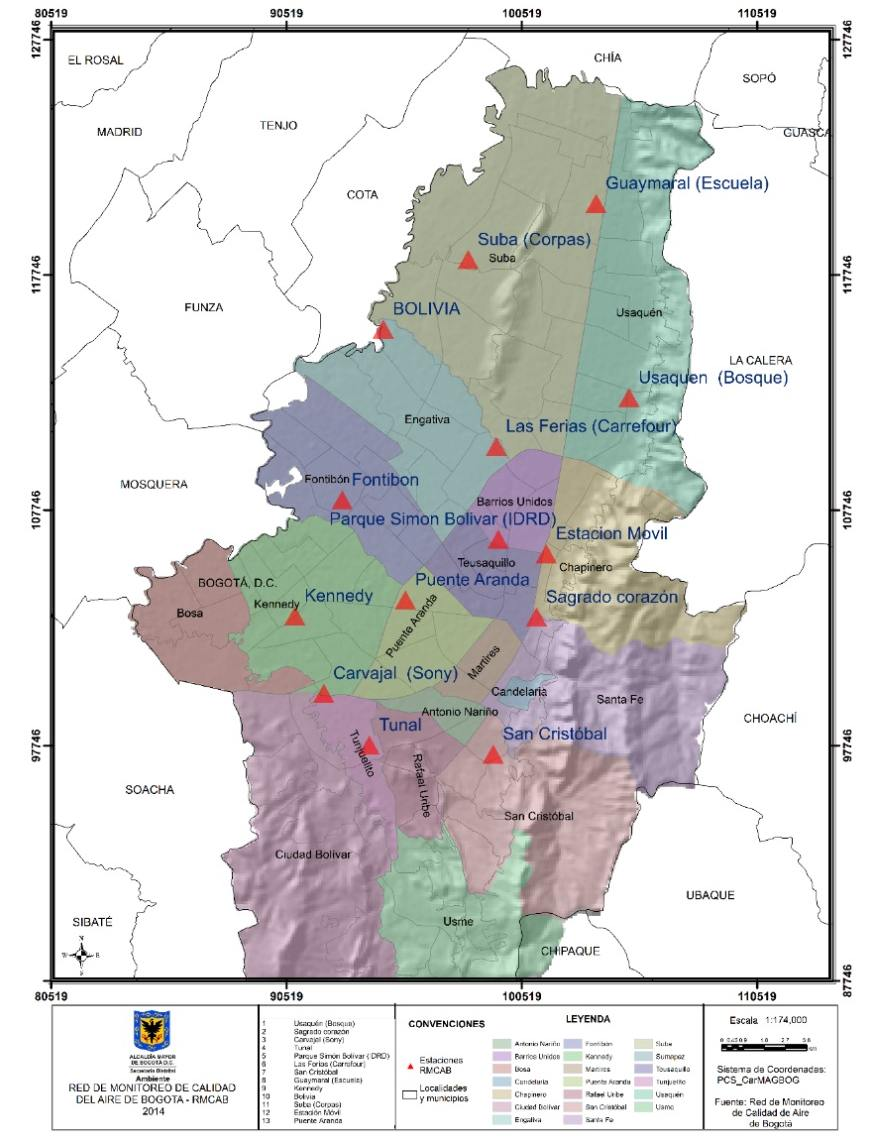
\includegraphics[scale=0.241]{Ubicacion_RMCAB}\end{center}}
& Guaymaral & Fontibón\\\\
& Usaquén & Puente Aranda  \\\\
& Suba & Kennedy \\\\
& Bolivia & Carvajal \\\\
& Las Ferias & Túnal \\\\
& P. Simón Bolívar & San Cristóbal \\\\
& Sagrado corazón & Móvil \\\\
\hline
\hline
\end{tabular}
\\\textbf{Fuente:} http://ambientebogota.gov.co/red-de-calidad-del-aire
\label{tabla:RMCAB}
\end{table}

\begin{table}[!ht]
\begin{center}
\caption{Tabla Clasificación Variables RMCAB.}
\resizebox{16.2cm}{!} {
\begin{tabular}{|l|l|}
\hline
Concentraciones Atmosféricas & Fenómenos  Meteorológicos \\
\hline \hline
Óxidos de Nitrógeno & Precipitación \\ \hline
Dióxido de Azufre & Temperatura \\ \hline
Material Particulados en sus Fracciones Total & Radiación Solar \\ \hline
Material Particulados en sus Fracciones Respirable & Velocidad del Viento \\ \hline
Material Particulados en sus Fracciones Fina & Dirección del Viento \\ \hline
Ozono & Presión Barométrica \\ \hline
Monóxido de Carbono & Húmedad Relativa \\ \hline
Metano &  \\ \hline
Benceno &  \\ \hline
Tolueno &  \\ \hline
Formaldehído &  \\ \hline
Hidrocarburos No Metánicos & \\ \hline
\end{tabular}
}
\label{tabla:variables RMCAB}
\\\textbf{Fuente:} http://ambientebogota.gov.co/red-de-calidad-del-aire
\end{center}
\end{table}


\begin{center}
\chapter{METODOLOGÍA}\label{cap.metodologia}
\end{center}
\section{Resumen}
Para el desarrollo de la investigación y la aplicación de la arquitectura segura computacional, se hizo la consecución de datos de diferentes fuentes de información. Se realizaron las diferentes solicitudes, descargas y archivos de los datos de las tres fuentes: Hospitales Distritales, Secretaría de Medio Ambiente de Bogotá y el Instituto Nacional de Salud. Luego de obtener los datos, se estructuró el desarrollo de la investigación en dos ramas: la minería de datos o explotación de información enfocados hacia la metodología Cross Industry Standard Process for Data Mining (CRISP-DM)  y la seguridad de los datos.

\section{Método Investigativo}
	\subsection{Diseño Metodológico}

Teniendo  en  cuenta el  problema formulado,  el objetivo del proyecto y  el manejo de variables, la  investigación es de carácter experimental, por lo que se manipularán variables independientes, que corresponden a los datos de las fuentes del Hospitales Distritales, Secretaría Distrital de Ambiente de Bogotá y el Instituto Nacional de Salud que darán efecto sobre variables dependientes que corresponde a los resultados dados en el proceso de minería de datos. Las técnicas de minería de datos aplicadas para la investigación son las siguientes:\\\\
\textbf{Método de Clasificación:} el objetivo es predecir la clase a la que pertenecen nuevos objetos a partir de las restantes variables, para determinar que factores de riesgo registrados dentro del Red de monitoreo de calidad de aire de Bogotá (RMCAB) pueden mostrar valores máximos y mínimos en cuanto a problemas críticos ambientales ( temperatura, velocidad del viento, Ozono entre otros), todo esto determinado a través de una legislación ambiental colombiana.\\\\
\textbf{Agrupamiento de datos:} para el caso de los datos obtenidos por parte de los proveedores de  información, los grupos de datos no se encuentran definidos y la forma de aplicar la técnica consiste en obtener grupos naturales a partir de dichos datos, lo que hace que sea necesario definir esos grupos antes de ser analizados. Dentro del método de agrupamiento está la clasificación jerárquica que es aplicada para cada una de los bases de datos ya que no se manejan los mismos atributos dentro de ellas al igual que su contenido y se debe analizar de manera independiente para ser interpretadas.\\\\
El diseño  más  recomendable para abordar este trabajo es el  pre-test, post-test, representado así:\\\\
GOXO\\\\
Donde G corresponde a los datos tomados de cada fuente (entidades involucradas de la investigación), O es la evaluación de los datos seleccionados para la minería de datos o pre-test, X son los procesos perturbación de la información de los Hospitales Distritales para anonimizar los datos, O2 es la técnica de minería de datos a la nueva información después de aplicar la perturbación o post-test, para  contrastarse con O1 y determinar si hay  diferencias significativas en los resultados de los proceso de minería entre antes (datos originales sin perturbación) y después (datos perturbados).
	\subsection{Muestra Poblacional}
    	\subsubsection{Población}
        En la investigación se tuvieron en cuenta tres fuentes de información, que son entidades públicas con los debidos procesos para acceder a los datos:\\

\begin{enumerate}
	\item \textbf{Fuente: Secretaría Distrital de Ambiente de Bogotá:} Es la autoridad ambiental dentro del perímetro del Distrito Capital y entidad rectora de la política ambiental distrital y coordinadora de su ejecución.Está ubicada en la Avenida Caracas No. 54-38 Bogotá. La información requerida será la base de datos de la Red de Monitoreo de Calidad del Aire de Bogotá, en la cual se registran las variables meteorológicas y ambientales respecto a la contaminación de aire. Actualmente se encuentran 13 estaciones de monitoreo, de las cuales doce son fijas y una móvil. La información se solicitó formalmente con los Radicados SDA No. 2016ER142305, 2016ER142728, 2016ER143626 del 18/08/2016 y 2016ER142929, 2016ER142733 del 19/08/2016, de los cuales  se obtuvo respuesta el día 29 de Agosto del año 2016 Ver Anexo A, donde se especifica la información técnica de cada estación y dos direcciones IP para el acceso y descarga de la información que se requiera\footnote{http://201.245.192.252:81} \footnote{http://201.245.192.252:81/App\_Files/Hojas\_de\_Vida\_Estaciones\_2014\%20\%28carpeta\%29.pdf}.
    \item \textbf{Fuente: Hospitales Distritales:}
La información  que se  obtiene para esta investigación es proveniente de fuentes de información externa, recopilada a través de un acceso al servidor del Instituto Nacional de Salud Colombiano, que se ingresa de la siguiente manera:
    \begin{enumerate}
		\item Abrir una hoja de cálculo (excel, openoffice).
        \item Buscar la opción de Fuentes externas, escogiendo el método de conexión Analysis Services, que crea una coexión a un cubo de SQL Server Analysis Service a través de una tabla dinámica.
        \item Ingresar los siguientes datos:
            \begin{itemize}
				\item \textbf{Nombre del Proveedor:} cubos.sispro.gov.co
       			 \item \textbf{Usuario:} sispro.local\textbackslash usuario1
				\item \textbf{Contraseña:} usuario1
	\end{itemize}
    	\item Escoger el tipo de acceso directamente al cubo del SISPRO o de Servicios Públicos.
        \item Para el usuario, escogerá los filtros que utilizará según los datos o columnas que se requieran.
	\end{enumerate}
    
    \item \textbf{Fuente: Instituto Nacional de Salud:} Esta Institución ubicada en la Avenida calle 26 No. 51-20 - Zona 6 CAN. Bogotá, D.C., tiene como fin:
    \begin{enumerate}
		\item \textbf{Investigar:} Para orientar la gestión del conocimiento e innovación en salud y biomedicina de acuerdo con las prioridades y necesidades del país, aportando evidencia científica para la toma de decisiones y la elaboración de políticas en materia de salud pública\footnote{http://www.ins.gov.co/lineas-de-accion/investigacion/Paginas/conoce-la-dreccion.aspx\#.V\_CSQWXxD7Y citada Octubre 01 del 2016 En línea}.  
        \item \textbf{Producir:}  Productos biológicos, biomodelos y reactivos para diagnóstico y referencia que cumplan con los requisitos exigidos, mediante la administración eficaz del sistema de calidad basado en las buenas prácticas de manufactura, buenas prácticas de laboratorio y dentro del marco del Sistema Integrado de Gestión\footnote{http://www.ins.gov.co/lineas-de-accion/Produccion/Paginas/Conoce-la-direccion.aspx\#.V\_CT8GXxD7Y citada Octubre 01 del 2016 En línea}.
        \item \textbf{Vigilar: }  “Vigilan y analizan los posibles riesgos para promover y proteger la salud pública en el territorio Colombiano"   Dr. Mancel Enrique Martínez Durán
Director de Vigilancia y Análisis del Riesgo en Salud Pública.
		\item \textbf{Coordinar:}  “Es un Laboratorio Nacional de Referencia para exámenes de interés en salud pública y se coordinan las redes especiales de Laboratorios, Bancos de Sangre y Trasplantes." Mauricio Beltrán Durán Director Redes en Salud Pública.
        \item \textbf{Observar:}  “El Observatorio Nacional de Salud genera evidencia para apoyar la toma de decisiones en salud del país, liderando la gestión del conocimiento en salud." Carlos Andrés Castañeda Orjuela Director Observatorio Nacional de Salud.
	\end{enumerate}
    La información tiene el mismo origen de los Hospitales Distritales y el mismo método de acceso al anterior.
\end{enumerate}
        
        \subsubsection{Muestra}
        La muestra poblacional corresponde a  los datos nombrados en la investigación, que se seleccionan de las bases de datos de cada fuente la información requerida. De cada fuente se tomará en porcentaje:
        \begin{enumerate}
			\item De los Registros Individuales de Prestación de Servicios de Salud (RIPS) existen 19 columnas, de las cuales una son fechas y las demás son tipo entero, de las que solamente se realizará la aplicación de las técnicas de anonimización a cuatro columnas equivalentes al 20\%. Estas columnas se escogen porque son datos de los rangos de edades vulnerables a sufrir una IRA (0 a 1 años, 1 a 4 años, 70 a 74 años y 75 o más años)
            \item En la Red de Monitoreo de Calidad del Aire de Bogotá (RMCAB) existen aproximadamente 13 tipos de datos, de los cuales se tomará solamente 8 , equivalente al 62\%, siendo los más importantes para el análisis ambiental y que determinan parte importante de las IRA.
            \item Del Sistema Nacional de Vigilancia en Salud Pública SIVIGILA existen 20.000 tipos de datos, de los cuales se tomará solamente 14.000, equivalente al 70\%.
		\end{enumerate}
        
    \subsection{Instrumentos}
    Los instrumentos que se aplicaron a este proyecto de investigación fueron los siguientes:
    \begin{enumerate}
      \item \textbf{Pre-Test:} Esta fase utilizará los datos originales sin procesos, ya que cada proveedor definirá la información para compartir a los demás.
		\item \textbf{RapidMiner:} Es un software para el análisis y la minería de datos. Permite el desarrollo de procesos de análisis de datos mediante el encadenamiento de operadores a través de un entorno gráfico. El fin de este instrumento es poder realizar los dos procesos pre-test y post-test de minería de datos a las fuentes de información seleccionadas.
        \item \textbf{PyCharm CE:} Es un entorno de desarrollo integrado (IDE) usado en la programación en Python. Es desarrollado por la empresa checa JetBrains. Proporciona un análisis de código, un depurador gráfico, un medidor de unidad integrada, integración con sistemas de control de versiones (VCSes) y apoya el desarrollo web con Django, que permitirá el desarrollo de scripts para alterar la información de los RIPS.       
        \item \textbf{Post-Test:} Es la minería de datos perturbados - anonimizados de los RIPS.
        \item \textbf{Análisis del Pre-Test y Post-Test:} Este instrumento permitirá realizar el análisis correspondiente a los tests procesos de minería de datos en el antes y después de la perturbación.
\end{enumerate}
    \subsection{Aplicación de Instrumentos}
La aplicación de los instrumentos se hizo a las fechas establecidas en la Tabla 2.1:
\begin{table}[ht]
\centering
\caption{Cronograma de Aplicación de Instrumentos}
\begin{tabular}{>{\centering\arraybackslash}m{3cm} >{\arraybackslash}m{8cm} }
\hline
\textbf{\textit{Instrumento:}} & \textbf{\textit{Fecha de Inicio - Fecha Final}} \\ \hline
Pre-test & {\centering{Agosto 15 del 2016 - Septiembre 18 del 2016 }} \\ \hline
RapidMiner & {\centering{Septiembre 26 del 2016 - Octubre 10 del 2016 }} \\ \hline
PyCharm CE & {\centering{Septiembre 30 del 2016 - Octubre 10 del 2016 }} \\ \hline
OpenSSL & {\centering{Octubre 11 del 2016 - Octubre 18 del 2016 }} \\ \hline
Post-test & {\centering{Octubre 11 del 2016 - Octubre 14 del 2016 }} \\ \hline
Análisis del Pre-tes \& Post-test & {\centering{Octubre 18 del 2016 - Octubre 26 del 2016 }} \\ \hline
\end{tabular}
\label{tabla:Cronograma}
\\\textbf{Fuente:} Propia.
\end{table}
    \subsection{Análisis de las Fuentes (Primarias, Secundarias, Terciarias)}
    \begin{enumerate}
		\item \textbf{Información Primaria:} Es aquella información que se debe recolectar de las fuentes directas, pero en la investigación no fue requerida.
        \item \textbf{Información Secundaria:} Es aquella que presenta información ya elaborada, o existente. Para la investigación se tomaron los datos de las tres entidades Hospitales Distritales, Secretaría Distrital de Ambiente de Bogotá y el Instituto Nacional de Salud.
	\end{enumerate}
\section{Propuesta de Arquitectura}

La arquitectura computacional segura es la combinación de diferentes técnicas y tecnologías como lógicas y físicas, para salvaguardar la comunicación e intercambio de información entre las entidades. En el caso de la investigación se diseñó a partir de los siguientes elementos (el alcance de la investigación será unicamente a nivel lógico no físico la arquitectura):

\begin{enumerate}
	\item \textbf{Para la Minería de datos:}
    \begin{enumerate}
    	\item \textbf{Objetivo:} Implementar los algoritmos de clasificación y clustering sobre la información de los RIPS, SIVIGILA y RMCAB.
		\item \textbf{Herramienta:} Como herramienta de análisis que permite el desarrollo de procesos de análisis de datos.
        \item \textbf{Técnicas o Métodos:} Aplicar técnicas de clasificación de datos y clustering (agrupación)para el análisis de los datos recibidos por cada ente o proveedor de servicio, con el fín de determinar factores de riesgo que ocasionan enfermedades respiratorias en la ciudad.
    \end{enumerate}
    
    \item \textbf{Para la perturbación:}
    \begin{enumerate}
		\item \textbf{Objetivo:} Lograr perturbar los datos de los RIPS para lograr la anonimización bajo los lineamientos del Ministerio de Salud.
        \item \textbf{Herramienta:} Lenguaje de Programación Python, en PyCharm como Integrated Development Environment (IDE) para desarrollo.
        \item \textbf{Técnicas o Método:} Se aplicará dos técnicas catalogadas como alteración de los datos. La primera se realizará a través de un intercambio de datos mientras que la segunda será una micro-agregación a las columnas seleccionadas.
	\end{enumerate}
    \item \textbf{Para la capa de Transporte/Envió de información:} 
        \begin{enumerate}
		\item \textbf{Objetivo:} Garantizar la comunicación segura a través del protocolo SSL entre los dispositivos.
        \item \textbf{Herramienta:} Librería OpenSSL.
        \item \textbf{Técnicas o Método:} Con la librería nombrada se implementará el protocolo Secure Sockets Layer (SSL) para la comunicación de los dispositivos de la investigación .
	\end{enumerate}
\end{enumerate}
   
\section{Minería de Datos}

\subsection{Modelo de Minería de Datos}

El tratamiento de los datos se hizo a través de un método de minería de datos aplicando agrupamiento (Clustering), en donde se garantiza uniformidad de los datos para ser analizado a traves de la herramienta de analisis. En la agrupación de los datos se cuenta con una serie de elementos de gran importancia, información de datos no agrupados y que buscan tener orden  para determinar su prioridad ya que algunos de los datos no se presentan de manera completa según Fig. 2.1.

\begin{figure}[ht]
\centering
\caption{Fases del modelo de proceso CRISP-DM.} 
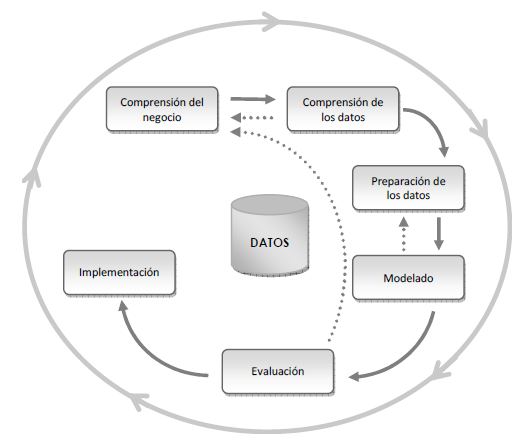
\includegraphics[scale=0.50]{CRIPS}
\\\textbf{Fuente:} http://www.crisp-dm.org/
\label{fig:Ubicacion}
\end{figure}

\begin{enumerate}
	\item \textbf{Preparación de datos:}
    \begin{enumerate}
		
        \item Evaluar los datos recibidos (atributos, datos importantes, datos faltantes).
    	
        \item Verificar que existan los datos suficientes para dicha evaluación c que cubran todas las variables de interés dentro de cada uno de sus atributos.
        
    	\item Evaluar la necesidad de que estos datos sean anonimizados para obtener pruebas y los diferentes resultados finales.
        
	\end{enumerate}
    
    \item \textbf{Selección de datos:}
    \begin{enumerate}
		\item Caracterizar las variables de entrada y de salida para conocer el nivel de importancia dentro de cada una de las bases de datos,tanto los RIPS como SIVIGILA y el RMCAB.
    	\item Identificar el tipo de algoritmo o técnica para realizar de minería de datos.
	\end{enumerate}
    \item \textbf{Mostrar modelo inicial:}
     \begin{enumerate}
		\item Descriptivo para dar a entender el por qué se realizó la minería de datos; de clasificación si se realiza minería para clasificar y finalmente de predicción.
    	\item Dar forma al modelo realizado describiendo  los resultados encontrados sobre la situación actual.
	\end{enumerate}
    \item \textbf{Implementar el modelo:}
      \begin{enumerate}
		\item Revisar los atributos que fueron tomados finalmente para la minería y preparar su respectiva justificación.
    	\item Dar a conocer los resultados finales.
	\end{enumerate}
\end{enumerate}

\section{Perturbación}
Inicialmente en el proceso del cifrado de la información, se aplicará el método de perturbación a los datos tipo médico; el resultado de este método será la anonimización de la información para el momento de querer publicar los datos a entes ajenos al hospital.

Para garantizar la confidencialidad a la información suministrada por las fuentes nombradas anteriormente, se abordó a través del algoritmo AES para el cifrado y descifrado de los datos. Se genera una llave privada de tamaño 128, 192 ó 256 bits. Este método evita que la llave privada se catalogue como débil o semi - débil\footnote{PENCHALAIAH PhD, SESHADRI  PhD. Effective Comparison and Evaluation of DES and Rijndael Algorithm (AES), International Journal on Computer Science and Engineering Vol. 02, No. 05, 2010, 1641-1645 Pág. 1642.} dentro de la clasificación de tipos de claves.
    
    \subsection{Perturbación de Datos}
     Para garantizar la confidencialidad de la información en la base de datos de los Hospitales Distritales, se empleo el método de anonimización a ciertas columnas o datos (carácter médico o personal).\\\\ De esta manera se aplicó la técnica de pertubación (micro agregación de datos) a los datos originales. La perturbación se realizó a partir de la distribución normal o gausiana a datos númericos, que es la distribución de probabilidad normal de variables aleatorias, donde se pueden aproximar a una distribución normal \footnote{ÁNGEL A. Juan, SEDANO Máximo, VILA Alicia. http://www.uoc.edu/in3/emath/docs/Distrib\_Normal.pdf Citado en Septiembre 18 del 2016 Pág. 3. }.

Los pasos en esta fase fueron:
\begin{enumerate}
	\item Selección de los datos a perturbar de las tres bases de datos, justificando su selección y el método a aplicar.
    \item Desarrollo de los Scripts en código Python. Para la investigación se utilizó Sublime Text 2 como editor de código.
    \item Ejecución del script anterior desde consola, utilizando Anaconda\footnote{https://www.continuum.io/downloads} como herramienta para ejecución de archivos de extensión .py.
    \item Verificación de la correcta ejecución del script, tomando las correcciones pertinentes en caso que no sean los resultados esperados.
\end{enumerate}

%	 \subsection{Protocolo SSL}
%     Aprovechando las propiedades del protocolo SSL para el envio y recepción de los datos o archivos entre las partes, se aplicó este protocolo por que garantiza la confidencialidad e integridad de la información. Por su ubicación geográfica diferente y lejana, se utilizó el Internet como medio de comunicación entre los servidores de las tres entidades.\\\\ El protocolo SSL permitirá cifrar la información desde el servidor origen para enviar a los otros dos servidores para su debido descifrado. La información que se envió, implementado el protocolo SSL fue de datos o archivos perturbados y cifrados, generando a través del protocolo la llave privada (para cifrar) y pública (descifrada y enviada por certificación digital).\\\\ Solamente será implementando para realizar la comunicación entre las entidades.\\\\
%Los pasos para la implementación del protocolo SSL, fue dado por:
%\begin{enumerate}
%	\item Búsqueda e instalación de OpenSSL Versión 1.1.0 actualmente estable \footnote{https://www.openssl.org/source/} (herramienta para la implementación del Protocolo SSL) de maneral local.
%    \item Instalación de OpenSSL en otro computador para pruebas de comunicación y envió de la información.
%    \item Ejecución del Protocolo mediante OpenSSL entre los dos computadores.
%    \item Verificación de los resultados esperados tomando las correcciones pertinentes al protocolo.
%\end{enumerate}

     \section{Comparación Datos Cifrados - Originales}
En esta fase se tuvo en cuenta los resultados de los dos procesos de minería de datos aplicados: 
\begin{enumerate}
	\item Minería de Datos a la información original sin perturbación o alteración alguna.
    \item Perturbación - anonimización de los datos sensibles.
%    \item Envío de la información a través del protocolo SSL utilizando OpenSSL.
    \item Minería de Datos a la información perturbada - anonimizada con los mismos pasos del punto N.01.
	\item Comparación y análisis de los dos resultados de minería de datos (Originales - Perturbados).
\end{enumerate}

\begin{center}
 \chapter{MARCO DE REFERENCIA}\label{cap.referencia}
\end{center}

\section{MARCO TEÓRICO}
Las Infecciones Respiratorias Agudas (IRA) constituyen un grupo de enfermedades que se producen en el aparato respiratorio, causadas por diferentes microrganismos como virus y bacterias, que comienzan de forma repentina y duran menos de 2 semanas aproximadamente. Es una de las infecciones más frecuente en el mundo y representa un importante tema de salud pública en nuestro país.  La mayoría de estas infecciones como el resfriado común son leves, pero dependiendo del estado general de la persona pueden complicarse y llegar a amenazar la vida, como en el caso de la neumonía.\\\\
En niños menores de 5 años, la causa de la infección en el  95\% de los casos son los virus, siendo de buen pronóstico; pero un pequeño porcentaje puede padecer complicaciones como  otitis, sinusitis y neumonía. Unos de los efectos que generan gran impacto a nivel local son  la combustión y efectos de cambio climático.\\\\
Se afirma que en países en desarrollo, del 2 al 3\% de los niños presentan enfermedades como neumonía. En invierno es cuando incrementa más la posibilidad de infección viral y también afecta a las mujeres embarazadas y a personas con enfermedades respiratorias.\\\\
Para la investigación, se pretende diseñar una arquitectura que permita compartir información entre diferentes proveedores de información, garantizando la seguridad de los datos confidenciales y poder realizar procesos de análisis de los mismos. De esta manera se escoge la arquitectura multi-partita computacional o Secure Multiparty Computation (SMC) que permite que entidades o datasets tengan sus entradas independientes para alimentar procesos intermedios que generan salidas independiente, cuidando la comunicación segura de las entradas\footnote{DAMGARD Ivan, et at. Multiparty Computation from Somewhat Homomorphic Encryption, International Association for Cryptologic Research 2012, R. Safavi-Naini and R. Canetti (Eds.): CRYPTO 2012, LNCS 7417, pp. 643.} pero ademas, permitiendo compartir trozos o subconjuntos de datos autorizados con otros participantes\footnote{GHODOSI Hossein Ghodosi, et at. Multi-party computation with conversion of secret sharing, Springer Science+Business Media, LLC 2011, Des. Codes Cryptogr. (2012) 62:259–272, Online: 10 May 2011,pp. 260.}. Una expectativa en el proceso SMC es la interacción entre las partes, que permita una funcionalidad independiente pero relacionada para compartir información de manera segura protegiendo la confidencialidad de cada dato\footnote{KIRAZ SABIR Mehmet, UZUNKOL Osmanbey. Efficient and verifiable algorithms for secure outsourcing of cryptographic computations, Springer-Verlag Berlin Heidelberg 2015, Int. J. Inf. Secur, Online: 15 Nov 2015,pp. 1.}.

	\subsection{Minería de Datos}
Un Data Warehouse (DW) o también llamado almacén de datos, es un conjunto de datos orientados a temas integrados, no volátiles e históricos, organizados de tal forma que sirven de apoyo a la toma de decisiones\footnote{INMON, W.H. Building the Data Warehouse 2nd Edition. New York: Wiley, 1996,
401 p. ISBN: 0471-14161-5}, dado que permiten analizar la información consolidada según diferentes puntos de vista. El proceso de consolidación de información involucra actividades
de extracción de diversas fuentes de datos, transformación de la información necesaria y finalmente su carga en el DW. Usualmente se denomina a este proceso ETL, del inglés (Extraction, Transformation and Loading).

Es la Explotación de Información (Data Mining) \footnote{Clark, P.; Boswell R. 2000. Practical Machine
Learning Tools and Techniques with Java
Implementation. Morgan Kaufmann Publisher.}como el proceso mediante el cual se extraen  datos comprensibles y útiles que previamente era desconocidos desde bases de datos, en diversos formatos, en forma automática. Es decir,
la Explotación de Información plantea dos desafíos: por un lado trabajar con gran cantidad de bases de datos y por el otro aplicar técnicas que conviertan en forma automática estos datos en conocimiento.

La aplicación de técnicas de minería de datos permite detectar fácilmente patrones en los datos, razón por la que esta técnica es mucho más eficiente que el análisis dirigido a la verificación cuando se intenta explorar datos procedentes de repositorios de gran tamaño y complejidad elevada. Dichas técnicas emergentes se encuentran en continua evolución, como resultado de la colaboración entre campos de investigación de bases de datos, reconocimiento de patrones, inteligencia artificial, sistemas expertos, estadística, visualización, recuperación de información, y computación de altas prestaciones. Las técnicas de minería de datos se clasifican en dos grandes categorías: supervisados o predictivos y no supervisados o de descubrimiento del conocimiento\footnote{Weiss, S.M. y Indurkhya, N. “Predictive Data Mining. A Practical Guide”Morgan Kaufmann Publishers, San Francisco, 1998.}\\\\
Los algoritmos supervisados o predictivos predicen el valor de un atributo (Etiqueta) de un conjunto de datos, conocidos otros atributos (atributos descriptivos). A partir de datos cuya etiqueta se conoce, se induce una relación entre dicha etiqueta y otra serie de atributos. Esas relaciones sirven para realizar la predicción en datos cuya etiqueta es desconocida. Esta forma de trabajar se conoce como aprendizaje supervisado y se desarrolla en dos fases: Entrenamiento (construcción de un modelo usando un subconjunto de datos con etiqueta conocida) y prueba (prueba del modelo sobre el resto de los datos). Cuando una aplicación no es lo suficientemente madura no tiene el potencial necesario para una solución predictiva, en ese caso hay que recurrir a los métodos no supervisados o de descubrimiento de  conocimiento que descubren patrones y tendencias en los datos actuales (no utilizan datos históricos). El descubrimiento de esa información sirve para llevar a cabo acciones y obtener un beneficio (científico o de negocio) de ellas. En la Figura 3.1 se muestran algunas de las técnicas de minería de ambas categorías.

\begin{figure}[h]
\centering
\caption0{Clasificación de las técnicas de minería de datos} 
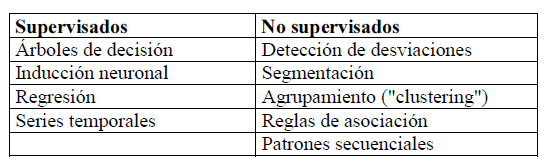
\includegraphics[scale=0.8]{Tabla1}
\label{fig:Tabla1}
\\Fuente Propia
\end{figure}

La aplicación de los algoritmos de minería de datos requiere la realización de una serie de procesos previos con el fin de  preparar los datos de entrada debido a que, en muchas ocasiones los datos proceden de fuentes heterogéneas que no se encuentran organizadas, no tienen el formato adecuado o
contienen ruido. Por otra parte, es necesario interpretar y evaluar los resultados obtenidos. El proceso completo consta de las siguientes etapas\footnote{Cabena, P., Hadjinian, P., Stadler, R., Verhees, J. Y Zanasi, A.
“Discovering Data Mining. From Concept to Implementation”, Prentice Hall, 1998.}:

\begin{enumerate}
\item \textbf{Preparación de Datos:}
	\begin{itemize}
		\item \textbf{Selección:} Identificar las fuentes de información externas e internas y selección del subconjunto de datos necesario.
        \item \textbf{Preprocesamiento:} Estudiar la calidad de los datos y determinar la técnica de minería que se pueden realizar.
\end{itemize}
\item \textbf{Transformación de datos:} Convertir los datos en un modelo para ser analizado.
\item \textbf{Minería de datos:} Realizar tratamiento de los datos seleccionados con una combinación apropiada y de manera funcional.
\item \textbf{Análisis de resultados:} Interpretar los resultados obtenidos en la etapa anterior, generalmente con la ayuda de una técnica de visualización.
\item \textbf{Asimilación de conocimiento:} Aplicación del conocimiento descubierto.
\end{enumerate}

Aunque los pasos anteriores se realizan en el orden en que aparecen, el proceso es altamente iterativo, estableciéndose retroalimentación entre los mismos. Además, no todos los pasos requieren el mismo esfuerzo, generalmente la etapa de pre-procesamiento es la más costosa ya que representa aproximadamente el 60\% del esfuerzo total, mientras que la etapa de minería sólo representa el 10\% . 

\subsection{Clustering}

Como técnica de mineria de datos existe  la de agrupamiento (Clustering) lo que permite clasificar un conjunto de datos. El  K-means es un método particional que intenta encontrar un número específico de grupos, los cuales están representados por sus centroides,aplicable a un grupo de objetos en un espacio continuo n-dimensional. Es uno de los algoritmos de Clustering más antiguos y ampliamente usados.
Es denominado centroide representativo de un cluster el vector formado por las medias de cada una de las componentes de los elementos pertenecientes
al cluster.La técnica general de Clustering K-means es muy simple. A continuación se presenta la descripción del algoritmo básico.\footnote{Tan, Steinbach \& Kumar, 2006.}.

\begin{enumerate}
	\item Seleccionar centroides, donde es el número de clusters deseado.
    \item Asignar cada punto al centroide más cercano,dependiendo del tipo de configuración realizada sobre la herramienta de analisis de datos y cada colección de puntos asignados a un centroide es un cluster.
    \item Actualizar los centroides de cada cluster, basados en los puntos asignados al cluster.Esto dependiendo de que tipo de datos son analizados y que valores son tomados en cuenta.
    
    \item En este caso los valores que se generan en los datos originales son diferentes a los resultados del anonimizado ya que altera valores de manera aleatoria , por lo que la cantidad de valores en cada cluster varia de la misma forma.
   
\end{enumerate}

    \subsection{Criptografía}
    En la actualidad los bancos para los procesos de cifrado y descifrado, están trabajando bajo el estándar de encriptación avanzado AES (Advanced Encriyption Standard), en el cual, la relación entre el consumo computacional y la seguridad que debe garantizar es muy importante, pero en este caso existe un equilibrio para poder trabajar bajo el estándar nombrado. Se deben tener en cuenta los fundamentos generales de la criptografía, donde existe tres campos de acción en el momento de cifrar o proteger cualquier información Cuadro 3.1: 

\begin{table}[ht]
\centering
\caption{Conceptos Generales Cifrados.}\footnote{GOMEZ Vieitis Alvaro. Sistema seguros de acceso y transmisión de datos, RA-MA Editorial Pag 15.}
\begin{tabular}{>{\centering\arraybackslash}m{3cm} >{\arraybackslash}m{9cm} }
\hline
\textbf{\textit{Conceptos:}} & \textbf{\textit{Definición:}} \\ \hline
Criptografía & “...es la ciencia que se encarga de estudiar las distintas técnicas empleadas para transformar (“encriptar” o “cifrar”) la información y hacerla irreconocible a todos aquellos usuarios no autorizados de un sistema informático, de modo que solo los legítimos propietarios puedan recuperar (“desencriptar” o “descifrar”) la información original..." \\ \hline
Criptoanálisis & “...es la ciencia que se ocupa de estudiar herramientas y técnicas que permitan romper los códigos y sistemas de protección definidos por la criptografía..." \\ \hline
Criptología & “...es la ciencia de inventar sistemas de cifrado de la información (criptografía) y de desbaratarlos (criptoanálisis) se la conoce colectivamente con el término de Criptología..." \\ \hline
\end{tabular}
\label{tabla:ConceptosCriptograficos}
\\\textbf{Fuente:} GÓMEZ Vieitis Álvaro. Sistema seguros de acceso y transmisión de datos, RA-MA Editorial.
\end{table}

Además se debe tener en cuenta que los sistemas criptográficos, pueden ser objetos de ataques, para robo o alteración de la información que se esta protegiendo y dando confidencialidad, de esta manera según el criptoanálisis se puede clasificar en 4 tipos:

\begin{enumerate}
	\item \textbf{Ataques basados solo en el texto cifrado:}  “ Se tiene varios textos protegidos con el objetivo de encontrar la clave y recuperar la información original (fuerza bruta)".\footnote{ibi, p. 21}
    \item \textbf{Ataques basados en texto claro conocido:} “ Se tienen varios textos o información cifrados, que se utilizarán para descifrar y encontrar la llave en otros textos.\footnote{ibi, p.  21}
    \item \textbf{Ataques basados en texto claro seleccionado:} “Similar al proceso anterior, pero en este caso se seleccionan los textos cifrados con características similares para descifrar y encontrar la clave en otros textos cifrados".\footnote{ibi, p. 21}
    \item \textbf{Ataques adaptativos basados en texto claro conocido: } “ Con procesos de cifrados anteriores, se busca la estrategia de modificar aquellos procesos por parte, para ir aplicando la modificación sobre los textos cifrados objetos para descifrado".\footnote{ibi, p. 21}
\end{enumerate}

La clasificación de los sistemas criptográficos, dependerá del orígen o naturaleza de las llaves de cifrado / descifrado Figura 3.2, donde existen los procesos simétricos y asimétricos. Los primeros tienen la misma llave para cifrar y descifrar, mientras que en el segundo se generan dos llaves diferentes pero relacionadas entre sí; una para cifrar y otra para descifrar durante el proceso de cifrado. Después de aplicar el sistema de cifrado, la información se debe complementar también de algunas condiciones para garantizar plenamente la confidencialidad y seguridad de los textos u objetos cifrados. Estas condiciones serán dadas por la robustez del esquema de cifrado diseñado y la adecuada gestión de las claves.

\begin{figure}[ht]
\centering
\caption{Clasificación de los sistemas criptográficos.}\footnote{GOMEZ Vieitis Alvaro. Sistema seguros de acceso y transmisión de datos, RA-MA Editorial Pag 23}
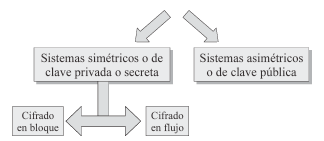
\includegraphics[scale=0.8]{ClasificacionCripto}
\label{fig:ClasificacionCripto}
\\\textbf{Fuente:} GÓMEZ Vieitis Álvaro. Sistema seguros de acceso y transmisión de datos, RA-MA Editorial.
\end{figure}

En el momento de definir la robustez del esquema, se debe definir, a través de métricas, tres propiedades primordiales en el algoritmo aplicado, donde las propiedades son de confusión, difusión y completitud.\footnote{ibi, p. 38} Cuadro. 3.2.\\\\Es realmente difícil poder aplicar un algoritmo con grados altos de las propiedades nombradas, ya que se debe garantizar el buen uso de los servicios y recursos computacionales, trabajando en conjunto con la comunicación para envió y recepción de la información cifrada. Teóricamente el único sistema irrompible es el propuesto por Gilbert Vernam (1917) (Cifrado de Vernam one - time pad) donde con una sola clave que se genera de manera aleatoria y del mismo tamaño del mensaje a cifrar, solamente se dará al impostor la longitud del mensaje, agregando que solo se podrá utilizar una vez dicha clave.

\begin{table}[ht]
\centering
\caption{Propiedades de Robustez en el esquema diseñado de cifrado.}\footnote{GÓMEZ Vieitis Álvaro. Sistema seguros de acceso y transmisión de datos, RA-MA Editorial Pag 38.}
\begin{tabular}{>{\centering\arraybackslash}m{3cm} >{\arraybackslash}m{10cm} }
\hline
\textbf{\textit{Conceptos:}} & \textbf{\textit{Definición:}} \\ \hline
\textbf{\textit{Confusión:}} & “...permite ocultar la relación entre el texto claro y el texto cifrado, dificultando el análisis de patrones estadísticos (se consigue generar la "confusión" mediante operaciones de sustitución de símbolos)..." \\ \hline
\textbf{\textit{Difusión:}} & “...Pretende disimular las redundancias del texto claro al extenderlas por todo el texto cifrado (característica que se consigue gracias a las operaciones de transposición de símbolos)..." \\ \hline
\textbf{\textit{Completitud:}} & “...se cumple si cada bit de texto cifrado depende de todos y cada uno de los bits de la clave. En otro caso, se podrían realizar ataques contra determinadas partes de la clave, en una estrategia de “divide y vencerás”..." \\ \hline
\end{tabular}
\label{tabla:RobustezPropiedades}
\\\textbf{Fuente:} GOMEZ Vieitis Alvaro. Sistema seguros de acceso y transmisión de datos, RA-MA Editorial.
\end{table}

Desde el punto práctico, un sistema criptográfico, se puede medir frente a los ataques de fuerza bruta (se explora todas las posibilidades de claves dentro del rango del sistema criptográfico),  ataques de diccionarios (trabajar con una lista de posibles claves alimentadas de fuentes de información, de la organización dueña de la información) y contra la implementación del algoritmo.\footnote{ibi, p. 39}\\\\
Para la adecuada gestión de claves, se debe definir muy bien los roles de las personas que tengan las claves y los tipos de acceso de la información. La tecnología criptográfica se encuentra sometida a la regulación de la norma International Traffic in Arms Regulations (ITAL)\footnote{ibi, p. 41} porque se cataloga de peligro por el manejo de información cifrada que los gobiernos no puedan descifrar.\\\\
En las características del cifrado AES, para el cifrado avanzado de la información, se compara con otro algoritmo como es DES, el anterior inmediato al AES, donde según el tamaño de claves o llaves, genera un número determinado de llaves:
\begin{itemize}
	\item 128 bits: aproximadamente 3,4 x 1.038 posibles claves\footnote{PENCHALAIAH PhD, SESHADRI  PhD. Effective Comparison and Evaluation of DES and Rijndael Algorithm (AES), International Journal on Computer Science and Engineering Vol. 02, No. 05, 2010, 1641-1645 Pág. 1642.}.
    \item 192 bits: aproximadamente 6.2 x 1.057 posibles claves\footnote{ibi p. 1642.}.
    \item 256 bits: aproximadamente 1,1 x 1077 posibles claves\footnote{ibi p. 1642.}.
\end{itemize}

La investigación implementará el algoritmo AES de longitud 128 bits dentro del protocolo SSL; la comparación con la longitud de DES de 56 bits, donde este se genera 7,2 x 1016 posibles claves, con una diferencia en magnitud de 1021 claves más\footnote{ibi p. 1642.}. Este algoritmo es la última tendencia en el área de seguridad informática en los bancos, entes gubernamentales y de seguridad nacional. Si se quisiera romper la clave generada por el algoritmo DES teóricamente en un segundo, con una máquina de 149 mil millones de dólares, para romper una clave AES, se tardaría 149 billones de años con una longitud de 128 bits\footnote{ibi p. 1642.}. Pero además se tendrá en cuenta las siguientes características:
\begin{itemize}
\item \textbf{Autenticación del funcionamiento del Emisor que envía la información:} La firma digital obtenida a través de la clave privada RSA es imposible de falsificar.\footnote{CELINA Drovandi. CRIPTOGRAFÍA
SEGURIDAD EN ESQUEMAS DE FILE TRANSFER SEGURIDAD EN INTERNET Revista de la Universidad de Mendoza, 2015 pag 374}
\item \textbf{Confidencialidad:} Los datos encriptados no pueden ser interpretados por nadie que no esté autorizado por el Receptor.\footnote{ibid, p. 374.}
\item \textbf{Integridad de la Información:} Cualquier alteración, ya sea accidental o maliciosa de los datos, por mínima que sea, hará que en el proceso de desencriptado la información no resulte clara sino que se transforme en un conjunto ilegible de caracteres.\footnote{ibid, p. 374.}
\item \textbf{Seguridad:} Nadie podrá enviar mensajes falsos intentando usurpar la identidad de un Emisor, ni desde adentro ni desde afuera del sistema.\footnote{ibi, p. 374.}
\item No repudio de origen y destino.\footnote{ibid, p 374.}
\end{itemize}

AES (Advanced Encryption Standard) Se basa en varias sustituciones , permutaciones y transformaciones lineales. Este método es el preferido en procesos de seguridad en los estados, bancos y sistemas de alta seguridad\footnote{Dr. Bhadresh P. Patel, Vishal R. Pancholi. Enhancement of Cloud Computing Security with Secure Data Storage using AES IJIRST –International Journal for Innovative Research in Science and Technology Volume 2 Issue 09 February 2016 ISSN (online): 2349-601 Pag 18}. Una ventaja en el desarrollo del AES permite elegir varios tipos de bits como de 128 bits, 192 bits o clave de 256 bits, por lo que es exponencialmente más fuerte que la clave de 56 bits de DES\footnote{ibi, p. 19}. Además, el proceso de AES comparándolo con DES y RSA, es mejor ya que consumen menos tiempo de cifrado pero mucho mayor de intento de descifrado anormal\footnote{ibi, p. 19}.\\\
El proceso de cifrado AES se compone de una serie de operaciones vinculadas , algunos de los cuales implican la sustituciones específicas y otros implican alrededor de los bits (permutaciones)\footnote{ibi, p.  20}. \\\\ El cifrado AES actualmente se esta implantando e implementando en las tecnologías actuales de la nube, porque es el método más rápido que tiene la flexibilidad y capacidad de ampliación, consumiendo poca memoria a comparación de los otros métodos de cifrado simétrico. En términos de resistencia contra una variedad de ataques tales como ataque cuadrado, clave de ataque, ataque clave de recuperación y el ataque diferencial. Por lo tanto, el algoritmo AES es un método de cifrado de alta seguridad. Los datos también se pueden proteger contra ataques futuros, tales como ataques de la rotura violenta\footnote{ibi, p. 21}. En la actualidad la mayor parte de los algoritmos criptográficos son públicos y se basan en una serie de operaciones elementales sobre los datos que constituyen el texto original: transposiciones (cambiar el orden de los símbolos que forman parte del texto) y sustituciones  (reemplazar unos símbolos por otros)\footnote{GOMEZ Vieitis Alvaro. Sistema seguros de acceso y transmisión de datos, RA-MA Editorial Pag 17}.
    \subsection{Perturbación - Anonimización}
No solamente cifrando la información se podrá dar garantía de confidencialidad de los datos, ya que las personas o entidades que obtengan las claves para descifrar, podrán acceder a la información original. De esta manera, existen varios procesos o técnicas de anonimización de la información, donde es la modificación sistemática de datos, lo que causará que no sean precisas para revelar o identificar registros individuales puntuales \footnote{Dirección de Regulación, Planeación, Estandarización y Normalización DIRPEN. Lineamientos para
la Anonimización de microdatos VERSIÓN: 01 29-08-2014 Pág. 19}.\\\\
Algunos de los métodos de anonimización actuales, se basan en la modificación parcial de los valores de los datos (métodos de perturbación) o cambio de posición de los mismos (métodos de reducción de datos), como se puede observar en los cuadros N. 3.3 y 3.4:\\\\
La perturbación de los datos debe garantizar la privacidad de los datos definidos en las propiedades en el modelamiento de Big Data:
\begin{enumerate}
	\item \textbf{Garantía:} Independiente del proceso o algoritmo de análisis de los datos dentro del Big Data, se debe garantizar que los resultados sean confiables\footnote{SORIA-COMAS Jordi, DOMINGO-FERRER Josep, 
Big Data Privacy: Challenges to Privacy Principles and Models, Data Sci. Eng. (2016) 1(1):21–28,2 Springer, Septiembre 15 del 2015, Pág.23}.
	\item \textbf{Costo Computacional:} Consumo y costo de procesamiento de la información para aplicar el modelo salvaguardando la privacidad\footnote{ibi Pág. 23}.
	\item \textbf{Capacidad de Enlace:} Enlazar varios tipos de dispositivos y fuentes de información\footnote{ibi Pág. 23}.
\end{enumerate}

\begin{table}[ht]
\centering
\caption{Técnicas de Anonimización basados en la perturbación de datos.}
\begin{tabular}{>{\centering\arraybackslash}m{3cm} >{\arraybackslash}m{10cm} }
\hline
\textbf{\textit{Conceptos:}} & \textbf{\textit{Definición:}} \\ \hline
\textbf{\textit{Micro - agregación:}} & “Es reemplazar un valor observado con la media calculada sobre un pequeño grupo de unidades para agregarlos a los datos a perturbar." \\ \hline
\textbf{\textit{Agrupación:}} & “Los registros contenidos en el conjunto original se agrupan en subconjuntos de cardinalidad; por lo menos k mediante algún criterio de similitud."\\ \hline
\textbf{\textit{Sustitución:}} & “Cada registro del conjunto original es sustituido por el registro medio del subconjunto al que ha sido asignado en la etapa anterior." \\ \hline
\textbf{\textit{Intercambio aleatorio de datos - PRAM (Post Randomization Method):}} & “Es un método de control de la difusión estadística que se puede aplicar a los datos categóricos." \\ \hline
\textbf{\textit{Distorsión de datos por una distribución de probabilidades:}} & “Se pretende obtener un conjunto de datos protegido aleatoriamente a partir del conjunto de datos original." \\ \hline
\end{tabular}
\label{tabla:RobustezPropiedades}
\\\textbf{Fuente:} Lineamientos para la anonimización de datos del sistema nacional de estudios y encuestas poblacionales para la salud. Ministerio de Salud Y Protección Social Dirección de Epidemiología y Demografía de Colombia.
\end{table}

\begin{table}[htbp]
\centering
\caption{Técnicas de Anonimización basados en la reducción de datos.}
\begin{tabular}{>{\centering\arraybackslash}m{3cm} >{\arraybackslash}m{10cm} }
\hline
\textbf{\textit{Conceptos:}} & \textbf{\textit{Definición:}} \\ \hline
\textbf{\textit{Eliminación de variables:}} & La primera aplicación de este método es la eliminación de identificadores directos desde el archivo de datos. \\ \hline
\textbf{\textit{Eliminación de registros:}} & Esta técnica consiste en eliminar un registro completo, pero esta altera los resultados estadísticos, por lo que se debe evitar aplicarla.  \\ \hline
\textbf{\textit{Recodificación global:}} & Combina categorías para formar nuevas categorías menos específicas. \\ \hline
\end{tabular}
\label{tabla:RobustezPropiedades}
\\\textbf{Fuente:} Lineamientos para la anonimización de datos del sistema nacional de estudios y encuestas poblacionales para la salud. Ministerio de Salud Y Protección Social Dirección de Epidemiología e Demografía de Colombia.
\end{table}

    \subsection{Protocolo SSL}
Definida la manera de cifrar y anonimizar la información, se debe definir el método o técnica de envió de los datos cifrados y perturbados. El protocolo para aplicar en la investigación será el Secure Sockets Layer (SSL) que provee privacidad y confiabilidad a la comunicación entre dos partes o aplicaciones. El enlace que se genera entre las dos partes es cifrado, que garantizará la privacidad e integridad de los datos\footnote{ SSL Information and FAQ [En línea] <http://info.ssl.com/article.aspx?id=10241> [citado en 18 de Septiembre del 2016]}.\\\\
El protocolo SSL esta diseñado para autenticar el emisor y receptor, así mismo salvaguardar la confidencialidad e integridad de la información. Para el envió de los datos entre las partes, se genera una llave privada para cifrar los datos o archivos, pero es conservada por el emisor. De esta manera, al querer descifrar se aplica una llave pública por el emisor, por medio de un certificado \footnote{Utilizar el protocolo SSL <http://www.4d.com/docs/CMS/CMS02064.HTM> [En línea] [citado en 18 de Septiembre del 2016]} de tipo X.509. El uso de este protocolo es amplio ya que se puede implementar en  navegación web, correo electrónico, fax por Internet, mensajería instantánea, y voz-sobre-IP (VoIP).\\\\
El certificado digital permitirá garantizar la identidad de las partes. El objetivo de este certificado es asociar una clave pública con la identidad del usuario contenida en el certificado\footnote{SEJWANI Sapna, TANWAR Sarvesh, Implementation of X.509 Certificate for Online Applications, International Journal of Research in Advent Technology, Vol.2, No.3, March 2014, E-ISSN: 2321-9637, Pág. 250}, pero se debe tener en cuenta que la seguridad para la autenticación online dependerá de la integridad de la llave pública, ya que si un atacante logra reemplazar la llave pública con la suya, podrá acceder a los datos confidenciales o protegidos\footnote{ibi p. 250.}; pero, este ataque se evita generando una firma digital de una autoridad de certificación, donde la firma es un resumen del mensaje de todos los campos del certificado codificados con la clave privada de la entidad emisora\footnote{ibi p.250.}.\\\\
Para la implementación del protocolo SSL, se utilizará el recurso de OpenSSL \footnote{https://www.openssl.org}, que es un proyecto de caracter de desarrollo libre en C desarrollado por Eric Young y Tim Hudson. Esta herramienta es capaz de operar en sistemas operativos como Linux y
Microsoft Windows; pero también implementando los algoritmos criptográficos: AES, Blowfish, Camellia, SEED, CAST-128, DES, IDEA, RC2, RC4, RC5, TDES, GOST 28147-89, RSA y DSA\footnote{
Velasco Sánchez Paola Maritza, análisis de los mecanismos de encriptación para la seguridad de la información en redes de comunicaciones, facultad de ingeniería maestría en redes de comunicaciones, pontificia universidad católica del ecuador año 2015 Pàg. 28}. Una característica sobresaliente es que permite al sistema implementar el Secure Sockets Layer (SSL), además de ser un robusto paquete de herramientas de administración y bibliotecas relacionadas con la criptografía, que suministran funciones criptográficas a otros paquetes como OpenSSH y navegadores web (para acceso seguro a sitios HTTPS).
    \subsection{Modelo Arquitectónico}
La mayoría de las aplicaciones utilizan la arquitectura vertical, que se cataloga de cliente - servidor, donde las cargas de trabajo se dividen por capas. Pero actualmente se implementa la arquitectura de distribución horizontal, donde cada proceso actuará como cliente y servidor al mismo tiempo\footnote{TANENBAUM Andrew S. VAN Steen Maarte,  “Sistemas Distribuidos, Prinicpios y Paradigmas” Segunda Edición, Pearson Prentice Hall Pág. 44}. Para la investigación se implementará la arquitectura estructurada de punto a punto, que permite que las entidades se comporten como nodos de igual comportamiento. Cada uno será servidor y cliente, según se requiera.
\section{ESTADO DEL ARTE}
	\subsection{Minería de datos }
    
En la actualidad se puede observar grandes cantidades de datos de negocios, sociedades, ciencia, ingeniería, medicina , residen y se procesan en las redes de computadoras o dispositivos de almacenamiento. Este masivo crecimiento es el resultado de los cambios informáticos de la sociedad \footnote{Han, J., M. Kamber, J. Pei. Data Mining -Concepts and Techniques. Morgan Kaufmann,Third Edition (2011).} y como el impulso que dio lugar a la búsqueda de una nueva forma de analizar grandes cantidades de datos, con el fin de obtener información de ellos para la toma de decisiones.\\\\La informatización de las organizaciones tiene como finalidad primera dar soporte a los procesos de negocio básicos. Una vez satisfecho este aspecto, aparece la necesidad de información para buscar nuevas metas de negocio \footnote{Pérez López, C., D. S. Gonzáles. Minería de datos. Técnicas y Herramientas. Ediciones Paraninfo (2007)}.
Esta necesidad es también consecuencia de dos factores importantes, la incertidumbre y el costo por tomar decisiones incorrectas. Esto dio origen al concepto de economía basada en información y conocimiento \footnote{Barreiro Fernández, J., J. Diez de Castro, B.Barreiro Fernández. E. Ruzo Sanmartín, F.Losada Pérez (Coords.). Gestión Científica Empresarial: Temas de Investigación Actuales.Netbiblo (2003)},cuyo objetivo es estudiar las diferentes situaciones que presentan los datos, para adelantarse a ellas y tomar provecho. Uno de los mayores desafíos de las empresas es mantener una cartera de clientes lucrativa. \\\\En este escenario, es necesario adquirir conocimiento que ayude a interpretar las metas, expectativas y deseos de los clientes para poder satisfacerlos de la mejor manera [4].

Es importante resaltar la importancia de utilizar las técnicas de minería  de datos sobre esta serie de investigaciones ya que la cantidad de datos utilizadas en cada una de las bases de datos es muy grande, por mencionar la de los entes públicos y privados.

	\subsection{Privacidad / Anonimización de Datos}
Actualmente la información y los datos de las operaciones de las empresas o entidades, es muy importante para la toma de decisiones; porque la información se convierte en el activo de mayor importancia, ya que a partir de de esta se pueden definir estrategias, decisiones y el paso a paso que se debe realizar en algún momento. Para el caso de la investigación, los datos fueron suministrados de las bases de datos de tres entidades públicas (SIVIGILA, RIPS y RMCAB), en el que los RIPS son las bases de datos que deben garantizar la anonimización y privacidad, por el carácter médico, pues las otras dos bases de datos son de carácter público. Para la investigación se tuvieron en cuenta dos áreas de desarrollo para realizar la propuesta de una arquitectura segura computacional:
    	\subsubsection{Anonimización de Datos}
En el mundo actual, con la tendencia en el avance de la tecnología ha abierto las puertas a nuevas opciones y enfoques para entender y tomar decisiones a partir de enormes cantidades de datos (estructurados, no estructurados y semi estructurados)\footnote{https://www.ibm.com/developerworks/ssa/local/im/que-es-big-data/ Citado el 17 Octubre del 2016 En Línea}, pero también estos grandes volúmenes de datos provienen de diferentes fuentes lo que es un gran desafío para preservar la privacidad y garantía de los datos. Según el objetivo del problema formulado, se tienen  en cuenta variedad de datos como:
\begin{enumerate}
	\item \textbf{Web and Social Media:} esta información es obtenida de las redes sociales (Facebook, Twitter, LinkedIn, blogs entre otros)\footnote{ibi En Línea}.
    \item \textbf{Machine-to-Machine (M2M):} es la información que se obtiene en la conexión de dispositivos de diferentes tecnologías discriminando la transmisión y tipo de datos compartidos\footnote{ibi En Línea}.
    \item \textbf{Big Transaction Data:} disponibles en formatos semiestructurados como no estructurados, que provienen de registros de facturación, telecomunicaciones y registros de llamadas\footnote{ibi En Línea}.
     \item \textbf{Biometrics:} Se incluye huellas digitales, escaneo de la retina, reconocimiento facial, genética entre otros con fines de seguridad\footnote{ibi En Línea}.
     \item \textbf{Human Generated:} Toda la información que una persona del común genera en el diario vivir desde una llamada celular a estudios de créditos\footnote{ibi En Línea}.
\end{enumerate}
Los desafíos actuales del manejo de la información en grandes volúmenes, se enfoca alrededor de las siguientes consideraciones:
\begin{enumerate}
	\item \textbf{Procedencia:} El consentimiento de los proveedores de los datos, independientes si es un individuo o compañía\footnote{SORIA-COMAS Jordi, DOMINGO-FERRER Josep, 
Big Data Privacy: Challenges to Privacy Principles and Models, Data Sci. Eng. (2016) 1(1):21–28,2 Springer, Septiembre 15 del 2015, Pág.22}.
    \item \textbf{Consentimiento:} Sí es simple la autorización, específica, informada y explícitas\footnote{ibi Pág. 22}.
    \item \textbf{Limitación de la finalidad:}Debe ser específica y legítima\footnote{ibi Pág. 22}.
    \item \textbf{Necesidad y minimización de los datos:} Los datos deben ser mantenidos por el tiempo necesario y se deben recoger los datos requeridos\footnote{ibi Pág. 22}.
    \item \textbf{La transparencia y la apertura:} La manera de poder entender los datos y su origen\footnote{ibi Pág. 22}.
    \item \textbf{Derechos individuales:} Derecho a ser olvidado, los proveedores podrán eliminar o rectificar datos sin ninguna restricción\footnote{ibi Pág. 22}.
    \item \textbf{Seguridad de información:}Los datos recogidos deben ser protegidos contra el acceso no autorizado, procesamiento, manipulación errónea, pérdida o destrucción\footnote{ibi Pág. 22}.
\end{enumerate}
En abril del 2016, en la Revista Internacional de Investigación Avanzada en Ingeniería Informática y Comunicación se realizó un consolidado de las propuestas para preservar la privacidad y seguridad de datos en Big Data. La recopilación de las técnicas de punta respecto a la anonimización de datos de manera colaborativa entre diferentes entidades se encuentran:
\begin{itemize}
	\item \textbf{Benjamin C. M. Fung in ”M-Privacy for Collaborative Data Publishing":} Esta propuesta surge de la necesidad de compartir información entre n proveedores, evitando o minimizando el problema de ataques internos de los mismos proveedores. Da solución con el algoritmo de anonimizar el proveedor de datos\footnote{TUPEL Akshaya, PRIYADARSHI Amrit, Data Mining with Big Data and Privacy Preservation, International Journal of Advanced Research in Computer and Communication Engineering IJARCCE ISSN (Online) 2278-1021 ISSN (Print) 2319 5940,
Vol. 5, Issue 4, April 2016, Pág. 1122}. Con el objetivo de publicar una vista anónima de los datos integrados, se quiere proteger contra ataques de agentes externos o internos, que tengan algún conocimiento previo de los datos\footnote{GORYCZKA Slawomir, XIONG Li, FUNG Benjamin C. M, m-Privacy for Collaborative Data Publishing, IEEE TRANSACTIONS ON KNOWLEDGE AND DATA ENGINEERING, VOL. 26, NO. 10, OCTOBER 2014, pÁG. 2521.}. 
    \item \textbf{Madhuri Patil in ”Privacy Control Methods for Anonymous And Confidential Database Using Advance Encryption Standard”:} Implementando la tecnología de encriptación AES, se utiliza el protocolo criptográfico Diffie-Hellman, para establecer la comunicación entre partes o proveedores que no han tenido contacto previo, utilizando un canal inseguro, y de manera anónima (no autentificada)\footnote{TUPEL. Op. cit., 1122.} para compartir las claves aunque sea en una red pública. La privacidad de la información se puede dar con un enfoque criptográfica, aprendizaje de máquina, aleatorización, y K-clustering\footnote{PATIL Madhuri, Ingale Sandip, Privacy Control Methods for Anonymous \& Confidential Database Using Advance Encryption Standard, IJCSMC, Vol. 2, Issue. 8, August 2013, pg.224 – 229, Pág. 225.}.
    \item \textbf{Noman Mohammed and Benjamin C. M. FUNG in ”Centralized and Distributed Anonymization for High Dimensional Healthcare Data Description”:} El autor considera que centralizar y anonimizar los datos distribuidos es importante para preservar la seguridad y privacidad, implementando el modelo LKC para aplicarlo en un entorno centralizado y distribuido\footnote{TUPEL. Op. cit., 1122.}
\end{itemize}
\subsection{Aplicaciones Recientes}
Con arquitecturas de  este  tipo se ha incursionado  en  algunos gremios,en algunas oportunidades con casos fallidos  y en otras con casos exitosos. Como caso fallido se tiene  la eventualidad en la  ciudad de New York en el año 2014, cuando se recopiló la información de todos los taxistas de la ciudad por parte de la alcaldía neoyorkina. Pero una falla en el proceso de cifrado MD5 permitió que personas ajenas recuperaran información personal de los taxistas de alrededor de 173 millones de viajes realizados\footnote{DAN Goodin.Poorly anonymized logs reveal NYC cab drivers’ detailed whereabouts [En linea]. New York: Dirección URL: <http://arstechnica.com/tech-policy/2014/06/poorly-anonymized-logs-reveal-nyc-cab-drivers-detailed-whereabouts/>. [30, Marzo 2015].}, dejando en evidencia sus datos personales y las rutas con sus clientes frecuentes,  perjudicando así su privacidad. Si esta información la obtuvieran grupos criminales podrían dar seguimiento a taxistas y pasajeros.\\\\
Un caso exitoso fue el de Netflix, cuando en el año 2006 logró anonimizar la información de más de 500.000 millones de clientes junto a las preferencias de los mismos, mostrando un grado de nivel alto de seguridad y preservación de la integridad de los datos\footnote{HERNANDEZ Alexander New York taxi details can be extracted from anonymised data, researchers say [En linea]. New York: Dirección URL: <https://www.theguardian.com/technology/2014/jun/27/new-york-taxi-details-anonymised-data-researchers-warn>. [30, Marzo 2015].}.\\\\

\section{MARCO LEGAL}
\subsection{Legislación Nacional}
En Colombia la legislación vigente referente a la protección de la confidencialidad se encuentra consagrada en la Constitución Política, en el Artículo 15:\\
"Todas las personas tienen derecho a su intimidad personal y familiar y a su buen nombre, y el Estado debe respetarlos y hacerlos respetar. De igual modo, tienen derecho a conocer, actualizar y rectificar las informaciones que se hayan recogido sobre ellas en los bancos de datos y en archivos de entidades públicas y privadas. En la recolección, tratamiento y circulación de datos se respetarán la libertad y demás garantías consagradas en la Constitución. La correspondencia y demás formas de comunicación privada son inviolables"\footnote{De Colombia CP Constitución Política de Colombia Bogotá Colombia Leyer 1991}.\\\\
En 2012, la Ley 1581, por la que se dictan disposiciones generales para la protección de datos personales, parcialmente reglamentada por la Ley 1377 de 2013, dispone en sus principios referentes al acceso y circulación restringida de seguridad y de confidencialidad, que el acceso a los datos se debe restringir y la información debe estar sujeta a tratamiento por parte del responsable, como lo indica en el Artículo 4. Finalmente, en el Código Nacional de Buenas Prácticas para las Estadísticas Oficiales se hace referencia a la anonimización de los micro-datos en el principio 5:\\\\
Confidencialidad. Las entidades pertenecientes al Sistema Estadístico Nacional -SEN- deben garantizar la protección y la confidencialidad de la información con la que se producen las estadísticas oficiales, así como evitar la identificación de las fuentes.\footnote{CUARTAS Rodriguez E, JALLER Escudero JD. El Habeas Data como Derecho fundamental y la Ley 1581 de 2012 y su decreto 1377 de 2013-2014}. El numeral 5.3  precisa que se debe:
"Asegurar que la publicación de las estadísticas oficiales no permita la identificación individual de las fuentes"\footnote{ibi p. 3}.
Adicionalmente en los numerales 5.4 y 5.6 el Código enfatiza que se debe contar con un protocolo para anonimizar los datos.
"5.4 Aplicar protocolos para la protección y seguridad de la información". "5.6. El acceso a micro-datos anonimizados por parte de los usuarios debe estar sujeto a protocolos que garanticen la confidencialidad"\footnote{ibi p. 3}.\\\\
La Ley 1581 de 2012 en su Artículo 21, da las pautas para la divulgación total o parcial, indicando que la información puede tener una versión pública siempre y cuando mantenga la reserva únicamente de la parte indispensable:
Principio de la divulgación proactiva de la información. El derecho de acceso a la información no radica únicamente en la obligación de dar respuesta a las peticiones de la sociedad, sino también en el deber de los sujetos obligados de promover y generar una cultura de transparencia, lo que conlleva la obligación de publicar y divulgar documentos y archivos que plasman la actividad estatal y de interés público, de forma rutinaria y proactiva, actualizada, accesible y comprensible, atendiendo a límites razonables del talento humano y recursos físicos y financieros\footnote{Congreso de la República Ley 1712 de 2014.}.
\subsection{Legislación Ambiental Nacional}
El Ministerio de Ambiente, Vivienda y Desarrollo Territorial establece con la Resolución 601 de 2006, la Norma de Calidad del Aire o Nivel de Inmisión, donde se especifica los contaminantes y sus niveles de tolerancia, así mismo las entidades responsables de control y seguimiento en el territorio colombiano. Para la investigación será importante tener como referencia las Figuras 3.3, 3.4 y 3.5 para compararlas con los resultados de la minería de datos.
\begin{figure}[h]
\centering
\caption{Niveles máximos permisibles para contaminantes criterio.} 
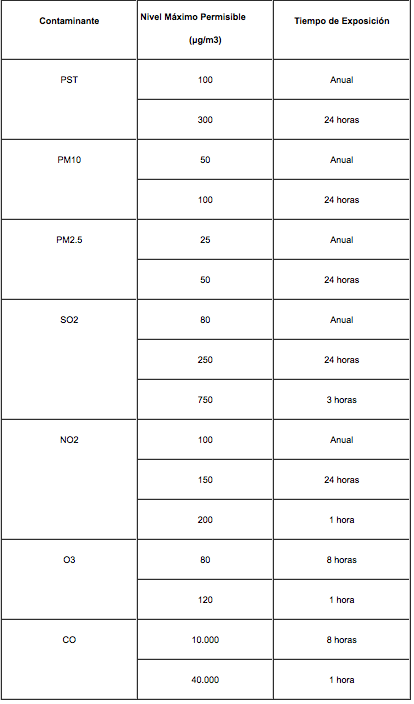
\includegraphics[scale=0.57]{Norma1}
\\\textbf{Fuente:} http://www.alcaldiabogota.gov.co/sisjur/normas/Norma1.jsp?i=39330
\label{fig:Ubicacion}
\end{figure}

\begin{figure}[h]
\centering
\caption{Niveles máximos permisibles para contaminantes no convencionales con efectos carcinogénicos.} 
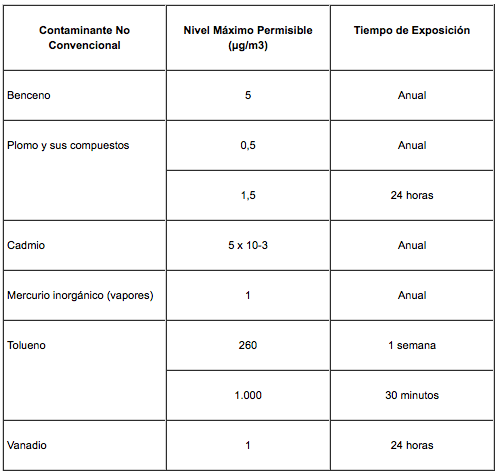
\includegraphics[scale=0.56]{Norma2}
\\\textbf{Fuente:} http://www.alcaldiabogota.gov.co/sisjur/normas/Norma1.jsp?i=39330
\label{fig:Ubicacion}
\end{figure}

\begin{figure}[htp]
\centering
\caption{Concentración y tiempo de exposición de los contaminantes para los niveles de prevención, alerta y emergencia.} 
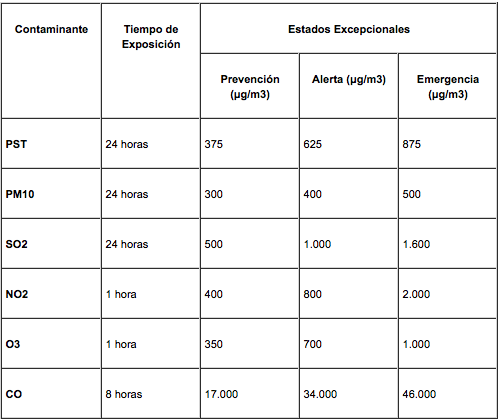
\includegraphics[scale=0.56]{Norma4}
\\\textbf{Fuente:} http://www.alcaldiabogota.gov.co/sisjur/normas/Norma1.jsp?i=39330
\label{fig:Ubicacion}
\end{figure}


\subsection{Legislación Internacional}

Según el principio establecido por la División de Estadísticas de Naciones Unidas, los datos deben ser manejados con confidencialidad y exclusividad.
Los datos que reúnan los organismos de estadística para la compilación estadística, ya sea que se refieran a personas naturales o jurídicas, deben ser estrictamente confidenciales y utilizarse exclusivamente para fines estadísticos\footnote{ONU United Nations Statistical Commission. Fundamental principles of official statistics. Off Rec Econ Soc Counc. 1994.}.

En el contexto jurídico, la Unión Europea, desde su Directiva 95/46/CE, en el considerando 26, excluye los datos anonimizados del alcance de la legislación sobre protección de los mismos considerando que:

"Los principios de la protección deberán aplicarse a cualquier información relativa a una persona identificada o identificable"; que, para determinar si una persona es identificable, hay que considerar el conjunto de los medios que puedan ser razonablemente utilizados por el responsable del tratamiento o por cualquier otra persona, para identificar a dicha persona; que los principios de la protección no se aplicarán a aquellos datos hechos anónimos de manera tal que ya no sea posible identificar al interesado; que los códigos de conducta con arreglo al artículo 27 pueden constituir un elemento útil para proporcionar indicaciones sobre los medios, gracias a los cuales los datos pueden hacerse anónimos y conservarse de forma tal que impida identificar al interesado\footnote{Unión Europea UE. Europeas C, de la Unión Europea C. Directiva 95/46/CE del Parlamento Europeo y del Consejo de 24 de octubre de 1995 relativa a la protección de las personas físicas en lo que respecta al tratamiento de datos personales ya la libre circulación de estos datos. Agencia de Protección de Datos; 1997.}.

\begin{center}
 \chapter{DESARROLLO DEL PROYECTO}\label{cap.desarrollo}
\end{center}
\section{Recolección de la información}
\subsection{Hospitales Distritales}
Los datos recibidos por parte del Registro Individual de Prestación de Servicios de Salud (RIPS), cargados a la bodega de datos, corresponden a los datos de los archivos de usuarios, consultas, procedimientos, urgencias y hospitalizaciones; Figura 4.1. Con estos reportes, los usuarios podrán consultar y analizar las atenciones de salud a nivel nacional y territorial, navegando a través de las dimensiones y medidas disponibles; esto dependiendo de la necesidad y la manera en que se interpretarán los datos.

\begin{figure}[ht]
\centering
\caption{Datos RIPS} 
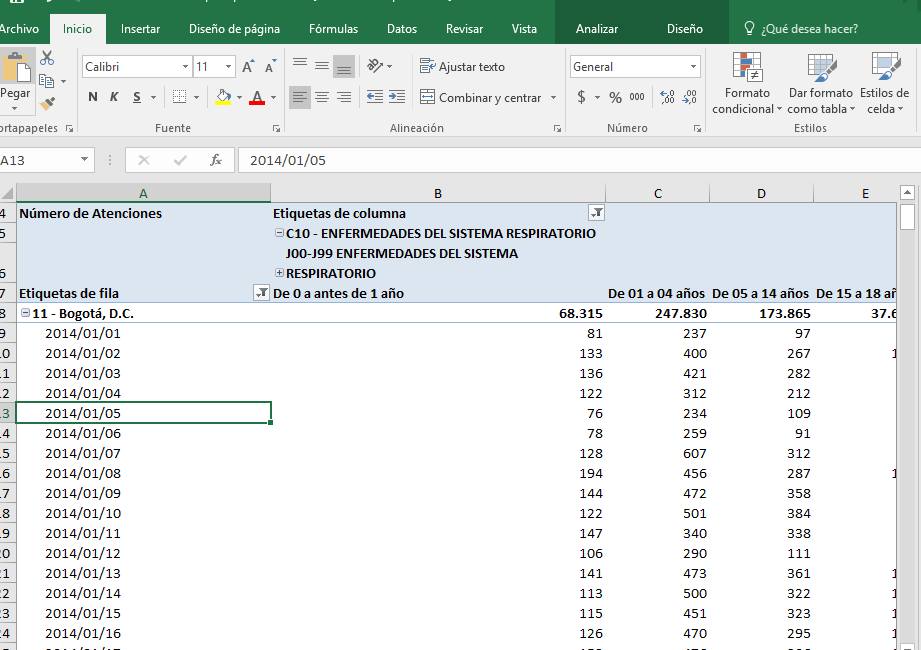
\includegraphics[scale=0.6]{prepa2}
\label{fig:Rips6}
\\ \textbf{Fuente:} Propia.
\end{figure}

Para tener acceso a la información generada por parte de los hospitales distritales es necesario acceder  a la base de datos principal por medio de la herramienta de  hoja de cálculo para tener una base de la información para este caso (CUBO), que es procesamiento Analítico en Línea y que se encuentra constantemente conectado en la red. Contiene datos a nivel general de todos los centros hospitalarios y es allí donde se puede consultar reportes predefinidos o elaborar propios reportes según las necesidad de información. A través del sistema de gestión de datos SGD, por ejemplo, un mismo dato “número de afiliados a salud” puede ser analizado bajo distintos puntos de vista: componente de la protección social, fecha de afiliación, sexo, administradora y/o departamento. El análisis de datos a través de diversas dimensiones permite detectar comportamientos y reglas del negocio que no son fácilmente identificables con los sistemas transaccionales,
donde se encuentra recolectada la información con la que realizará el análisis inicial.

\subsection{Instituto Nacional de Salud}

1. Al igual que en la anterior información el instituto nacional de salud tiene conexión a través del cubo. A través de la fuente de información se selecciona la Opción de Sivigila para tener acceso a la información por parte del Instituto Nacional de salud. Figura 4.2.

\begin{figure}[ht]
\centering
\caption{Acceso a SIVIGILA} 
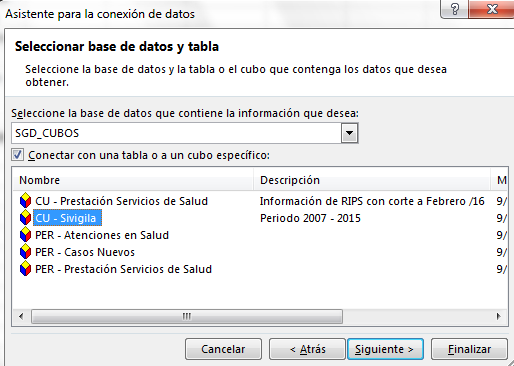
\includegraphics[scale=0.6]{Rips5}
\label{fig:Rips6}
\\ \textbf{Fuente:} Propia.
\end{figure}

\subsection{Secretaría Distrital de Medio Ambiente}
1. Para realizar la recolección de los datos de la Red de Monitoreo de Calidad del Aire de Bogotá (RMCAB), se procede de manera directa a la dirección : http://201.245.192.252:81/ en los link  “Publicaciones/Informes Anuales” y “Publicaciones/Informes Trimestrales y Semestrales” y en la página del Observatorio Ambiental de Bogotá,  en el link de aire. - See more at: 
http://ambientebogota.gov.co/red-de-calidad-del-aire\#sthash.kwnJsI4H.dpuf.

2. Para el caso de las estaciones de monitoreo en la parte  izquierda dentro de la página aparecerá el listado de reportes que puede tener interacción de manera permanente. Los reportes que se quieren generar son específicos y dependen de lo que se quiera revisar, en este caso las fechas, la estación , la periodicidad del monitoreo.Esta serie de elementos forman parte del resultado que arroje el reporte y que valor se le da a la hora de ser analizado.

\begin{figure}[ht]
\centering
\caption{Datos de RMCAB} 
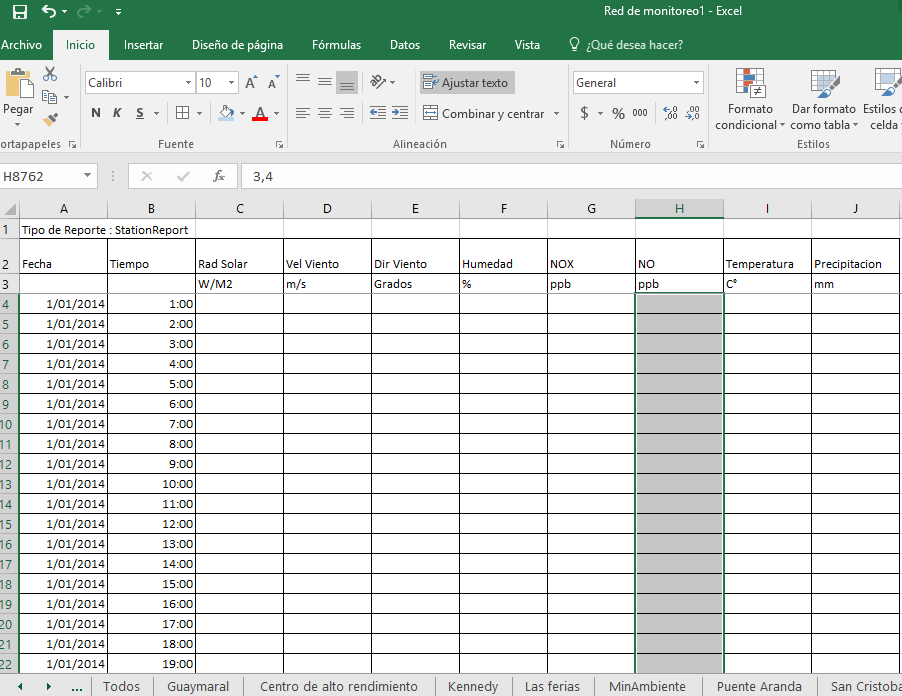
\includegraphics[scale=0.6]{SeleccionDato}
\label{fig:Rips6}
\\ \textbf{Fuente:} Propia.
\end{figure}

\section{Minería de Datos}

\begin{enumerate}
	\item \textbf{Preparación de datos:}
    \begin{enumerate}
		\item Evaluación de los datos: para realizar la evaluación de los datos suministrados por parte de los proveedores de datos, se  dio a la tarea de revisar cada una de las bases de datos para interpretarse de manera lógica y entendiendo la referencia que este presenta para cada uno de los entes,  de manera tal, que  estos datos tuvieran un orden para entenderse al ser utilizados.

\begin{figure}[ht]
\centering
\caption{Evaluación y alistamiento de datos} 
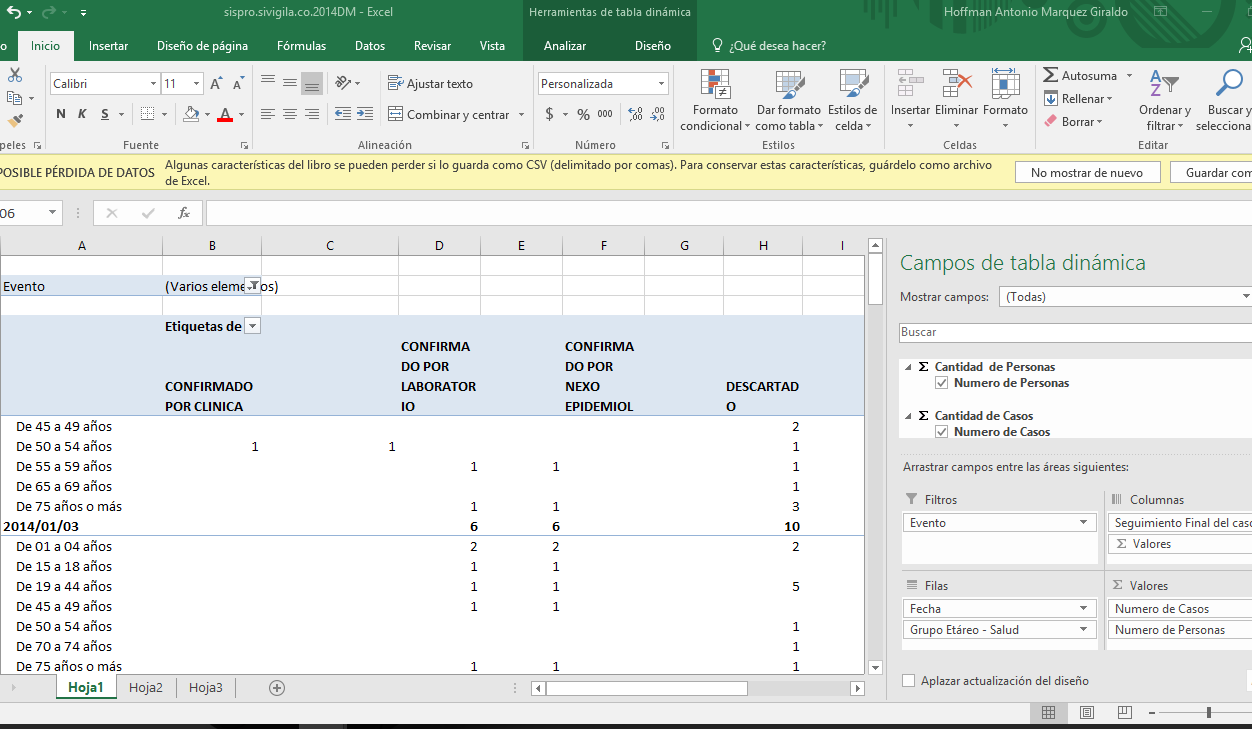
\includegraphics[scale=0.3]{DatoCsv}
\label{fig:1_OpenSSL}
\\ \textbf{Fuente:} Propia.
\end{figure}

    	\item Verificación de los datos: para los datos que suministra el cubo, permite consultar y elaborar reportes a partir de una construcción dinámica que se obtiene con la navegación de los elementos fundamentales de una bodega de datos: dimensiones y medidas , también las fechas .
	\end{enumerate}
    \item \textbf{Selección de datos:}
    \begin{enumerate}
		\item Caracterización de  las variables de cada una de las bases de datos,de los RIPS, SIVIGILA y el RMCAB. Los datos que se seleccionaron para realizar el análisis tuvieron que ser filtrados por sus atributos. Esto dependía de la información  de cada una de las fuentes, debido a que estas no manejan una información homogénea y requería elegir datos que a la hora de realizar una técnica de minería de datos no arrojara valores en blanco. Figura 4.4 y 4.5.


\begin{figure}[h]
\centering
\caption{Evaluación y preparación de datos} 
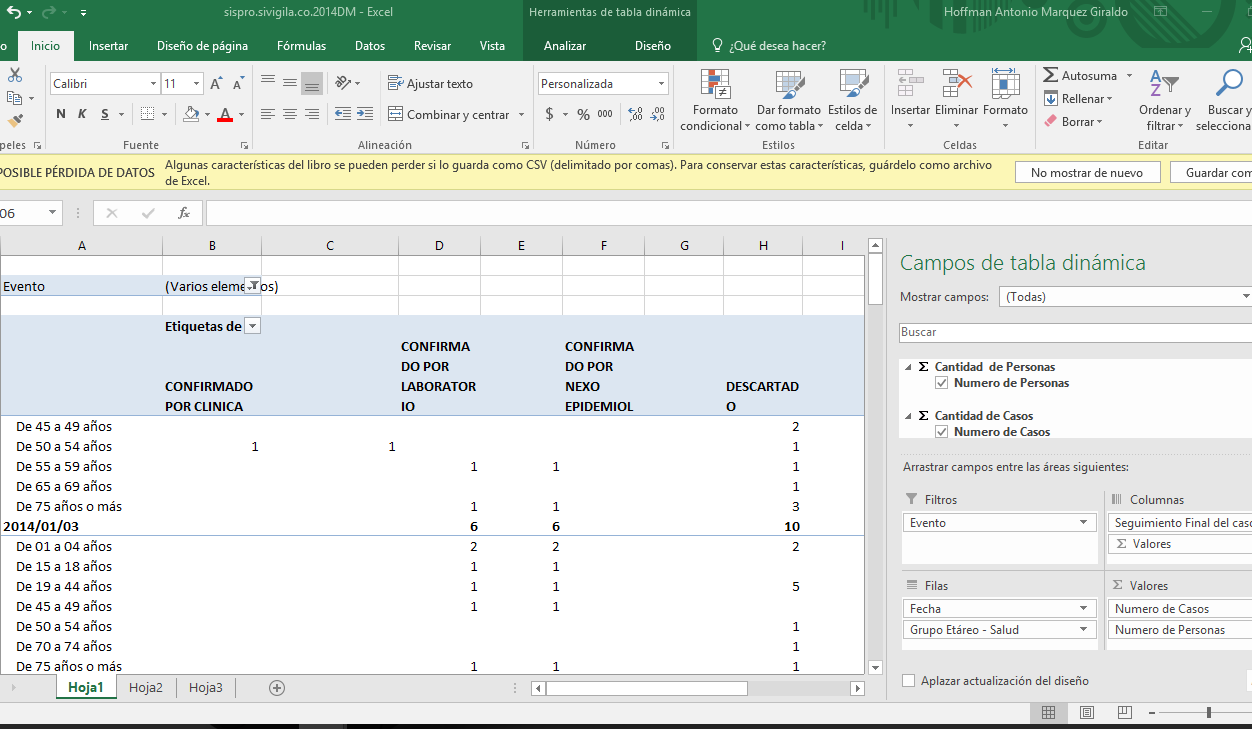
\includegraphics[scale=0.3]{DatoCsv}
\label{fig:1_OpenSSL}
\\ \textbf{Fuente:} Propia.
\end{figure}

    	\item Identificación del tipo de algoritmo o técnica a realizar de minería de datos para cada base de datos.
	\end{enumerate}
    \item \textbf{Modelo Inicial de Minería de Datos}
     \begin{enumerate}
		\item Inicialmente se determinó que para realizar un análisis de cada una de las bases de datos, se debe tener en cuenta los atributos con los que se esta trabajando en estos momentos y todos los relacionados con el tema ambiental y de carácter epidemiológico que abarcan las enfermedades del sistema respiratorio en relación con la IRA.
	\end{enumerate}
    \item \textbf{Implementación del modelo:}
      \begin{enumerate}
		\item Aplicar el modelo definidos para la minería de datos a la información original:


Al aplicar la agrupación de los datos con relación a cada una de las bases de datos, los análisis generados en la herramienta de RapidMiner muestran la variación que se produce en tiempos donde más se emiten contaminantes. En la tabla 4.6 se puede observar: 

\begin{figure}[ht]
\centering
\caption{Datos generales  RMCAB} 
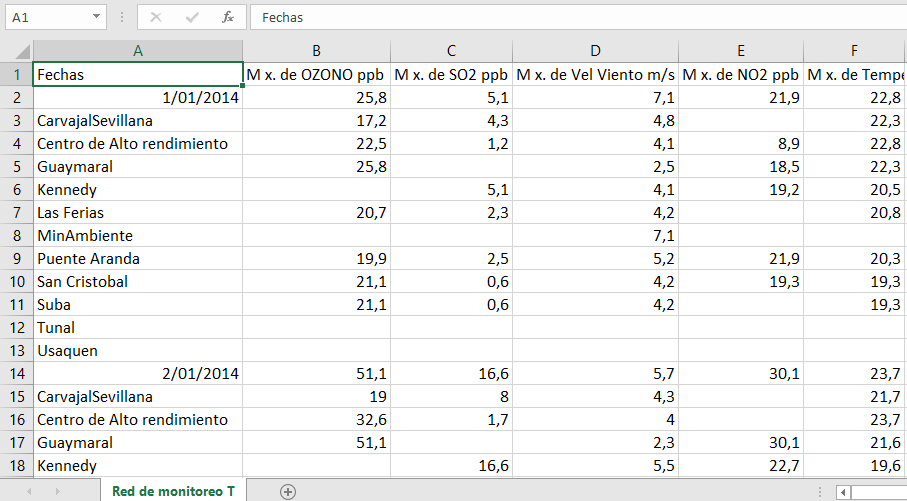
\includegraphics[scale=0.4]{VgRMCAB}
\label{fig:1_OpenSSL}
\\ \textbf{Fuente:} Propia.
\end{figure}        
 
         \end{enumerate}
          \end{enumerate}

\section{Perturbación}
Para los datos de tipo entero o numéricos se aplicó la distribución Gaussiana o Normal, para la alteración de los valores y para las cadenas el intercambio de posición; de esta manera se garantizará la anonimización de los datos.
    
    \subsection{Perturbación de Datos}

\begin{enumerate}
	\item \textbf{Selección de los datos a perturbar:} Se aplicaron dos técnicas diferentes sobre las mismas columnas bajo los lineamientos del Ministerio de Salud y Protección Social de Colombia y el DANE, para publicar datos de información de enfermedades epidemiológicas del territorio nacional. Las variables de la bases datos de los RIPS, son de tipo numérico, excepto la fecha donde será alfanumérico. Según los lineamientos tratados, las técnicas pertinentes para aplicar en las variables o datos numéricos encontradas en archivo de extensión .xls fueron:
    \begin{itemize}
    	\item Micro agregación, donde se debe encontrar la media del conjunto a perturbar, en el momento de calcular la media aritmética se sumará al dato que se anonimizará.
        \item Permutación, se aplica al intercambiar las posiciones entre los datos salvaguardando las características estadísticas como el promedio, la variación estándar, desviación entre otras.
    \end{itemize}
La figura 4.8 , refleja la estructura del archivo a leer y perturbar, así mismo, se evidencia el tipo de variable de las diferentes columnas.
  \begin{figure}[!ht]
\centering
\caption{Estructura de los Datos RIPS} 
 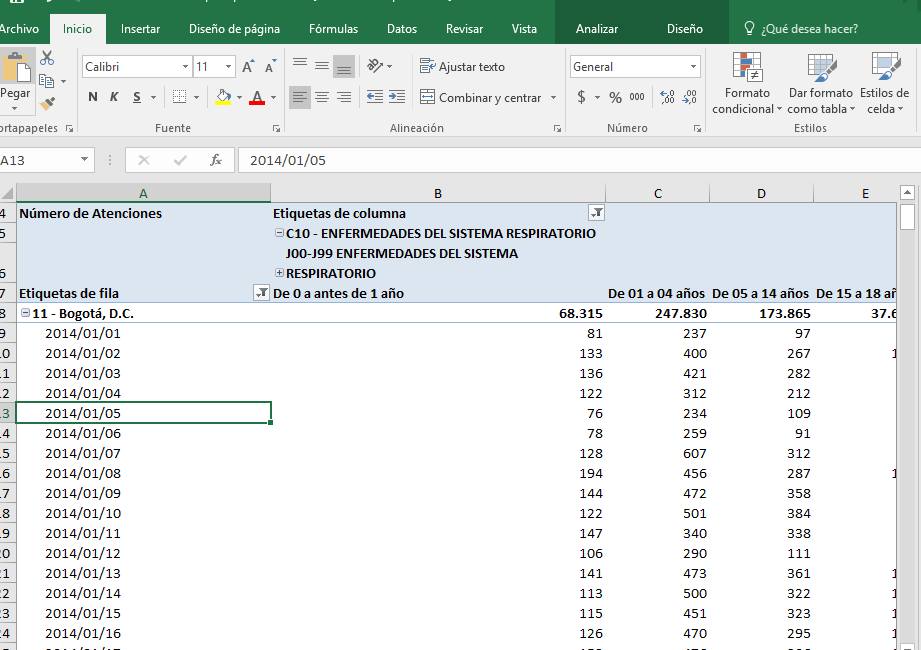
\includegraphics[scale=0.46]{Datos_Rips}
\label{fig:Datos_Rips}
\\ \textbf{Fuente:} Propia.
\end{figure}    
    \item \textbf{Desarrollo del Script para Anonimizar los datos RIPS en Python. Ver anexo B.}
   \item \textbf{Ejecución del Script:}  Para la ejecución dentro de la investigación y experimento, se ejecutó el código desde consola o línea de Comandos y en el ambiente de Anaconda (Python). Como se ve reflejado en la figura 4.9.\\\\El código se encuentra en el anexo B desarrollado desde la línea \textbf{1} a la línea \textbf{11}, solamente se importa las librerías necesarias junto con los arreglos y variables necesarias (La línea \textbf{11} determina las cuatro columnas en que se aplicará la anonimización). Desde la línea \textbf{12} a la línea \textbf{12} hará la lectura del archivo donde se encuentran los datos para recuperarlos y guardarlos en las listas declaradas dentro una lista, junto con el cálculo de los datos a perturbar. Ahora desde la línea \textbf{16} a la línea \textbf{28} se realiza el proceso de filtro y limpieza de los datos repetidos, vacíos o que no son útiles para la investigación.\\\\
Para la línea \textbf{29} a la línea \textbf{32}, se aplica el proceso de permutación de los valores utilizando shuffle de la librería Numpy, para organizar las listas de las columnas de manera aleatoria, ya que desde la línea \textbf{33} se realiza la escritura de todas las columnas recuperadas anteriormente en un archivo de extensión .csv para ser leído posteriormente por RapidMiner.\\\\Para el proceso de perturbación por Micro agregación, se declara como k=3 donde se verá reflejado en la línea \textbf{41} (Número de variables por sub grupo); desde la línea \textbf{43} a la línea \textbf{72}, se realiza el proceso de anonimización de datos por microagregación. Finalmente desde la línea \textbf{83} se realiza la escritura con los datos anonimizados.
\begin{figure}[ht]
\centering
\caption{Ejecución del Script desde consola o Línea de Comandos, con run y la ruta junto con el nombre del Script.} 
 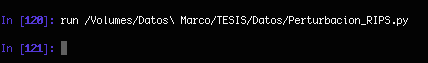
\includegraphics[scale=0.85]{Ejecucion_Python}
\label{fig:Ejecucion_Python}
\\ \textbf{Fuente:} Propia.
\end{figure}
    \item \textbf{Resultado de la Ejecución del Script de Perturbación - Anonimización:} El script se desarrolló con el objetivo de aplicar tres técnicas diferentes de anonimización en seis columnas de manera aleatoria, los datos serán diferentes cada vez que se ejecute el script, garantizando anonimización de los mismos. 
\end{enumerate}
%	 \subsection{Protocolo SSL}
%\begin{enumerate}
%	\item \textbf{Búsqueda e instalación de OpenSSL\footnote{https://www.openssl.org/source/} de manera local según cuadro 4.1:}
%\begin{table}[h]
%\centering
%\caption{Paso a paso Instalación de OpenSSL}
%\begin{tabular}{>{\centering\arraybackslash}m{11cm} >{\arraybackslash}m{4cm} }
%\hline
%\textbf{\textit{Paso a paso}} & \textbf{\textit{Alcance o Actividad}} \\ \hline
%{\begin{center}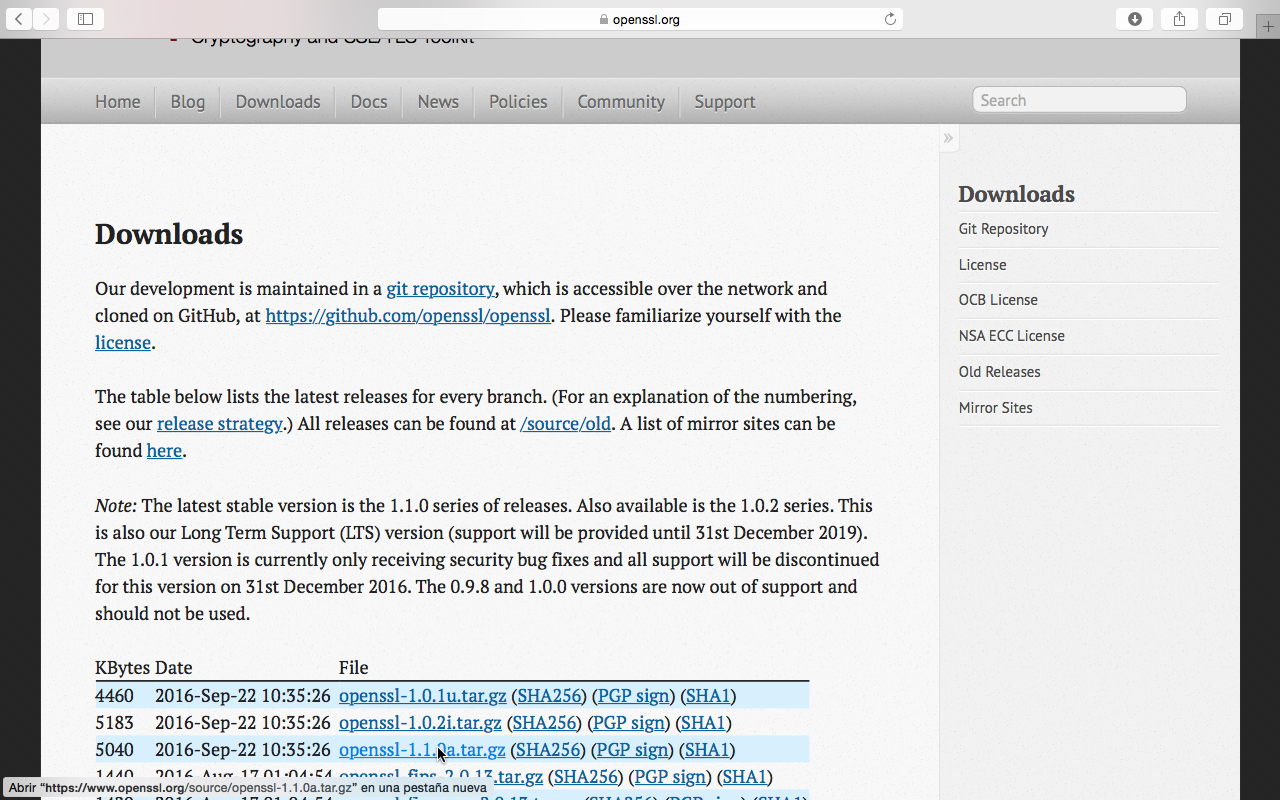
\includegraphics[scale=0.2]{openssl/1_OpenSSL}.\end{center}} & En el buscador de Internet se ingresa al siguiente link \footnote{https://www.openssl.org/source/}, en el cual se buscará la versión 1.1.0 que actualmente es la más estable según la documentación de la herramienta. \\ \hline
%{\begin{center}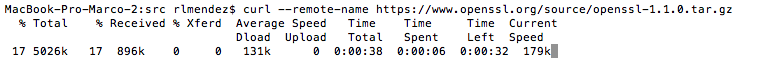
\includegraphics[scale=0.42]{openssl/2_OpenSSL}.\end{center}} & Se abre un terminal en el equipo, para descargar el paquete. \\ \hline
%{\begin{center}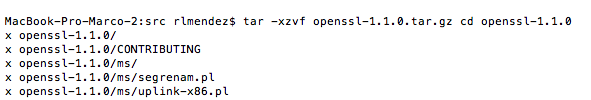
\includegraphics[scale=0.5]{openssl/3_OpenSSL}.\end{center}} & Extraer el archivo. \\ \hline
%{\begin{center}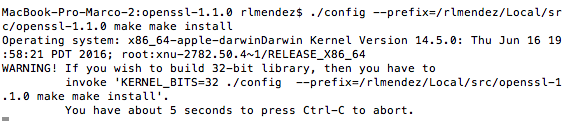
\includegraphics[scale=0.5]{openssl/4_OpenSSL}.\end{center}} & Compilar e instalar. \\ \hline
%{\begin{center}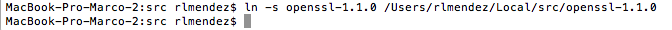
\includegraphics[scale=0.45]{openssl/5_OpenSSL}.\end{center}} & Crear un vínculo simbólico que apunte a la Librería. \\ \hline
%{\begin{center}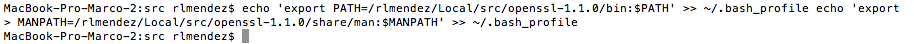
\includegraphics[scale=0.35]{openssl/6_OpenSSL}.\end{center}} & Actualizar el Bash. \\ \hline
%{\begin{center}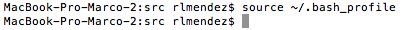
\includegraphics[scale=0.6]{openssl/7_OpenSSL}.\end{center}} & Cargar las nuevas configuraciones. \\ \hline
%{\begin{center}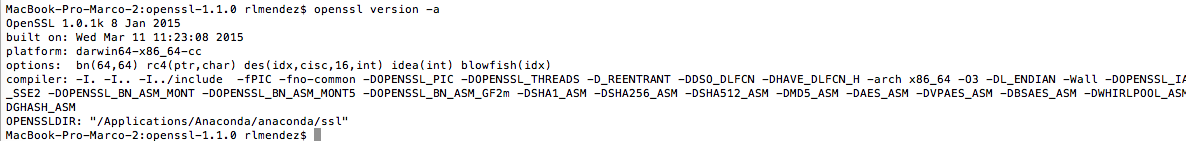
\includegraphics[scale=0.26]{openssl/9_OpenSSL}.\end{center}} & Comprobar la correcta instalación. \\ \hline
%\end{tabular}
%\label{tabla:ConceptosCriptograficos}
%\\\textbf{Fuente:} Propia.
%\end{table}
%   \item Instalación de OpenSSL en otro computador: Explicación de los pasos y con captura de pantallas.
%    \item Ejecución del Protocolo mediante OpenSSL entre los dos computadores: Explicación de los pasos y con captura de pantallas.
%    \item Verificar los resultados: Explicación de los pasos y con captura de pantallas.
%\end{enumerate}

\clearpage

\begin{center}
 \chapter{RESULTADOS}\label{cap.resultados}
\end{center}
\section{Ejecución del Script de Perturbación - Anonimización de Datos}
La ejecución del script permitió la alteración de los datos originales, de esta manera se aplicaron las dos técnicas de anonimización definidas en los lineamientos del Ministerio de Salud y Protección Social. Algunos de los resultados de las ejecuciones del script se observa en las figuras en el cuadro 5.1 donde se evidencian los cambios de algunos valores  después que se  implemento el código de perturbación,  como se señala  en los óvalos rojos.
\begin{table}[h]
\centering
\caption{Datos Originales y Perturbados }
\begin{tabular}{>{\centering\arraybackslash}m{15cm}}
\hline
{\begin{center}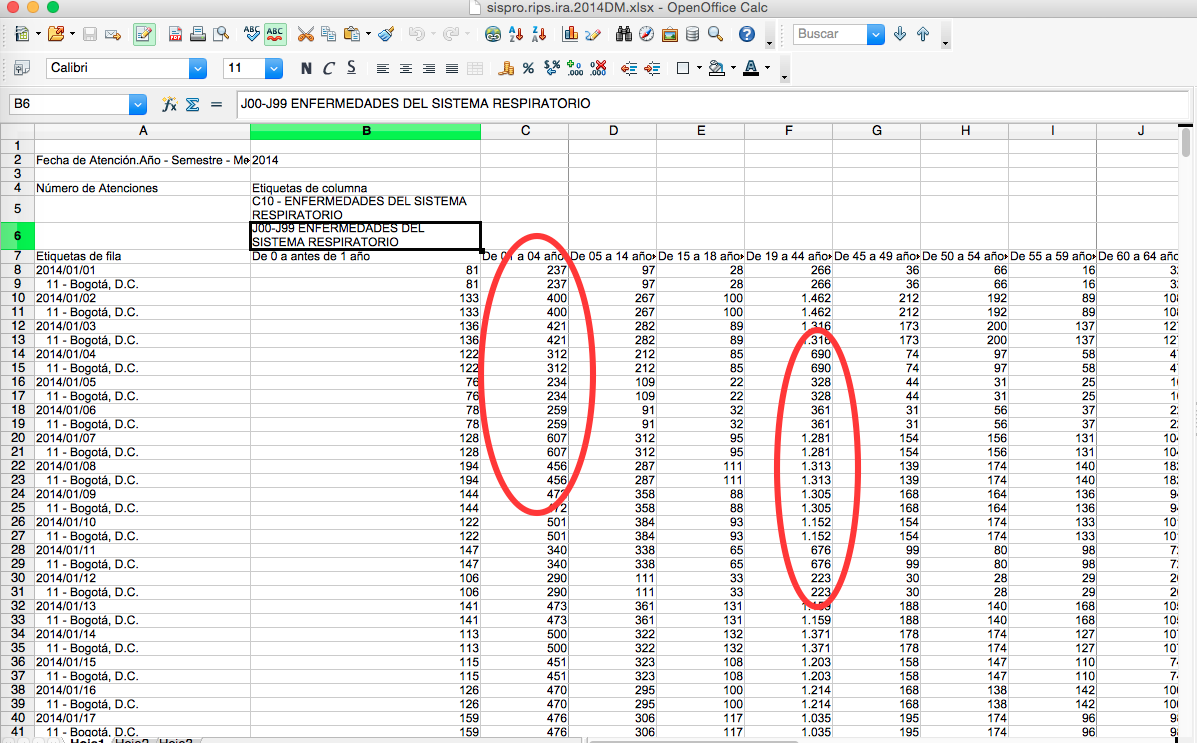
\includegraphics[scale=0.3]{Datos_Originales}.\end{center}} \\ \hline
{\begin{center}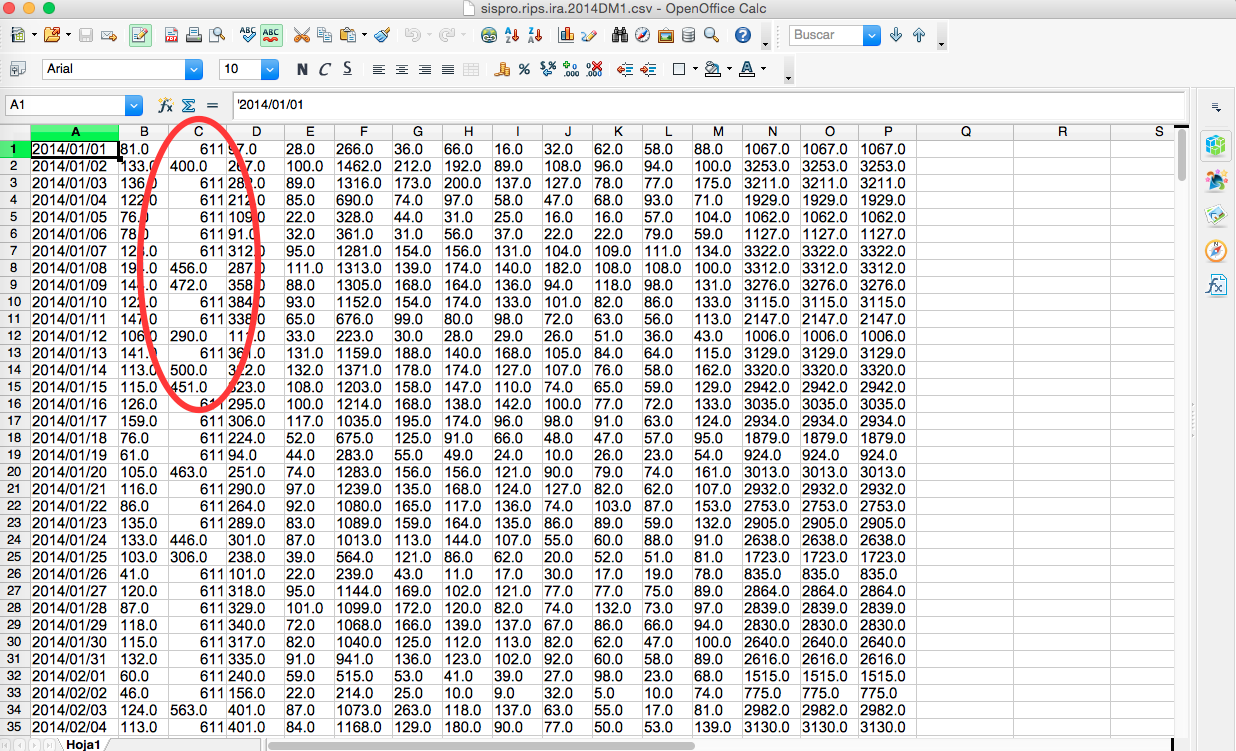
\includegraphics[scale=0.3]{Ejecucion1}.\end{center}} \\ \hline
\end{tabular}
\label{tabla: PerturbadosExperimentoParte1}
\\\textbf{Fuente:} Propia. 
\end{table}
\section{Pre-test \& Pro-test}
El análisis de la información de los RIPS, será dado por los rangos de edades extremos (los primeros y últimos años de vida). De esta manera se realiza una comparación entre  los datos originales (Parte superior) con la ejecución del script, donde se aplicó sobre las mismas columnas (la columna de 0 a 1 años, 1 a 4 años, 70 a 74 años y 75 o más años) y utilizando dos técnicas diferentes permutación y microagregación (Intermedia e Inferior) Cuadros 5.6, 5.7, 5.8 y 5.9 .\\\\Se tuvieron en cuenta las características de probabilidades, para evidenciar también los cambios generados con las técnicas de anonimización. Para el cuadro 5.2, respecto a los datos de la columna de los rangos de 0 a 1 años, la técnica de permutación conservo los mismos valores estadísticos de la información original solo variando la distribución espacial en la gráfica, mientras que la microagregación fue menor la dispersión de los datos según Cuadro. 5.6 pero varia muy poco en el valor mínimo y promedio, disminuyendo la desviación una diferencia pequeña. Para los rangos de 1 a 4 años, sucedió el mismo evento del rango anterior, donde disminuye muy poco el promedio, aumenta en dos números el valor mínimo y al mismo tiempo la dispersión es menor cuando se aplicó la microagregación a los datos, pero la distribución espacial de los puntos en la gráfica si varia respecto a la original según Cuadro 5.7.\\\\ En el cuadro 5.4. de los rangos de 70 a 74 años, la perturbación con la permutación y microagregación, genero los mismos valores estadísticos del estudio con la distribución en la gráfica muy similar pero clasificando en diferentes clustering los valores dados, lo que demuestra que a pesar de la igualdad en lo anterior los valores particulares son diferentes como se evidencia en el cuadro 5.8. En el cuadro 5.5 de los rangos finales desde los 75 años para adelante, nuevamente la permutación sigue preservando las características de probabilidad mencionadas y la microagregación conserva una de los cuatro (valor mínimo) con una dispersión menor respecto a los originales y permutados, gráficamente se puede comparar en el cuadro 5.9.\\\\La disminución con poca diferencia respecto a la original de las desviaciones en las cuatro columnas, permite entender que el proceso de microagregación normaliza los valores dentro de los rangos de la información original y acercándose a si mismo al promedio original.  
\begin{table}[!ht]
\centering
\caption{Estadísticas de las Minerías de Datos Columna 0 a 1 Años}
\begin{tabular}{>{\centering\arraybackslash}m{2.8cm} >{\arraybackslash}m{2cm}>{\arraybackslash}m{2cm}>{\arraybackslash}m{2cm}>{\arraybackslash}m{2cm} }
\hline
\textbf{\textit{Proceso}} & \textbf{\textit{Valor Mínimo}} & \textbf{\textit{Valor Máximo}}& \textbf{\textit{Promedio}}& \textbf{\textit{Desviación}}\\ \hline
Originales & 41 & 415 & 185.8 & 76.08 \\ \hline
Permutados & 41 & 415 & 185.8 & 76.08 \\ \hline
Microagregación & 42.5 & 399.5 & 185.3 & 75.82 \\ \hline
\end{tabular}
\label{tabla:ConceptosCriptograficos}
\\\textbf{Fuente:} Propia.
\end{table}
\begin{table}[!ht]
\centering
\caption{Estadísticas de las Minerías de Datos Columna 1 a 4 Años}
\begin{tabular}{>{\centering\arraybackslash}m{2.8cm} >{\arraybackslash}m{2cm}>{\arraybackslash}m{2cm}>{\arraybackslash}m{2cm}>{\arraybackslash}m{2cm} }
\hline
\textbf{\textit{Proceso}} & \textbf{\textit{Valor Mínimo}} & \textbf{\textit{Valor Máximo}}& \textbf{\textit{Promedio}}& \textbf{\textit{Desviación}}\\ \hline
Originales & 157 & 1918 & 681.5 & 355.11 \\ \hline
Permutados & 157 & 1918 & 681.5 & 355.11 \\ \hline
Microagregación & 159 & 1690 & 680.8 & 351.85 \\ \hline
\end{tabular}
\label{tabla:ConceptosCriptograficos}
\\\textbf{Fuente:} Propia.
\end{table}
\begin{table}[!ht]
\centering
\caption{Estadísticas de las Minerías de Datos Columna 70 a 74 Años}
\begin{tabular}{>{\centering\arraybackslash}m{2.8cm} >{\arraybackslash}m{2cm}>{\arraybackslash}m{2cm}>{\arraybackslash}m{2cm}>{\arraybackslash}m{2cm} }
\hline
\textbf{\textit{Proceso}} & \textbf{\textit{Valor Mínimo}} & \textbf{\textit{Valor Máximo}}& \textbf{\textit{Promedio}}& \textbf{\textit{Desviación}}\\ \hline
Originales & 2 & 111 & 43.7 & 21.4 \\ \hline
Permutados & 2 & 111 & 43.7 & 21.4 \\ \hline
Microagregación & 2 & 111 & 43.7 & 21.4 \\ \hline
\end{tabular}
\label{tabla:ConceptosCriptograficos}
\\\textbf{Fuente:} Propia.
\end{table}
\begin{table}[!ht]
\centering
\caption{Estadísticas de las Minerías de Datos Columna 75 o más Años}
\begin{tabular}{>{\centering\arraybackslash}m{2.8cm} >{\arraybackslash}m{2cm}>{\arraybackslash}m{2cm}>{\arraybackslash}m{2cm}>{\arraybackslash}m{2cm} }
\hline
\textbf{\textit{Proceso}} & \textbf{\textit{Valor Mínimo}} & \textbf{\textit{Valor Máximo}}& \textbf{\textit{Promedio}}& \textbf{\textit{Desviación}}\\ \hline
Originales & 20 & 223 & 91.4 & 39.09 \\ \hline
Permutados & 20 & 223 & 91.4 & 36.09 \\ \hline
Microagregación & 20 & 206 & 91.2 & 35.72 \\ \hline
\end{tabular}
\label{tabla:ConceptosCriptograficos}
\\\textbf{Fuente:} Propia.
\end{table}

\begin{table}[h]
\centering
\caption{Datos Originales (Parte Superior), Anonimizados Permutación (Parte Intermedia) y Anonimizados Microagregación (Parte Inferior)  para 0 a 1 años}
\begin{tabular}{>{\centering\arraybackslash}m{15cm}}
\hline
{\begin{center}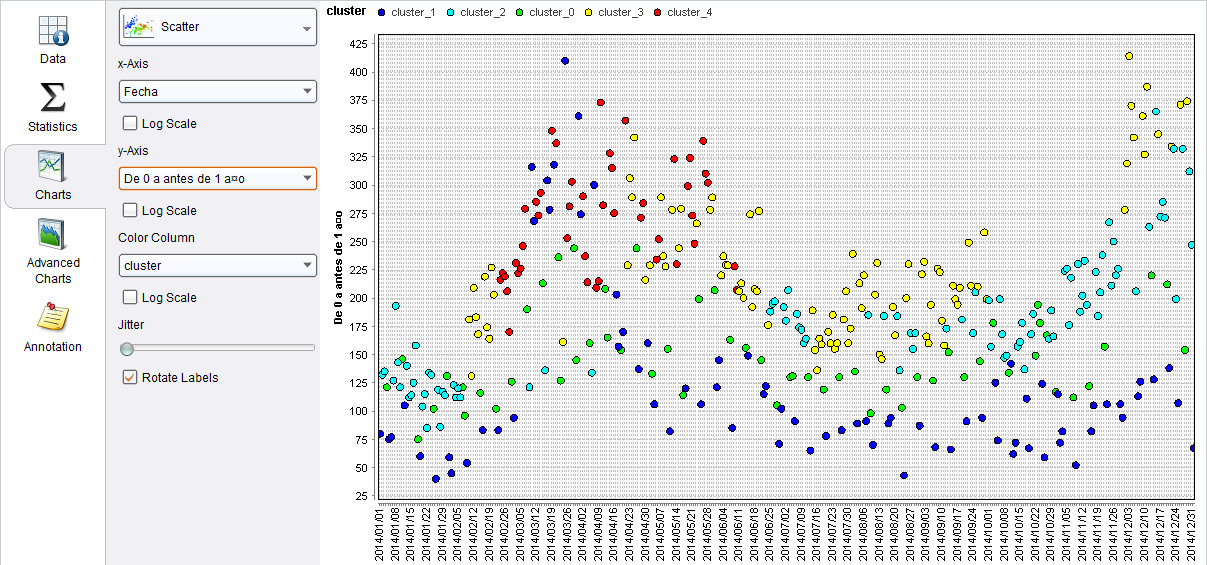
\includegraphics[scale=0.36]{EjecucionO/EjecucionO_0_1}.\end{center}} \\ \hline
{\begin{center}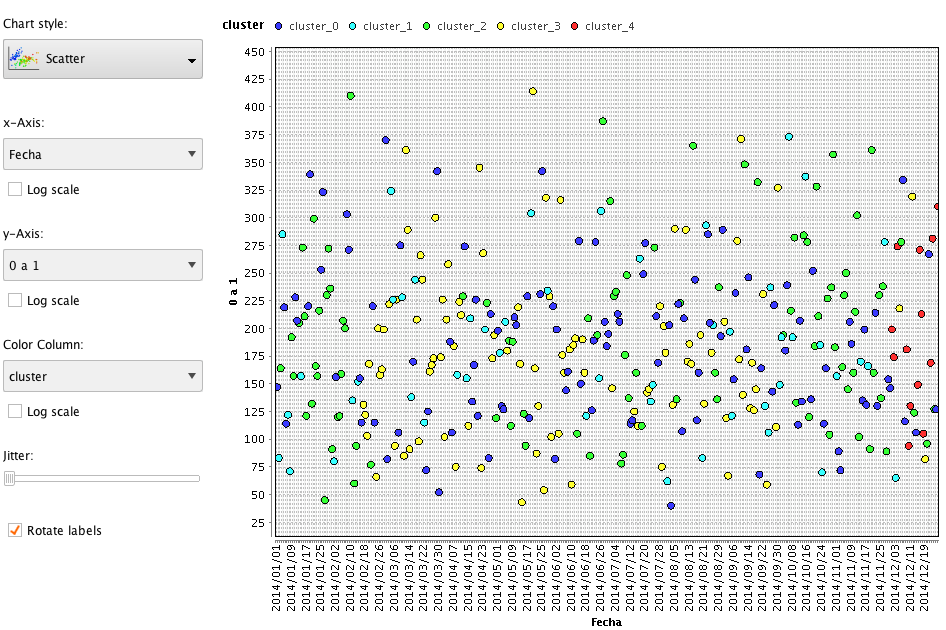
\includegraphics[scale=0.28]{Permutacion/0-1_Permutacion}.\end{center}} \\ \hline
{\begin{center}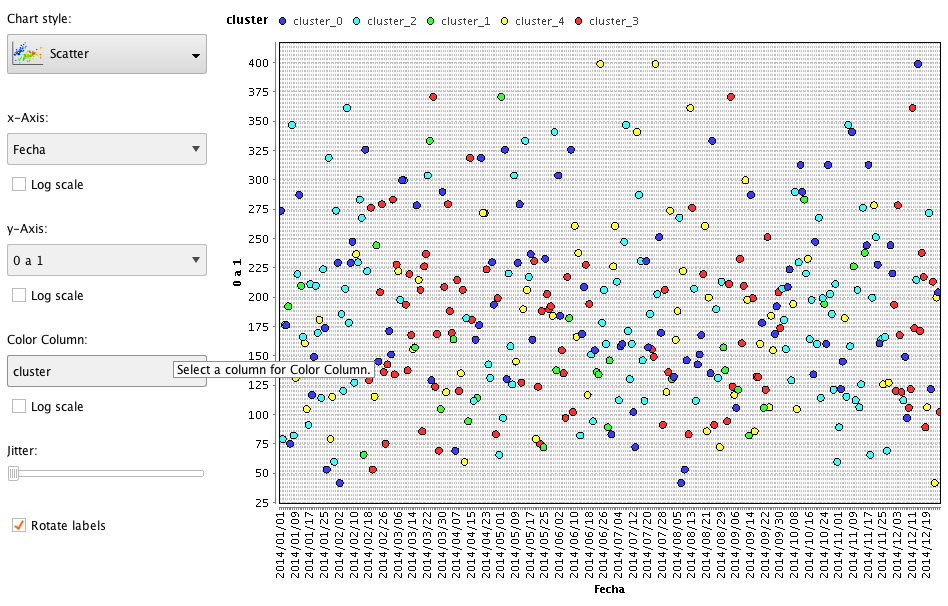
\includegraphics[scale=0.28]{Micro/0-1_Micro}.\end{center}} \\ \hline
\end{tabular}
\label{tabla: PerturbadosExperimentoParte1}
\\\textbf{Fuente:} Propia.
\end{table}
\begin{table}[h]
\centering
\caption{Datos Originales (Parte Superior), Anonimizados Permutación (Parte Intermedia) y Anonimizados Microagregación (Parte Inferior)  para 1 a 4 años}
\begin{tabular}{>{\centering\arraybackslash}m{15cm}}
\hline
{\begin{center}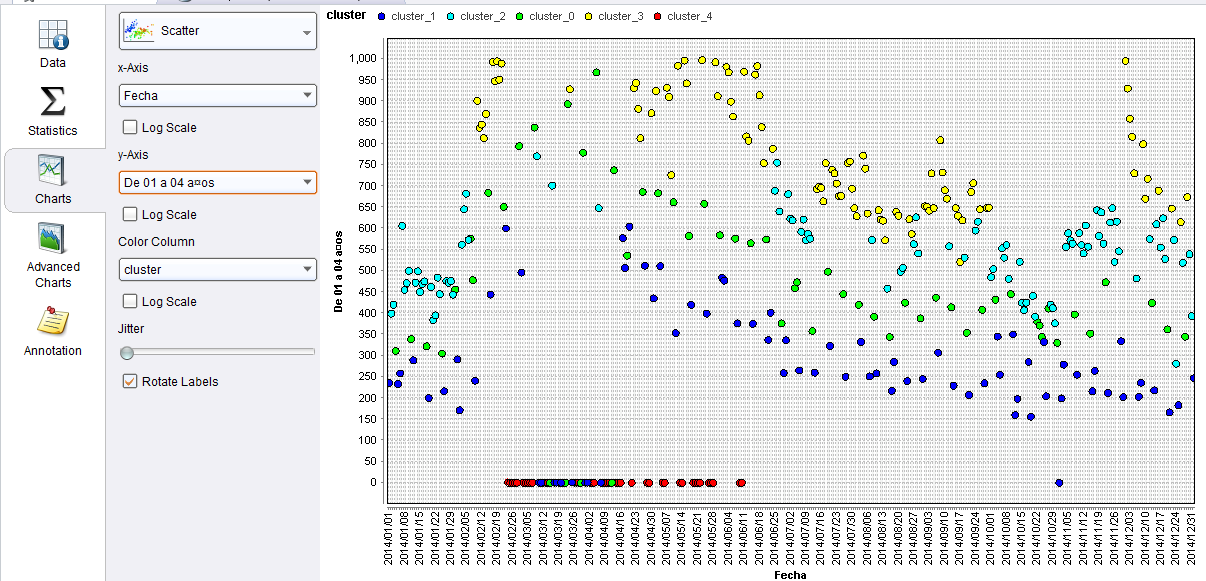
\includegraphics[scale=0.36]{EjecucionO/EjecucionO_1_4}.\end{center}} \\ \hline
{\begin{center}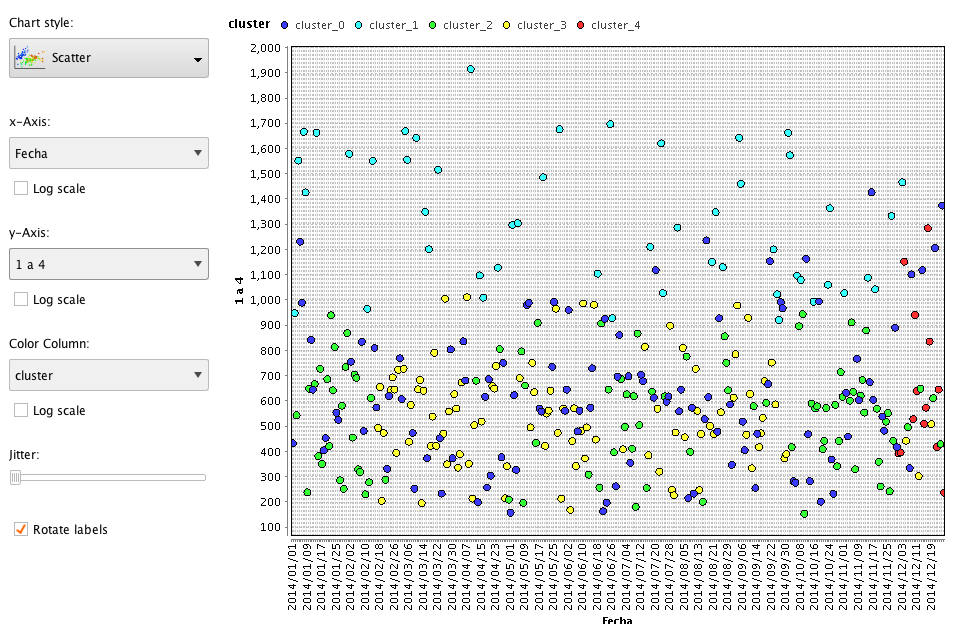
\includegraphics[scale=0.28]{Permutacion/1-4_Permutacion}.\end{center}} \\ \hline
{\begin{center}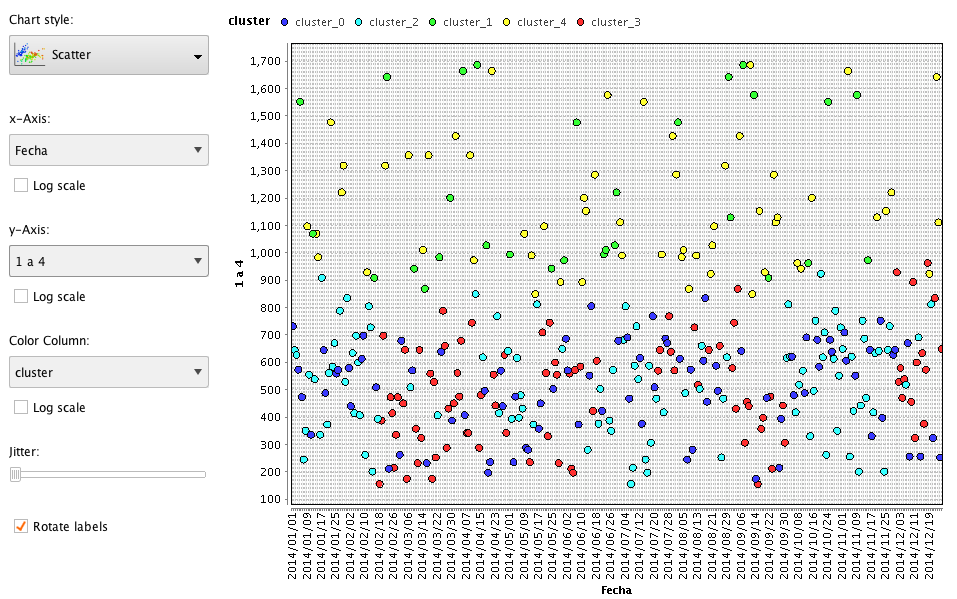
\includegraphics[scale=0.28]{Micro/1-4_Micro}.\end{center}} \\ \hline
\end{tabular}
\label{tabla: PerturbadosExperimentoParte1}
\\\textbf{Fuente:} Propia.
\end{table}
\begin{table}[h]
\centering
\caption{Datos Originales (Parte Superior), Anonimizados Permutación (Parte Intermedia) y Anonimizados Microagregación (Parte Inferior)  para 70 a 74 años}
\begin{tabular}{>{\centering\arraybackslash}m{15cm}}                   \hline
{\begin{center}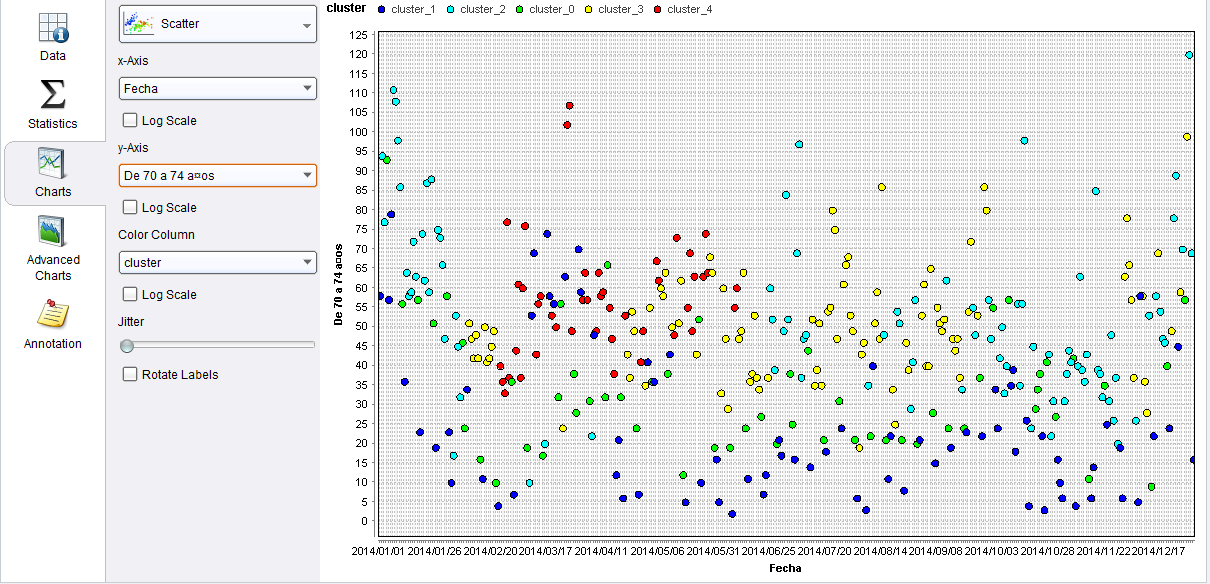
\includegraphics[scale=0.36]{EjecucionO/EjecucionO_70_74}.\end{center}} \\ \hline
{\begin{center}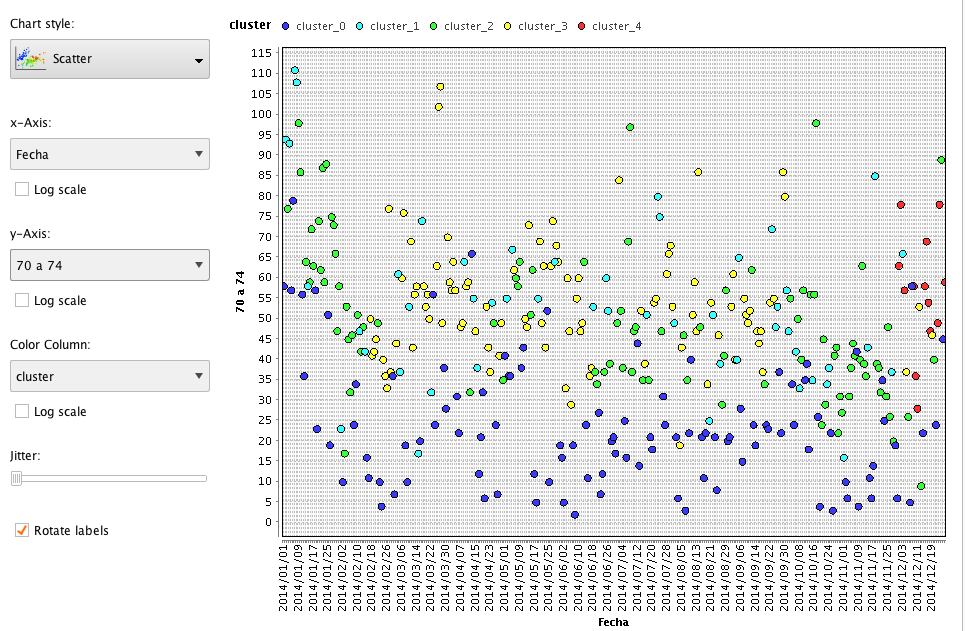
\includegraphics[scale=0.28]{Permutacion/70-74_Permutacion}.\end{center}} \\ \hline
{\begin{center}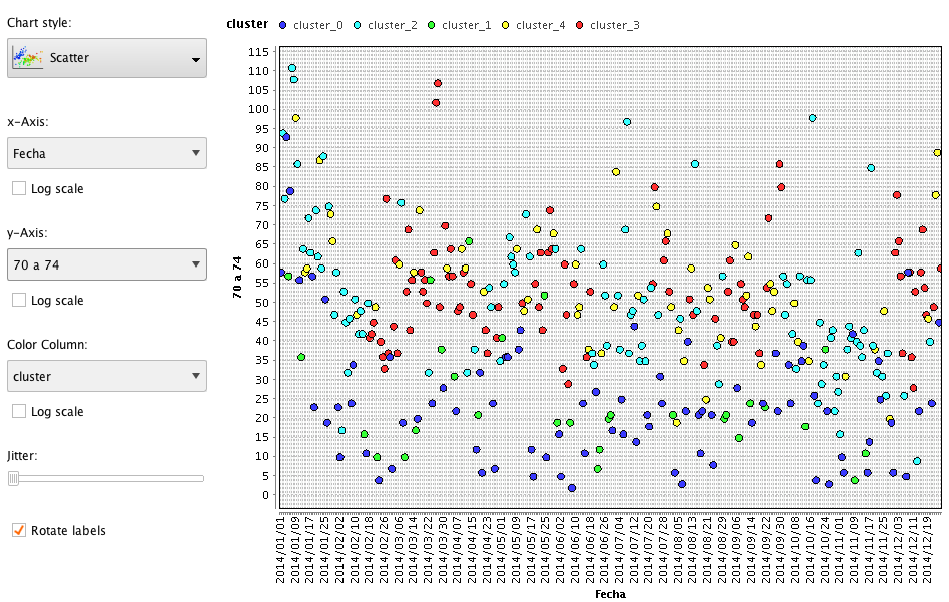
\includegraphics[scale=0.28]{Micro/70-74_Micro}.\end{center}} \\ \hline
\end{tabular}
\label{tabla: PerturbadosExperimentoParte1}
\\\textbf{Fuente:} Propia.
\end{table}
\begin{table}[h]
\centering
\caption{Datos Originales (Parte Superior), Anonimizados Permutación (Parte Intermedia) y Anonimizados Microagregación (Parte Inferior)  para 75 a más años}
\begin{tabular}{>{\centering\arraybackslash}m{15cm}}
\hline
{\begin{center}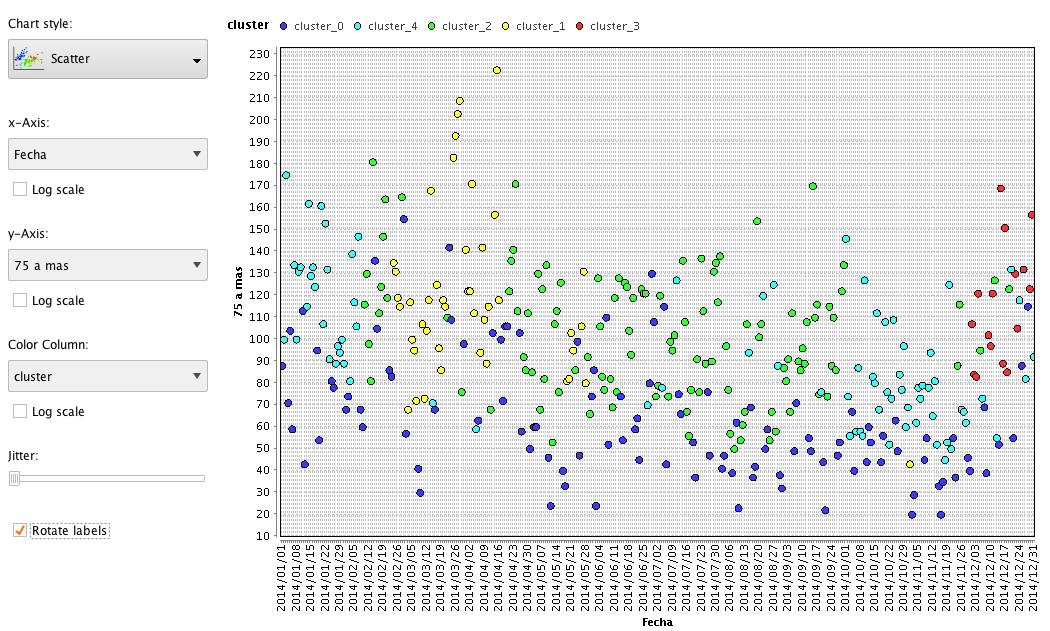
\includegraphics[scale=0.29]{EjecucionO/75_a_mas_Originales}.\end{center}} \\ \hline
{\begin{center}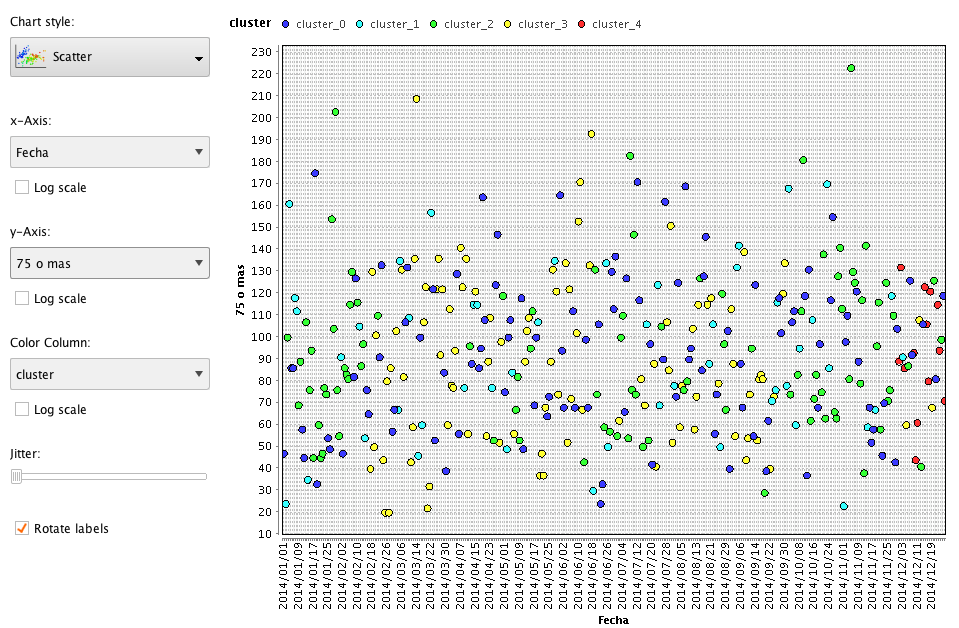
\includegraphics[scale=0.25]{Permutacion/75_o_mas_Permutacion}.\end{center}} \\ \hline
{\begin{center}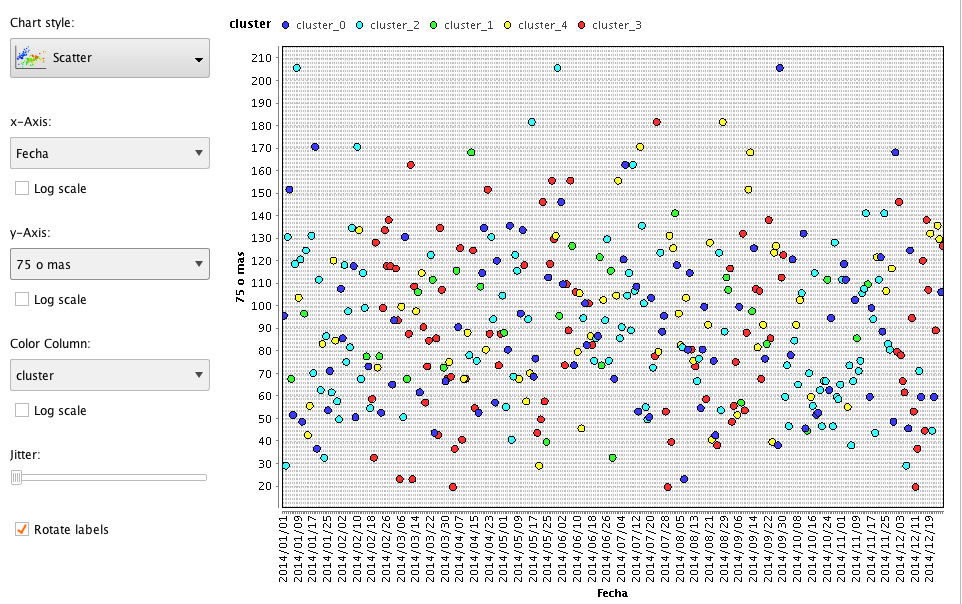
\includegraphics[scale=0.25]{Micro/75_o_mas_Micro}.\end{center}} \\ \hline
\end{tabular}
\label{tabla: PerturbadosExperimentoParte1}
\\\textbf{Fuente:} Propia.
\end{table}

\begin{center}
 \chapter{ANÁLISIS}\label{cap.analisis}
\end{center}
\section{Análisis Técnico de la Minería de Datos}
Después de evidenciar los resultados reportados en las dos técnicas de anonimización de los datos RIPS, la técnica que mejor realiza el proceso de perturbar los datos originales es la técnica de Permutación, ya que en las cuatros columnas de los diferentes rangos de edad escogidas preservo el 95\% de las características estudiadas (valor mínimo, valor máximo, promedio, desviación) frente a un 55\% de la preservación de las variables nombradas, en todas preservo el valor máximo pero en su totalidad las otras.\\\\
De la microagregación frente a los datos originales y permutación, fue moda que el valor mínimo estuviera más alto, junto con el promedio, pero siendo la desviación menor (excepto en la ejecución de la columna 70 a 74 años que fue igual en las cuatro variables). Estos resultados son respaldados por los Lineamientos del Ministerio de Salud y Protección Social de Colombia y el DANE, la permutación conservará las estadísticas de los datos, ya que no son alterados pero si ordenados de manera aleatoria, es bueno para el proceso de anonimización porque no se podrá identificar el registro original.En caso de un ataque de fuerza bruta debe probar toda la muestra de la población sin estar seguro del acierto; para la técnica de microagregación por alterar los valores originales pero preservando el rango máximo no puede ser tan exacto al compararse con los originales, aunque la distribución se intente conservar.\\\\Aunque las gráficas tienden a ser diferentes visualmente entre los datos originales frente a los dos procesos de anomización, los resultados pueden ser próximos a los originales  estadísticamente se conserva la información aunque los valores individuales hayan cambiado. Resaltando que la desviación es un indicador recalca que la información se aproxima a la media con menor dispersión, causado por la distribución y estandarizado de los datos (micro agregación).

\section{Análisis Resultados Minería de Datos}
De las trece estaciones de monitoreo ubicadas en la ciudad de Bogotá, para una sección de la investigación se realizó la minería de los datos de tres estaciones de monitoreo de las trece que conforman la RMCAB.\\\\Puente Aranda y Kennedy históricamente son localidades industriales y comerciales de la capital colombiana según las Figuras 6.1, 6.2 y 6.3 que son algunos sectores de la industria que existen. En las figuras 6.4, 6.5 y 6.6 es notable la alta concentración de SO2, NO2 y CO en la estación de monitoreo de Puente Aranda, después le sigue la estación de Kennedy con los mismos componentes y finalmente Carvajal posiblemente por las actividades  relacionadas en las figuras anteriores.\\\\El SO2 tiene propiedades desinfectantes, conservantes y materia prima de detergentes, este compuesto es un gas irritante y tóxico, el cual puede irritar el tracto respiratorio, causar bronquitis y congestionar los conductos bronquiales de los asmáticos complicaciones clasificadas de las IRA. El NO2 es producido en procesos de combustión a altas temperaturas, como en los vehículos motorizados y las plantas eléctricas, es acertado por el porcentaje de empresas dedicadas a la transformación de productos y usos automotriz, además por la maquinaria deben tener plantas eléctricas de respaldo para su producción, este compuesto afecta el sistema respiratorio, a corto plazo en altos niveles causa daños en las células pulmonares, mientras a largo plazo en niveles bajos  puede causar cambios irreversibles en el tejido pulmonar. Finalmente para el CO es producido en la combustión deficiente de sustancias como gas, gasolina, petróleo, tabaco o madera; este gas es muy peligroso por su alto nivel de toxicidad ya que solamente exponerse un lapso corto puede causar vomito, desmayo y diarrea hasta la muerte.\\\\

\begin{figure}[!ht]
\centering
\caption{Eslabones y distribución de las empresas de la cadena de metalmecánica. Puente Aranda}
 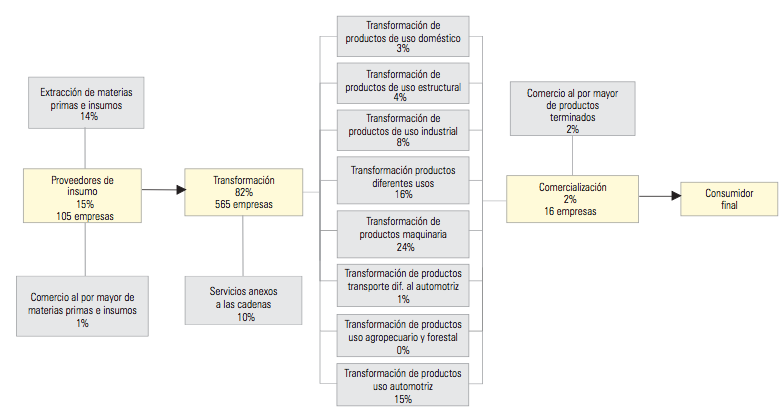
\includegraphics[scale=0.55]{Puente}
\label{fig:1_OpenSSL}
\\ \textbf{Fuente:} CB (2006). Registro mercantil. Cámara de Comercio de Bogotá. Proceso: Dirección de Estudios e Investigaciones de la CCB.
\end{figure}
\begin{figure}[!ht]
\centering
\caption{Eslabones y distribución de las empresas de la cadena de productos alimenticios.Puente Aranda}
 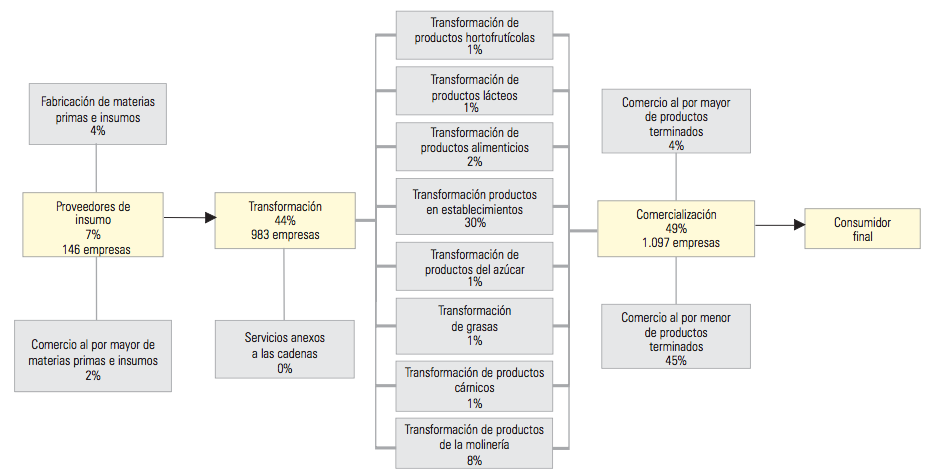
\includegraphics[scale=0.5]{Puente2}
\label{fig:1_OpenSSL}
\\ \textbf{Fuente:} CB (2006). Registro mercantil. Cámara de Comercio de Bogotá. Proceso: Dirección de Estudios e Investigaciones de la CCB.
\end{figure}
\begin{figure}[!ht]
\centering
\caption{Número de empresas en Kennedy según sector económico y tamaño. Kennedy}
 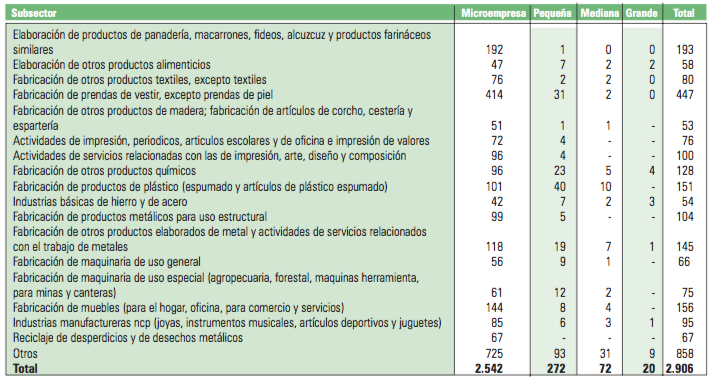
\includegraphics[scale=0.6]{Kennedy}
\label{fig:1_OpenSSL}
\\ \textbf{Fuente:} Registro Mercantil. Cámara de Comercio de Bogotá, 2004. Proceso: Dirección de Estudios e Investigaciones de la CCB.
\end{figure}
 
\begin{figure}[ht]
\centering
\caption{Concentración de Dióxido de Azufre SO2 RMCAB Carvajal (Azul), Kennedy (Verde) y Puente Aranda (Rojo)}
 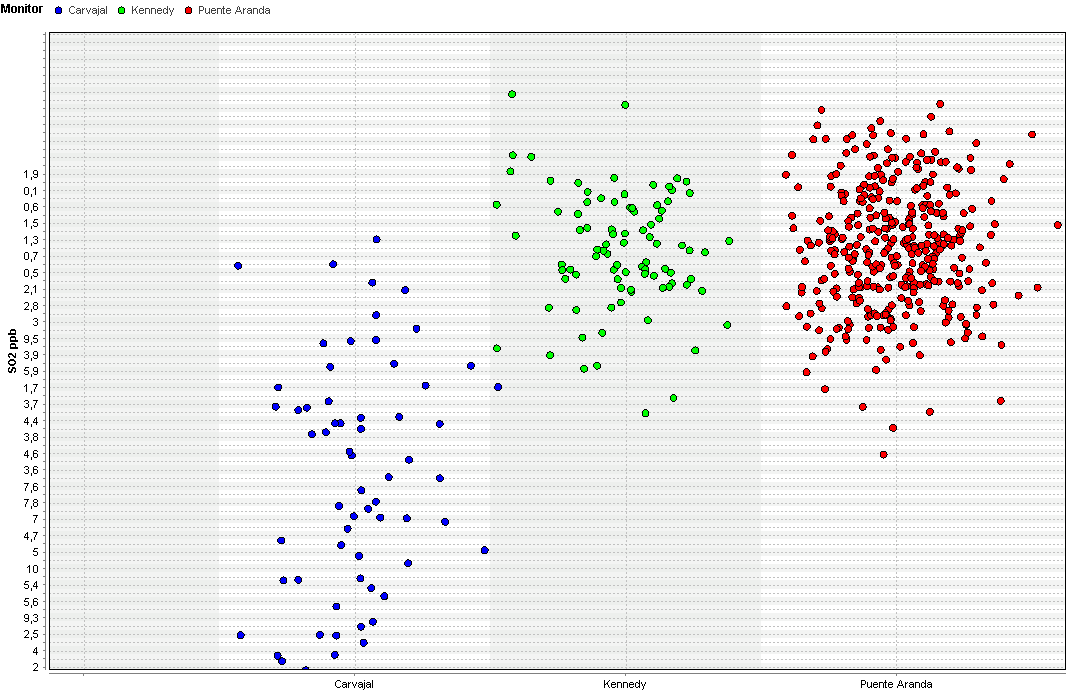
\includegraphics[scale=0.45]{RMCABanalisis/AnalisisRMCABSO2}
\label{fig:1_OpenSSL}
\\ \textbf{Fuente:} Propia.
\end{figure}

\begin{figure}[h]
\centering
\caption{Concentración de Dióxido de Nitrógeno NO2 RMCAB Carvajal (Azul), Kennedy (Verde) y Puente Aranda (Rojo)} 
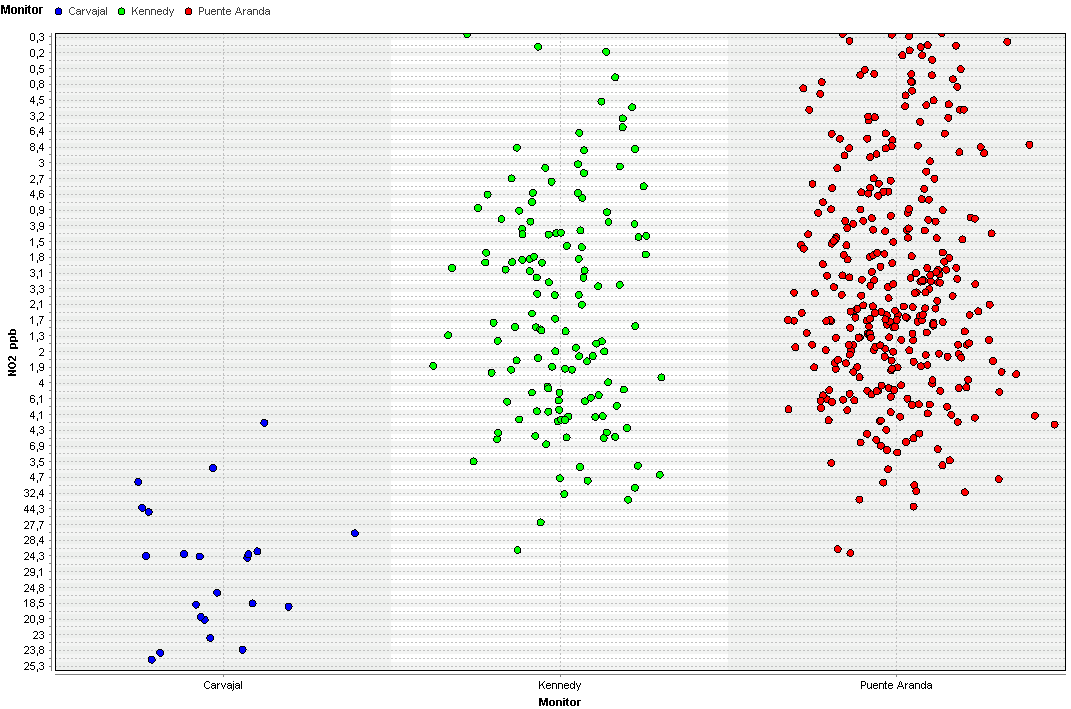
\includegraphics[scale=0.45]{RMCABanalisis/AnalisisRMCABNO2}
\label{fig:Tabla1}
\\ \textbf{Fuente: }Propia.
\end{figure}

\begin{figure}[h]
\centering
\caption{Concentración de Monóxido de Carbono CO RMCAB Carvajal (Azul), Kennedy (Verde) y Puente Aranda (Rojo)} 
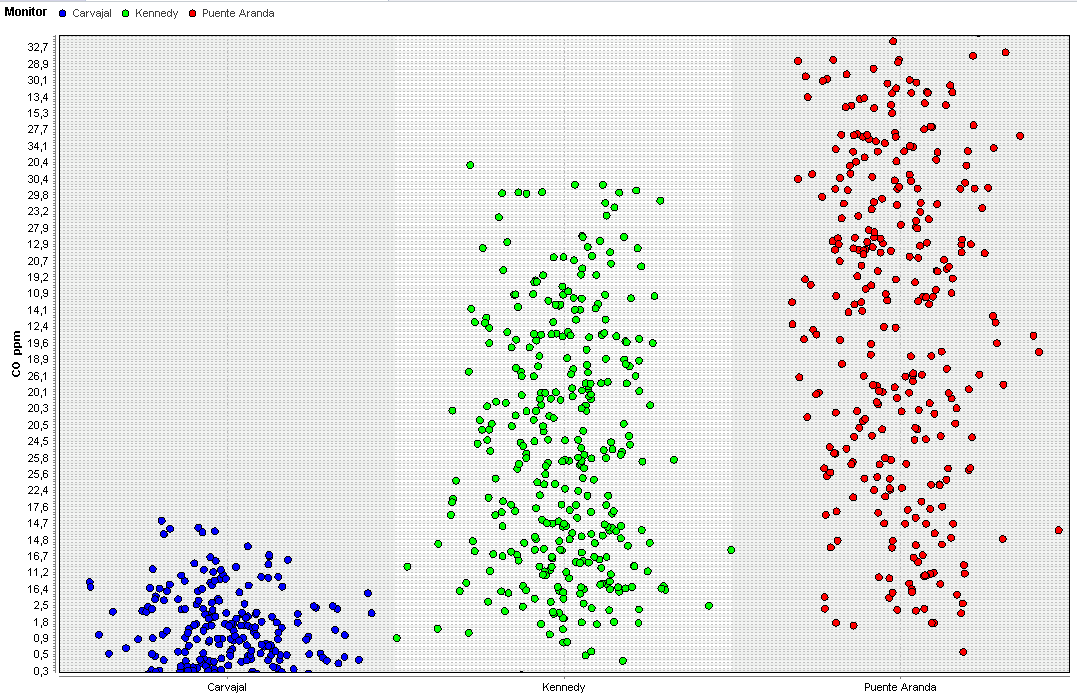
\includegraphics[scale=0.45]{RMCABanalisis/AnalisisRMCABCO}
\label{fig:Tabla1}
\\ \textbf{Fuente: }Propia.
\end{figure}
Ahora respecto a la información de todas las estaciones de monitoreo y los registros de RIPS, tomando como referencia las estaciones de Carvajal, Puente Aranda y Kenedy se puede evidencia de manera particular que:
\begin{enumerate}
	\item \textbf{Puente Aranda:} En la figura 6.7 se evidencia que los niveles más altos de los componentes contaminante, es NO2 se comporta de manera creciente respecto a CO y SO2, pero en el instante de relacionarse con los rangos de edades de 0 a 1 años y 1 a 4 años, se puede evidencia que los valores de mayores atenciones se registran cuando el NO2 esta en los rangos de 25 ppb a 27 ppb pero los otros rangos se encuentran en los valores cercanos a la media, también se evidencia que se registran en los meses de febrero y marzo, cuando algunos infantes ya comienzan a ser dejados en jardines o expuestos más seguido al ambiente. Para las columnas de 70 a 74 años y más de 75 años, sucede lo mismo se disparan el número de atenciones cuando el NO2 se encuentra en los mismos rangos mencionados.
    \item \textbf{Kennedy:} En la figura 6.8 se evidencia que el NO2 tiende a tener los valores más altos, pero en los rangos de 0 a 1 años y 1 a 4 años la afectación se ve reflejado en los puntos máximos el NO2 y SO2 en marzo y diciembre. Pero en los rangos de 70 a 74 años y 55 o más años, se da en abril y diciembre cuando el NO2 alcanza valores altos de emisión.
    \item \textbf{Carvajal:} En la figura 6.9 se evidencia que los niveles más altos de los componentes contaminante, es NO2 el cual se distribuye de  manera similar en el transcurso de los días y superando los otros dos componentes. Pero en los rangos de 0 a 1 años y 1 a 4 años, se registran los puntos más altos de atenciones cuando el CO sobre pasa a los otros dos componentes, este evento sucede en los meses de marzo y diciembre. Para los rangos de 70 a 74 años y más de 75 años tiende a comportarse de la misma manera del evento anterior.
\end{enumerate}

\begin{figure}[h]
\centering
\caption{Comportamiento de SO2, NO2 y CO Puente Aranda} 
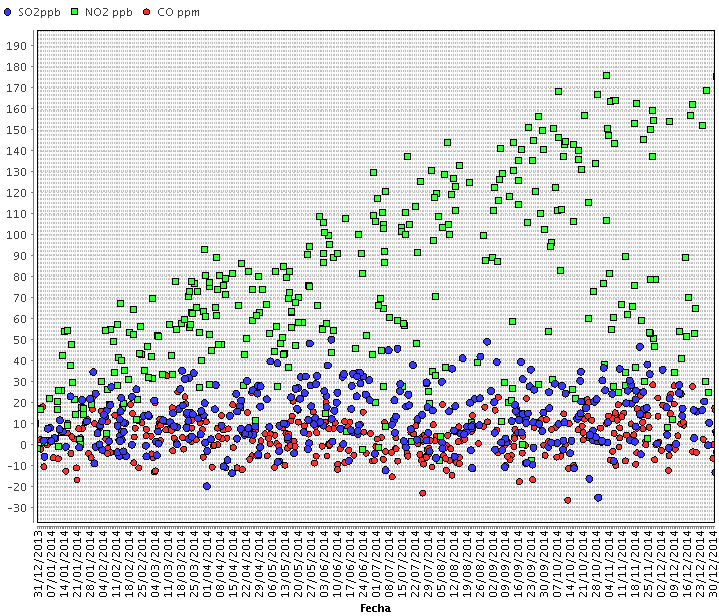
\includegraphics[scale=0.47]{Componentes/Puente_Aranda_Componentes}
\label{fig:Tabla1}
\\ \textbf{Fuente: }Propia.
\end{figure}
\begin{figure}[h]
\centering
\caption{Comportamiento de SO2, NO2 y C0 Kenedy} 
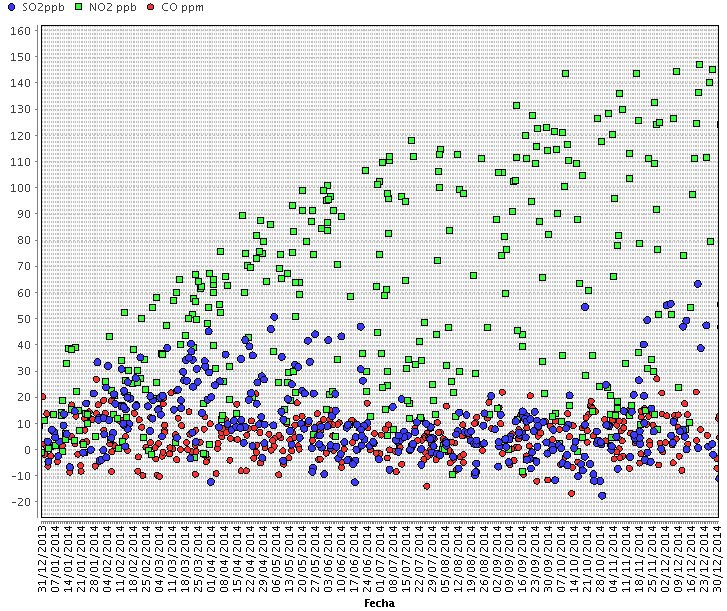
\includegraphics[scale=0.47]{Componentes/Kenedy_Componentes}
\label{fig:Tabla1}
\\ \textbf{Fuente: }Propia.
\end{figure}
\begin{figure}[h]
\centering
\caption{Comportamiento de SO2, NO2 y C0 Carvajal} 
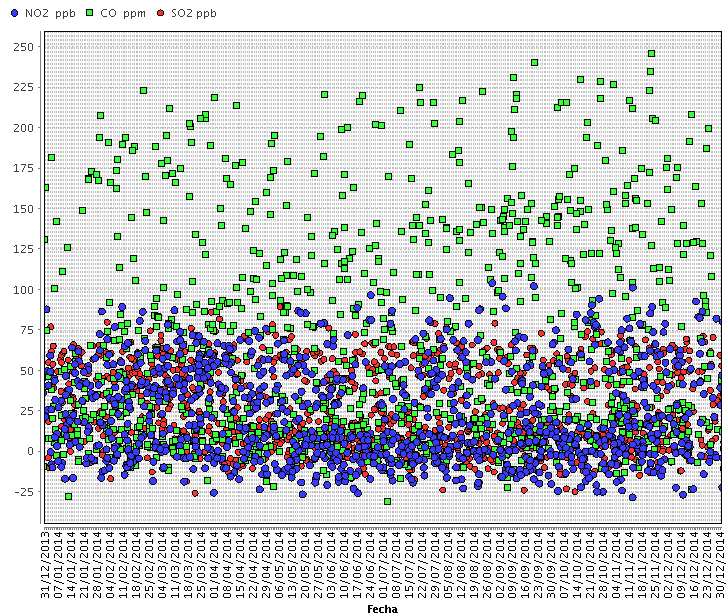
\includegraphics[scale=0.47]{Componentes/Carvajal_Componentes}
\label{fig:Tabla1}
\\ \textbf{Fuente: }Propia.
\end{figure}


\begin{center}
 \chapter{CONCLUSIONES Y RECOMENDACIONES}\label{cap.conclusiones}
\end{center}

\section{Conclusiones}

Al realizar la minería de datos con la información anonimizada y compararlos con los datos originales, se evidencio que las técnicas de permutación y microagregación realizaron cambios en los datos en su distribución pero preservando o aproximándose las características estadísticas (promedio, valor mínimo, valor máximo y desviación), lo que demuestra que se puede realizar un análisis con la confianza que los datos anonimizados se acercan a la realidad, desafortunadamente no se puedo contar con información de String para comprender su comportamiento al aplicar otra técnica acorde al tipo de variable, siendo una recomendación para investigaciones futuras. Aún así es importante resaltar que la simulación de los procesos de minería de datos fue efectivo asumiendo que los dos proveedores ejecutaron una técnica diferente (permutación o microagregación) para tener resultados próximos a la información original.\\\\  La clasificación implementando el algoritmo clustering permitió agrupar la información en cinco grupos referente a los rangos de edades dados en los RIPS para confrontarse con los tres grupos de los compuestos NO2, SO2 y CO para interpretar las posibles relaciones.\\\\Respecto a los mecanismos implementados para la anonimización fue crucial entender que en las técnicas seleccionadas y aplicadas, la información de tipo númerico se puede evidenciar que los datos se afectaron pero la información, la interpretación puede ser aproximada a la original, variando ya los cambios que se tuvieron en los valores mínimos y desviaciones en el caso de la microagregación, lo que es una buen resultado del código implementando en Python para aplicar la perturbación de los datos. Esta arquitectura o diseño fue apropiada con la información obtenida de las tres fuentes, pero se debe entender que cada día los datos pueden variar y así mismo las necesidades de las entidades,  lo cual de la arquitectura propuesta se puede aplicar el método pero cambiando posiblemente los procesos de minería de datos junto con las técnicas de anonimización.\\\\Concluyendo que los procesos de anonimización de los datos son efectivos en datos númericos, ya que en otros tipos de variables no se pudo evidenciar por su inexistencia dentro de los datos e investigación.
\section{Recomendaciones}
Algunas recomendaciones de la investigación teniendo en cuenta los resultados e inconvenientes, se sugiere para próximos desarrollos o investigaciones los siguientes temas:
\begin{enumerate}
	\item Recuperación de los datos originales por parte de un minero, aplicando procesos estadísticos a información perturbada.
    \item Aplicar otras técnicas de anonimización acordes a variables tipo String, para comprender e interpretar los comportamientos de las mismas para realizar cualquier proceso de minería de datos requeridos.
    \item AGREGAR LA PROPUESRA DE LA ARQUTECTUA DEL ARTICULO !!!!! PEDIRLO AL ING DAVID URG
\end{enumerate}
\clearpage

\begin{center}
 \chapter{GLOSARIO DE TÉRMINOS}\label{cap.glosario}
\end{center}
AGENTES ETIOLOGICOS: el agente etiologico es el que causa la enfermedad. el agente transmisor es el que lo transmite de un organismo a otra.\\\\
ALGORITMO: es un conjunto prescrito de instrucciones o reglas bien definidas, ordenadas y finitas que permite realizar una actividad mediante pasos sucesivos. \\\\
ANONIMIZAR: es la necesidad de los cibernautas de ocultar información mientras navegan para evitar el uso de sus datos personales (como la dirección IP o la situación geográfica) con fines estadísticos, publicitarios o vandálicos ha causado la aparición del neologismo anonimizar, que se ha extendido después a otros ámbitos.  \\\\
DATASETS: es una colección de datos habitualmente tabulada.En general y en su versión más simple, un conjunto de datos corresponde a los contenidos de una única tabla de base de datos o una única matriz de datos estadística, donde cada columna de la tabla representa una variable en particular, y cada fila representa a un miembro determinado del conjunto de datos en cuestión. Un conjunto de datos contiene los valores para cada una de las variables, como por ejemplo la altura y el peso de un objeto, que corresponden a cada miembro del conjunto de datos. Cada uno de estos valores se conoce con el nombre de dato. El conjunto de datos puede incluir datos para uno o más miembros en función de su número de filas.\\\\
ENCRIPTACIÓN: es el proceso para volver ilegible información considera importante. La información una vez encriptada sólo puede leerse aplicándole una clave. Se trata de una medida de seguridad que es usada para almacenar o transferir información delicada que no debería ser accesible a terceros.\\\\
INFECCIÓN DE RESPIRACIÓN AGUDA: la Infección Respiratoria Aguda (IRA) constituyen un grupo de enfermedades que se producen en el aparato respiratorio, causadas por diferentes microorganismos como virus y bacterias, que comienzan de forma repentina y duran menos de 2 semanas.
La mayoría de estas infecciones como el resfriado común son leves, pero dependiendo del estado general de la persona pueden complicarse y llegar a amenazar la vida, como en el caso de las neumonías. \\\\
INFORMACIÓN SENSIBLE: Es la información que debe ser estrictamente protegida, ejemplo (edad, dirección, cedula,Fecha de nacimiento, etc).
\\\\
MORBILIDAD:es la proporción de personas (o animales) que se enferman en un sitio y tiempo determinado.1 Minoritariamente también se usa como sinónimo morbilidad, que etimológicamente es correcto.  \\\\
MORTALIDAD:indica el número de fallecimientos de una población en concreto por cada 1000 habitantes, durante un período de tiempo determinado, este puede ser durante un año. \\\\
SCRIPTS: son programas, usualmente pequeños o simples, para realizar generalmente tareas muy específicas. Los scripts son un conjunto de instrucciones generalmente almacenadas en un archivo de texto que deben ser interpretados línea a línea en tiempo real para su ejecución.\\\\
\clearpage

\begin{center}
 \chapter{REFERENCIAS}\label{cap.referencias}
\end{center}

\begin{enumerate}
	\item PLAN DE DESARROLLO INSTITUCIONAL 2013-2016 Versión Enero 2013 del Hospital del Sur.
	\item HERRANZ Javier NIN Jordi Secure and efficient anonymization of distributed confidential databases, Springer-Verlag Berlin Heidelberg 2014, Online: 23 April 2014. Int. J. Inf. Secur. (2014) 13:497–512.
	\item PENCHALAIAH PhD, SESHADRI  PhD. Effective Comparison and Evaluation of DES and Rijndael Algorithm (AES), International Journal on Computer Science and Engineering Vol. 02, No. 05, 2010, 1641-1645.
    \item CORREGIR ESTE ERROR% ÁNGEL A. Juan, SEDANO Máximo, VILA Alicia.} %<http://www.uoc.edu/in3/emath/docs/Distrib_Normal.pdf> [citado en Septiembre 18 del 2016].
    \item M. Berry, G. Linoff, “Mastering data mining: the art andscience of customer relationship management“. West Susex:John Wiley \& Sons, 1999.
    \item DAMGARD Ivan, et at. Multiparty Computation from Somewhat Homomorphic Encryption, International Association for Cryptologic Research 2012, R. Safavi-Naini and R. Canetti (Eds.): CRYPTO 2012, LNCS 7417.
    \item GHODOSI Hossein Ghodosi, et at. Multi-party computation with conversion of secret sharing, Springer Science+Business Media, LLC 2011, Des. Codes Cryptogr. (2012) 62:259–272, Online: 10 May 2011.
    \item KIRAZ SABIR Mehmet, UZUNKOL Osmanbey. Efficient and verifiable algorithms for secure outsourcing of cryptographic computations, Springer-Verlag Berlin Heidelberg 2015, Int. J. Inf. Secur, Online: 15 Nov 2015.
    \item LAUD Peeter. Privacy-Preserving Minimum Spanning Trees through Oblivious Parallel RAM for Secure Multiparty Computation, Online: 25 Nov 2014.
    \item Dirección de Regulación, Planeación, Estandarización y Normalización DIRPEN. Lineamientos para la Anonimización de microdatos VERSIÓN: 01 29-08-2014.
    \item SSL Information and FAQ [En línea] <http://info.ssl.com/article.aspx?id=10241> [citado en 18 de Septiembre del 2016].
    \item Utilizar el protocolo SSL <http://www.4d.com/docs/CMS/CMS02064.HTM> [En línea] [citado en 18 de Septiembre del 2016].
    \item SEJWANI Sapna, TANWAR Sarvesh, Implementation of X.509 Certificate for Online Applications, International Journal of Research in Advent Technology, Vol.2, No.3, March 2014, E-ISSN: 2321-9637.
    \item CELINA Drovandi. CRIPTOGRAFÍA
SEGURIDAD EN ESQUEMAS DE FILE TRANSFER SEGURIDAD EN INTERNET Revista de la Universidad de Mendoza, 2015
    \item Dr. Bhadresh P. Patel, Vishal R. Pancholi. Enhancement of Cloud Computing Security with Secure Data Storage using AES IJIRST –International Journal for Innovative Research in Science and Technology Volume 2 Issue 09 February 2016 ISSN (online): 2349-601.
    \item GOMEZ Vieitis Alvaro. Sistema seguros de acceso y transmisión de datos, RA-MA Editorial.
    \item VELASCO Sánchez Paola Maritza, ANÁLISIS DE LOS MECANISMOS DE ENCRIPTACIÓN PARA LA SEGURIDAD DE LA INFORMACIÓN EN REDES DE COMUNICACIONES, FACULTAD DE INGENIERÍA MAESTRÍA EN REDES DE COMUNICACIONES, PONTIFICIA UNIVERSIDAD CATÓLICA DEL ECUADOR Año 2015
    \item Weiss, S.M. y Indurkhya, N. “Predictive Data Mining. A Practical Guide”Morgan Kaufmann Publishers, San Francisco, 1998.
    \item Cabena, P., Hadjinian, P., Stadler, R., Verhees, J. Y Zanasi, A. “Discovering Data Mining. From Concept to Implementation”, Prentice Hall, 1998.
    \item DAN Goodin.Poorly anonymized logs reveal NYC cab drivers’ detailed whereabouts [En linea]. New York: Dirección URL: <http://arstechnica.com/tech-policy/2014/06/poorly-anonymized-logs-reveal-nyc-cab-drivers-detailed-whereabouts/>. [30, Marzo 2015].
    \item HERNANDEZ Alexander New York taxi details can be extracted from anonymised data, researchers say [En linea]. New York: Dirección URL: <https://www.theguardian.com/technology/2014/jun/27/new-york-taxi-details-anonymised-data-researchers-warn>. [30, Marzo 2015].
    \item Constitución Política de Colombia Bogotá Colombia Leyer 1991.
    \item CUARTAS Rodriguez E, JALLER Escudero JD. El Habeas Data como Derecho fundamental y la Ley 1581 de 2012 y su decreto 1377 de 2013-2014
    \item Congreso de la República de Colombia Ley 1712 de 2014.
    \item ONU United Nations Statistical Commission. Fundamental principles of official statistics. Off Rec Econ Soc Counc. 1994.
    \item Unión Europea UE. Europeas C, de la Unión Europea C. Directiva 95/46/CE del Parlamento Europeo y del Consejo de 24 de octubre de 1995 relativa a la protección de las personas físicas en lo que respecta al tratamiento de datos personales ya la libre circulación de estos datos. Agencia de Protección de Datos; 1997.
\end{enumerate}


\begin{center}
 \chapter{ANEXOS}\label{cap.anexos}
\end{center}
\textbf{ANEXO A.}
 \textbf{Nota:} Por el tamaño de la carta no puede ocupar este página.
	\begin{center}
     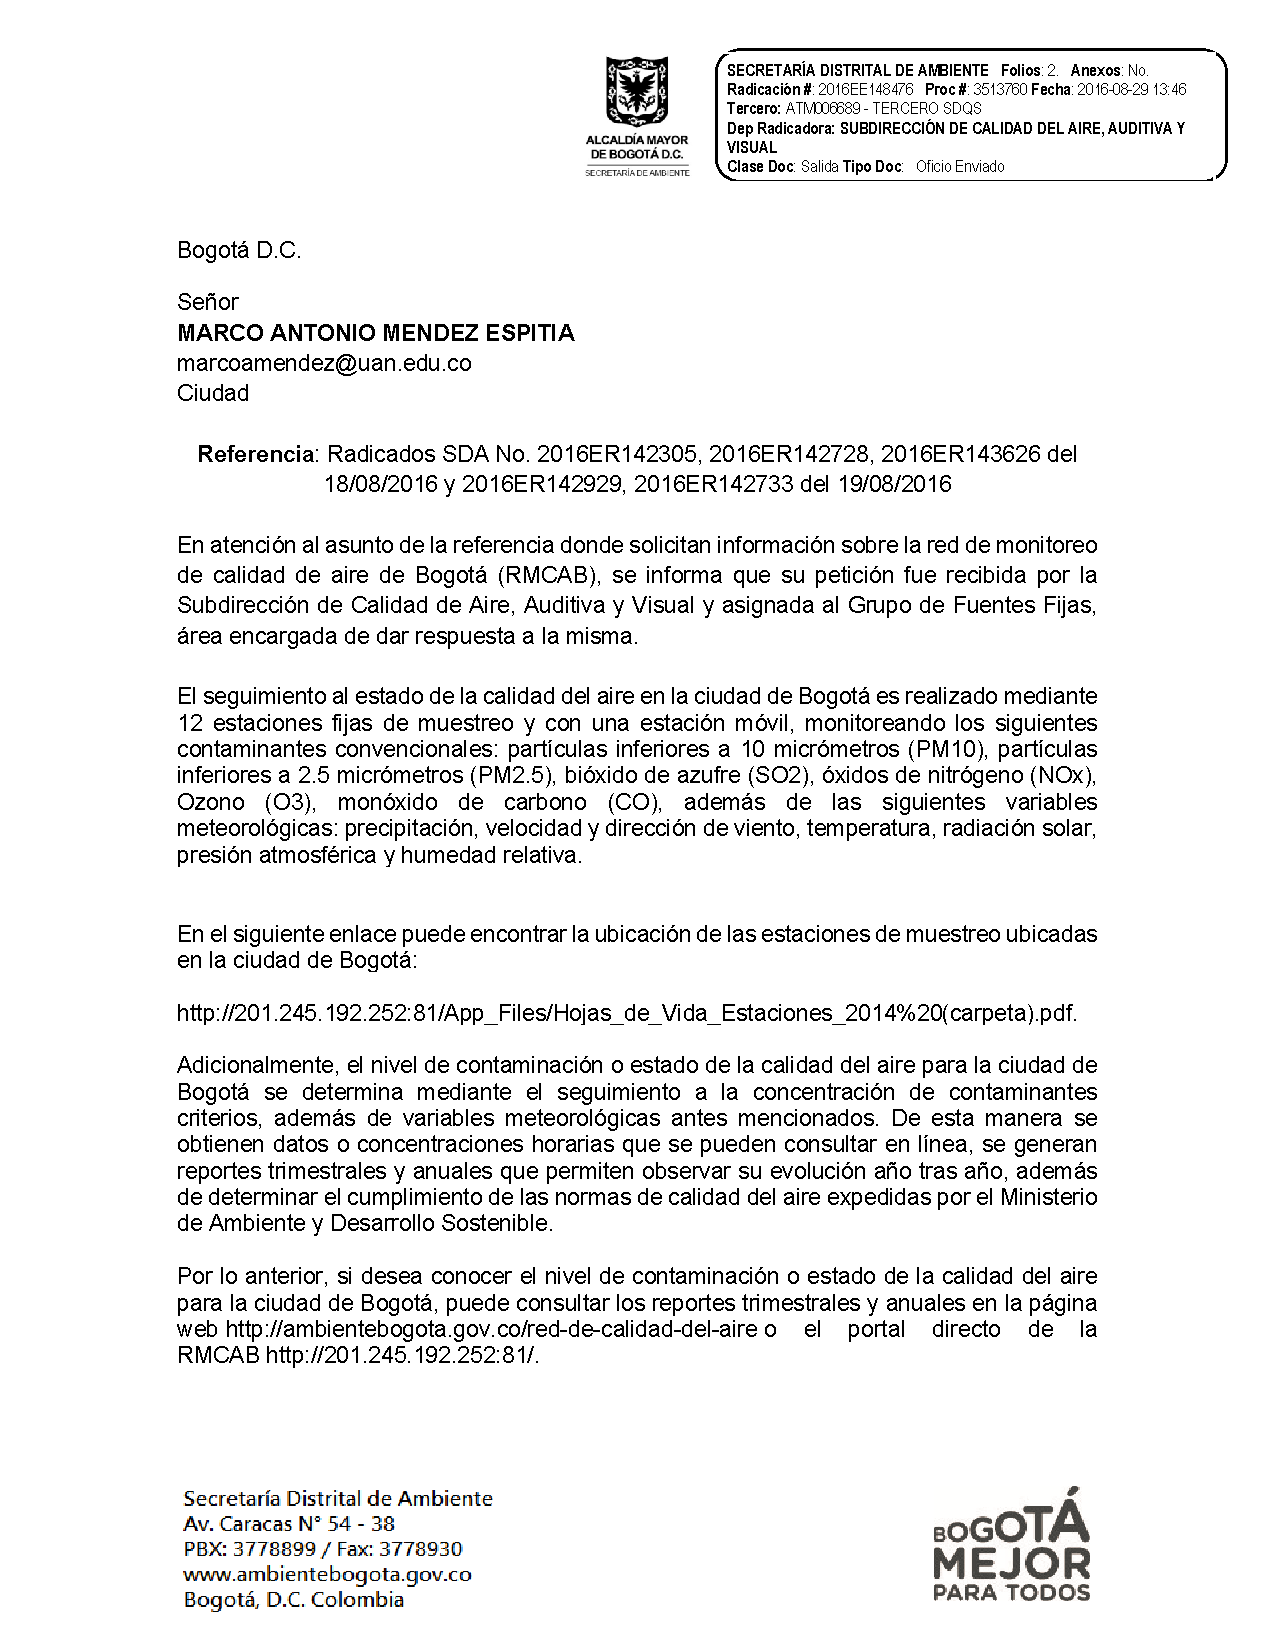
\includepdf[scale=0.8,pages=-]{Carta_SDA}
	\end{center}  
\textbf{ANEXO B.} 
    \begin{minted}[linenos,tabsize=2,breaklines]{python}
#Lineamientos para la anonimizacion de datos del sistema nacional de estudios y encuestas poblacionales para la salud Ministerio de Salud Y Proteccion Social Direccion de Epidemiologia y Demografia de Colombia
#Perturbacion - Anonimizacion de Datos RIPS
import xlrd as ex #Libreria para manejo de archivos Excel
import csv as c #Libreria para el manejo de archivos de extension csv
import numpy as np #Libreria para operaciones matematicas
import random as rd #Libreria para generar numeros aleatorios
import math
import operator

col = [[],[],[],[],[],[],[],[],[],[],[],[],[],[],[],[]] #Declaracion de una lista con 15 listas mas, donde se guardara las columnas de la lectura del archivo excel
micro = [[],[],[],[]]
columnas_alt = [1,2,12,13]
libro = ex.open_workbook("/Users/rlmendez/Desktop/sispro.rips.ira.2014DM.xls") #abrir el libro en la ruta determinada
sh = libro.sheet_by_index(0) #lectura a la primera hoja del libro
filas = sh.nrows #Cuenta el numero de filas ocupadas en la hoja seleccionada
columnas = sh.ncols #Cuenta el numero de columnas ocupadas en la hoja seleccionada
#Lectura del Archivo
f = 6 #Se inicializa en 6 para que inicie la lectura desde la fila 6 de la hoja de excel
x = 0 #Se inicializa en 0 indicando que se inicia la lectura desde la columna 0
while x<16: #Menor a 16 ya que son 15 iteraciones por el numero de columnas
	for f in range(filas-6): #No se lee los ultimos 6 registros
		col[x].append(sh.cell_value(f,x))  #lectura fila, columna y guardado en la lista
	x = x + 1
#Eliminacion de las primeras 5 registros
x = 0 
while x<16:
	col[x] = col[x][5:filas] #Se elimina los primeros 6 registros ya que son datos vacios o informacion que no es util
	x = x + 1
#PERTURBACION DE LAS COLUMNAS POR PERMUTACION
y = 0
for y in range(len(columnas_alt)):
	np.random.shuffle(col[columnas_alt[y]])
#Escritura de CSV POR PERMUTACION
with open('/Users/rlmendez/Desktop/sispro.rips.ira.2014DM_Permutacion.csv', 'wb') as csvsalida: #Crea un nuevo archivo en una ubicacion determinada
	wr = c.writer(csvsalida, delimiter=',') #delimita los datos a ingresar con coma ,
	for  lista in zip(*col): #realiza la transposicion de las listas en el archivo
		wr.writerow(lista) #Escribe los datos en el archivo csv
csvsalida.close() #cierra el archivo creado
#PERTURBACION DE LAS COLUMNAS POR MICROAGREGACION
datos = 360
k = 3
k1 = datos/k
for r in columnas_alt:
	diccionario_aux = {}
	posiciones = []
	valores = []
	prom = []
	x = 0
	while x<len(col[r]):
		diccionario_aux[x]=col[r][x]
		x+=1
	for clave, valor in sorted(diccionario_aux.items(), key=operator.itemgetter(1)):
		posiciones.append(clave)
		valores.append(valor)	
	inicio = 0
	final = k-1
	for t in range(0,k1):
		aux = np.average(valores[inicio:final])
		prom.append(aux)
		inicio +=k
		final +=k
	pos = 0
	for b in range(len(prom)):
		valores[pos] = prom[b]
		valores[pos+1] = prom[b]
		valores[pos+2] = prom[b]
		pos += k
	for x in range(len(posiciones)):
		for clave, valor in diccionario_aux.iteritems():
			if posiciones[x]==clave:
				diccionario_aux[posiciones[x]] = valores[x]
	col[r] = diccionario_aux.values()
#Escritura de CSV POR PERMUTACION
with open('/Users/rlmendez/Desktop/sispro.rips.ira.2014DM_Microagregacion.csv', 'wb') as csvsalida: #Crea un nuevo archivo en una ubicacion determinada
	wr = c.writer(csvsalida, delimiter=',') #delimita los datos a ingresar con coma ,
	for  lista in zip(*col): #realiza la transposicion de las listas en el archivo
		wr.writerow(lista) #Escribe los datos en el archivo csv
csvsalida.close() #cierra el archivo creado
\end{minted}
\end{document}

-